\documentclass[12pt,a4paper]{article}
\usepackage[utf8]{inputenc}\usepackage[T1]{fontenc}\usepackage[brazil]{babel}\usepackage{lmodern}
\usepackage{geometry}\geometry{margin=2.3cm}\usepackage{graphicx}\graphicspath{{figuras/}}
\usepackage{booktabs,tabularx,array,amsmath,amssymb,siunitx,xcolor,float}\sisetup{output-decimal-marker={,}}
\usepackage[section]{placeins}\usepackage{enumitem,microtype,caption,subcaption,listings,hyperref,fancyhdr}
\hypersetup{colorlinks=true,linkcolor=blue!55!black,urlcolor=blue!55!black,citecolor=blue!55!black}
\lstdefinestyle{sindyeq}{basicstyle=\ttfamily\scriptsize,breaklines=true,columns=fullflexible,frame=single,numbers=left,numberstyle=\tiny\color{gray},xleftmargin=1.5em,framexleftmargin=1.2em,showstringspaces=false}
\pagestyle{fancy}\fancyhf{}\lhead{Cavidade URANS e modelos reduzidos}\rhead{Relatório técnico}\cfoot{\thepage}
\setlength{\parindent}{1.2em}\setlength{\parskip}{.35em}\newcommand{\code}[1]{\texttt{#1}}
\title{\textbf{Relatório técnico do caso cavity 10 000}\\[.4em]OpenFOAM, POD, SAE e identificação dinâmica SINDy}
\author{Análise dos códigos e artefatos armazenados no caso}\date{\today}
\begin{document}\maketitle
\begin{abstract}
Este relatório analisa uma cavidade com tampa móvel calculada pelo OpenFOAM 13 com escoamento compressível, gás perfeito e URANS $k$--$\omega$ SST, além das reduções POD e SAE e dos modelos POD--SINDy, SAE--SINDy e SAE--POD--SINDy. A POD legada salva 5646 snapshots, mas foi configurada com campos de dam-break: $\alpha_{water}$ e $p_{rgh}$ não existem e foram preenchidos com zeros. Após a auditoria, uma POD corrigida com $U_x,U_y,p,T,k$ foi calculada em 5645 snapshots válidos: 50 modos preservam 99,988\% da energia e apresentam erro global de 1,083\%. O SAE usa corretamente $U,p,T,k$, alcançando $R^2=0,809$ no treino e 0,825 na validação. POD--SINDy e SAE--SINDy falham na integração livre principal. A POD estabilizadora conserva 96,68\% da energia latente e permite integração livre, mas o erro é 0,644 e $R^2=0,586$. Um comparador adicional contra OpenFOAM bruto está temporalmente incorreto e não pode ser usado para validação.
\end{abstract}
\tableofcontents\listoffigures\listoftables\clearpage

\section{Escopo, fontes e rastreabilidade}
O caso está em
\begin{quote}\small\path{/home/mlep-pc-ubuntu/OpenFOAM/mlep-pc-ubuntu-13/run/cavity 10 000}.\end{quote}
Foram examinados os dicionários OpenFOAM, 5646 diretórios temporais presentes, notebooks e artefatos NPZ, Keras e JSON. Os modelos não foram reexecutados; os números são os efetivamente armazenados.

Há duas ressalvas centrais. Primeiro, a POD pede \code{U}, \code{alpha.water}, \code{p\_rgh} e \code{k}; neste caso existem $U$, $p$, $T$, $k$, $\omega$, $\rho$ e campos auxiliares, mas não $\alpha_{water}$ nem $p_{rgh}$. O leitor insere zeros silenciosamente. Assim, dos cinco canais POD, apenas $U_x,U_y,k$ são físicos. Segundo, o comparador OpenFOAM bruto--SINDy supõe que o conjunto OpenFOAM termina em $1\,\si{s}$, enquanto os latentes terminam em $4,9965\,\si{s}$. Depois de 1 s ele compara estados com diferenças temporais de até 3,9965 s.

\section{Modelo OpenFOAM}
\subsection{Geometria, condições e propriedades}
A malha é um quadrado $0,1\times0,1\,\si{m^2}$ com espessura $0,01\,\si{m}$, discretizado em $40\times40\times1=1600$ células uniformes. As faces frontal e traseira são \code{empty}; portanto, o problema é bidimensional. A tampa \code{movingWall} tem $U=(1,0,0)\,\si{m.s^{-1}}$ e as outras paredes são estacionárias. A pressão possui gradiente normal nulo nas paredes.

O solver genérico \code{fluid} resolve gás perfeito com $M=28,9\,\si{kg.kmol^{-1}}$, $C_p=1007\,\si{J.kg^{-1}.K^{-1}}$, viscosidade dinâmica $\mu=1,84\times10^{-5}\,\si{Pa.s}$ e $Pr=0,7$. O transporte de momento é RAS com $k$--$\omega$ SST e turbulência ativada. O nome ``10 000'' sugere Reynolds nominal, mas o relatório não infere esse valor apenas do nome; ele deve ser confirmado com densidade/temperatura de referência e definição adotada.

\subsection{Discretização}
\begin{table}[H]\centering\caption{Configuração numérica do OpenFOAM.}\label{tab:foam}
\begin{tabularx}{\textwidth}{>{\bfseries}l X}\toprule Item&Configuração\\\midrule
Intervalo nominal&$0\le t\le5\,\si{s}$, $\Delta t=5\times10^{-4}\,\si{s}$, saída a cada passo\\
Dados presentes&5646 tempos entre 0,001 e 5 s; sequência irregular/incompleta\\
Tempo&Euler de primeira ordem\\
Gradientes&Gauss linear\\
Momento&Gauss \code{limitedLinearV 1}\\
$k,\omega$&Gauss \code{limitedLinear 1}\\
Laplaciano e $\mathrm{snGrad}$&linear orthogonal / orthogonal\\
Passo adaptativo&desligado; \code{maxCo}=0,3 não reduz $\Delta t$\\
Formato de saída&binário, precisão declarada 10\\\bottomrule\end{tabularx}\end{table}

\begin{table}[H]\centering\caption{Solvers e acoplamento.}\label{tab:solver}
\begin{tabularx}{\textwidth}{>{\bfseries}l X}\toprule Variável&Configuração\\\midrule
$p$&PCG/DIC, tolerância $10^{-6}$, \code{relTol}=0,01; final com \code{relTol}=0\\
$U,h,k,\omega$&\code{smoothSolver}/\code{symGaussSeidel}, tolerância $10^{-5}$, \code{relTol}=0,1\\
PIMPLE&preditor de momento; 1 corretor externo, 2 internos, nenhum não ortogonal\\\bottomrule\end{tabularx}\end{table}

São positivos a malha ortogonal, formulação quase 2D clara e gravação densa. São limitações o Euler de primeira ordem, ausência de adaptação pelo Courant, dados temporais faltantes e ausência de estudo de malha/passo ou comparação com perfis clássicos da cavidade.

\section{POD}
A decomposição da matriz centralizada e normalizada por snapshot é
\begin{equation}X-\bar X=U\Sigma V^T,\qquad X_r=U_r\Sigma_rV_r^T.\end{equation}
A matriz tem $8000\times5646$: 1600 células e cinco canais declarados. Como dois canais são zeros, a excelente compressibilidade deve ser interpretada como referente sobretudo a $U_x,U_y,k$.

\begin{table}[H]\centering\caption{Energia e erro POD.}\label{tab:pod}
\begin{tabular}{rcc}\toprule Modos&Energia acumulada&Erro global\\\midrule
1&0,67979&0,56587\\2&0,82148&0,42252\\4&0,93675&0,25149\\8&0,98650&0,11619\\16&0,99872&0,03576\\32&0,99994&0,00775\\50&0,99999&0,00323\\\bottomrule\end{tabular}\end{table}

\begin{figure}[H]\centering
\begin{subfigure}{.49\textwidth}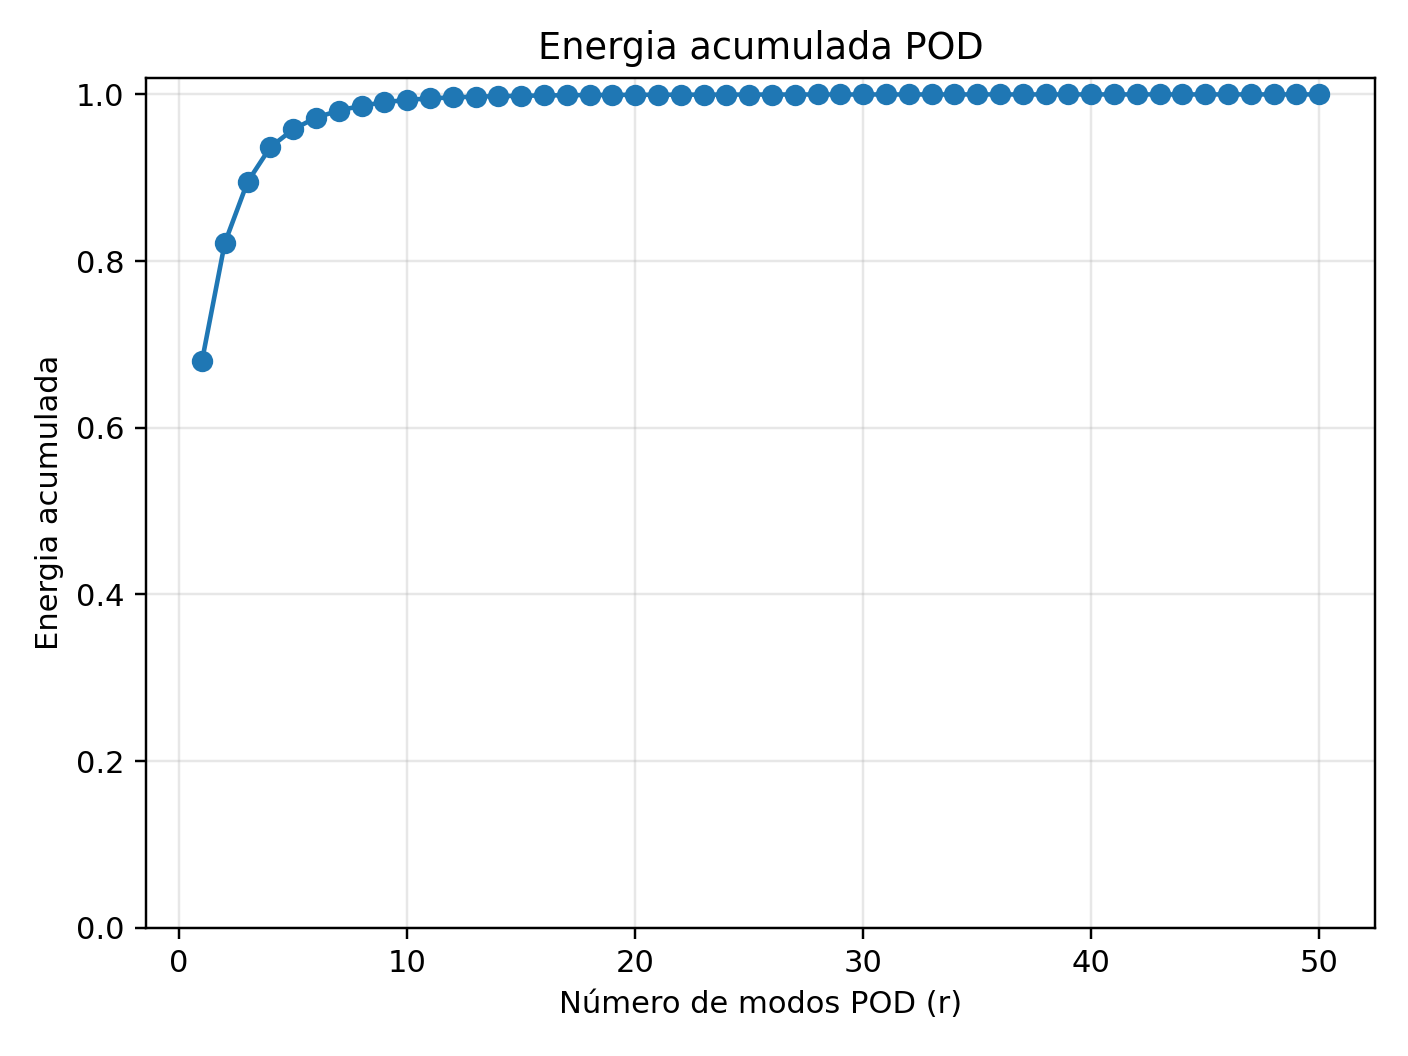
\includegraphics[width=\linewidth]{pod_energia.png}\caption{Energia.}\end{subfigure}
\begin{subfigure}{.49\textwidth}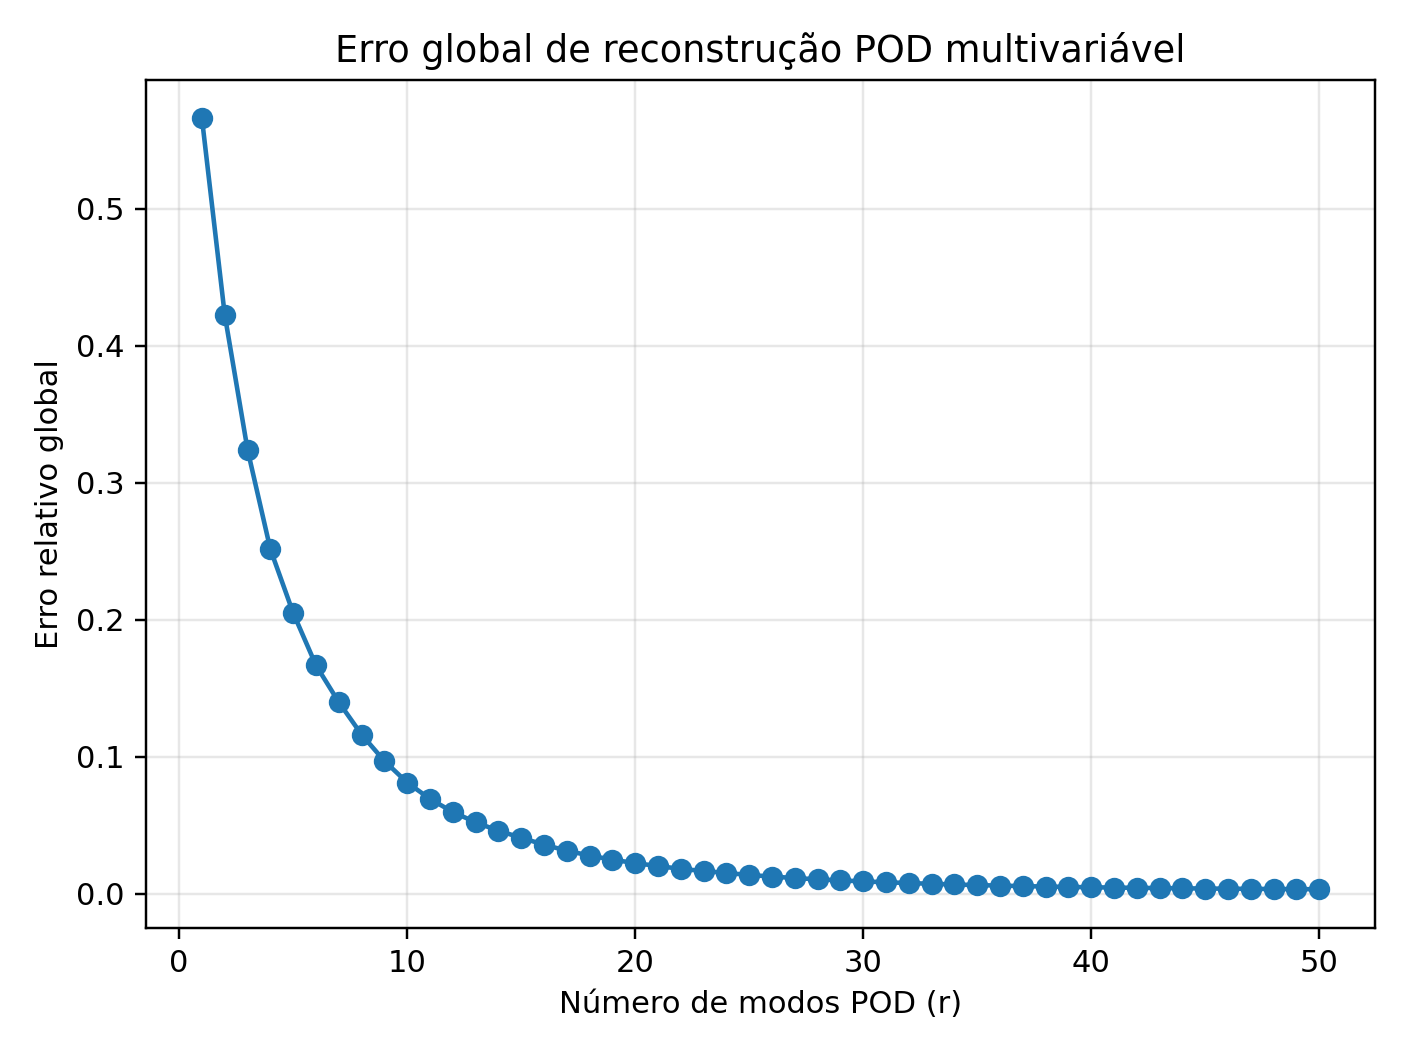
\includegraphics[width=\linewidth]{pod_erro.png}\caption{Erro global.}\end{subfigure}
\caption{Convergência POD.}\end{figure}
\begin{figure}[H]\centering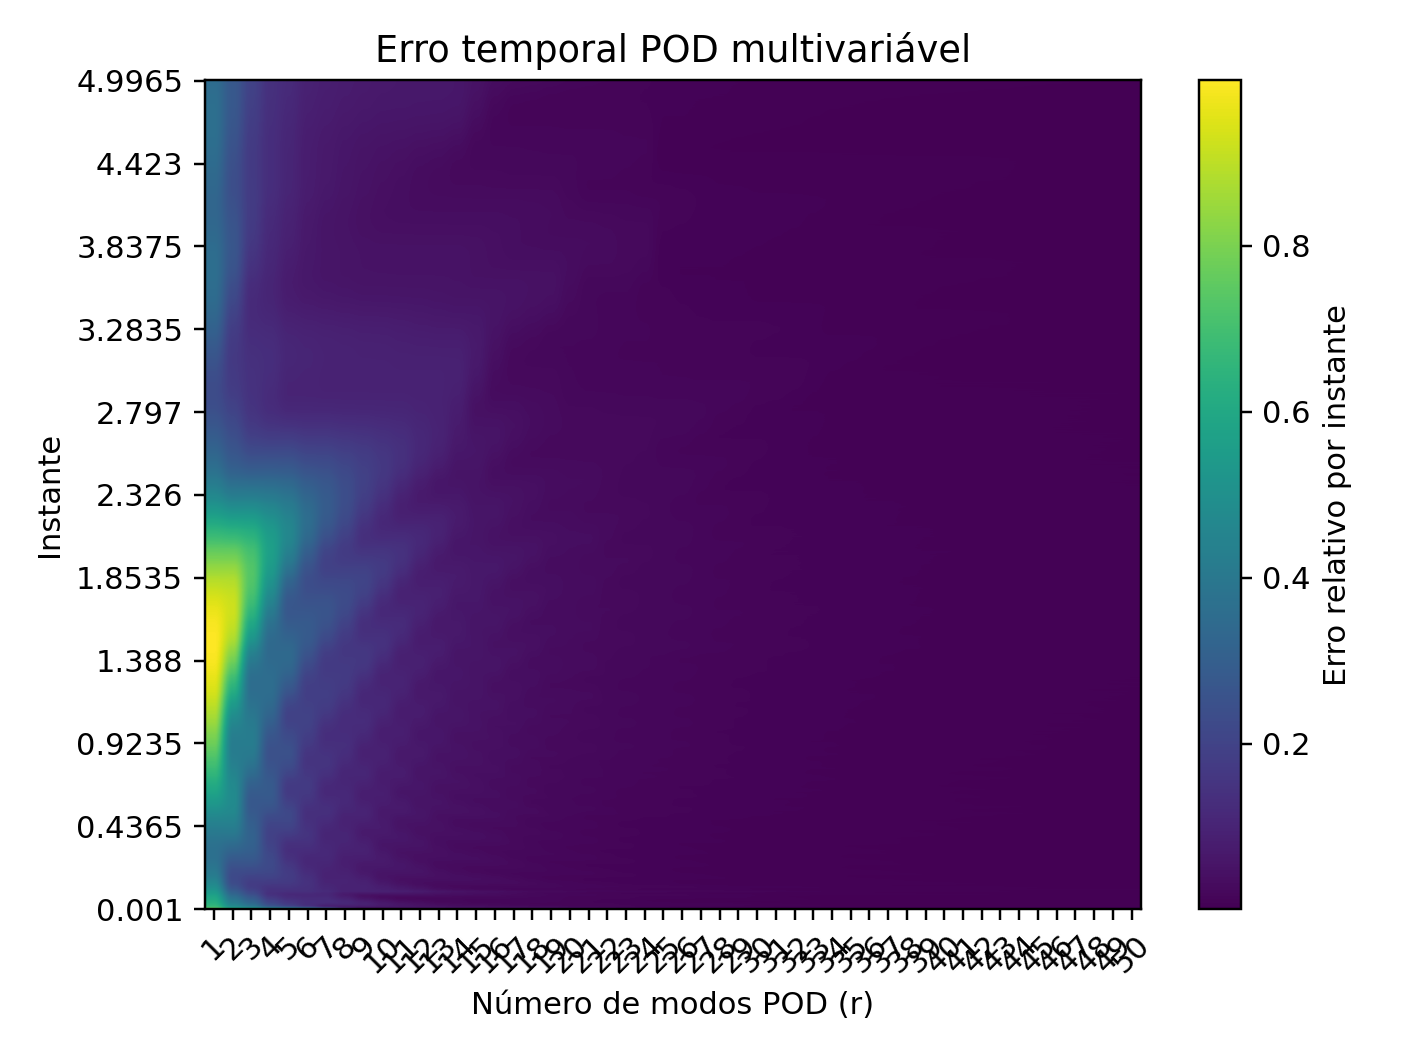
\includegraphics[width=.88\textwidth]{pod_mapa.png}\caption{Erro temporal POD. Com 50 modos, o máximo é 0,00626.}\end{figure}
\begin{figure}[H]\centering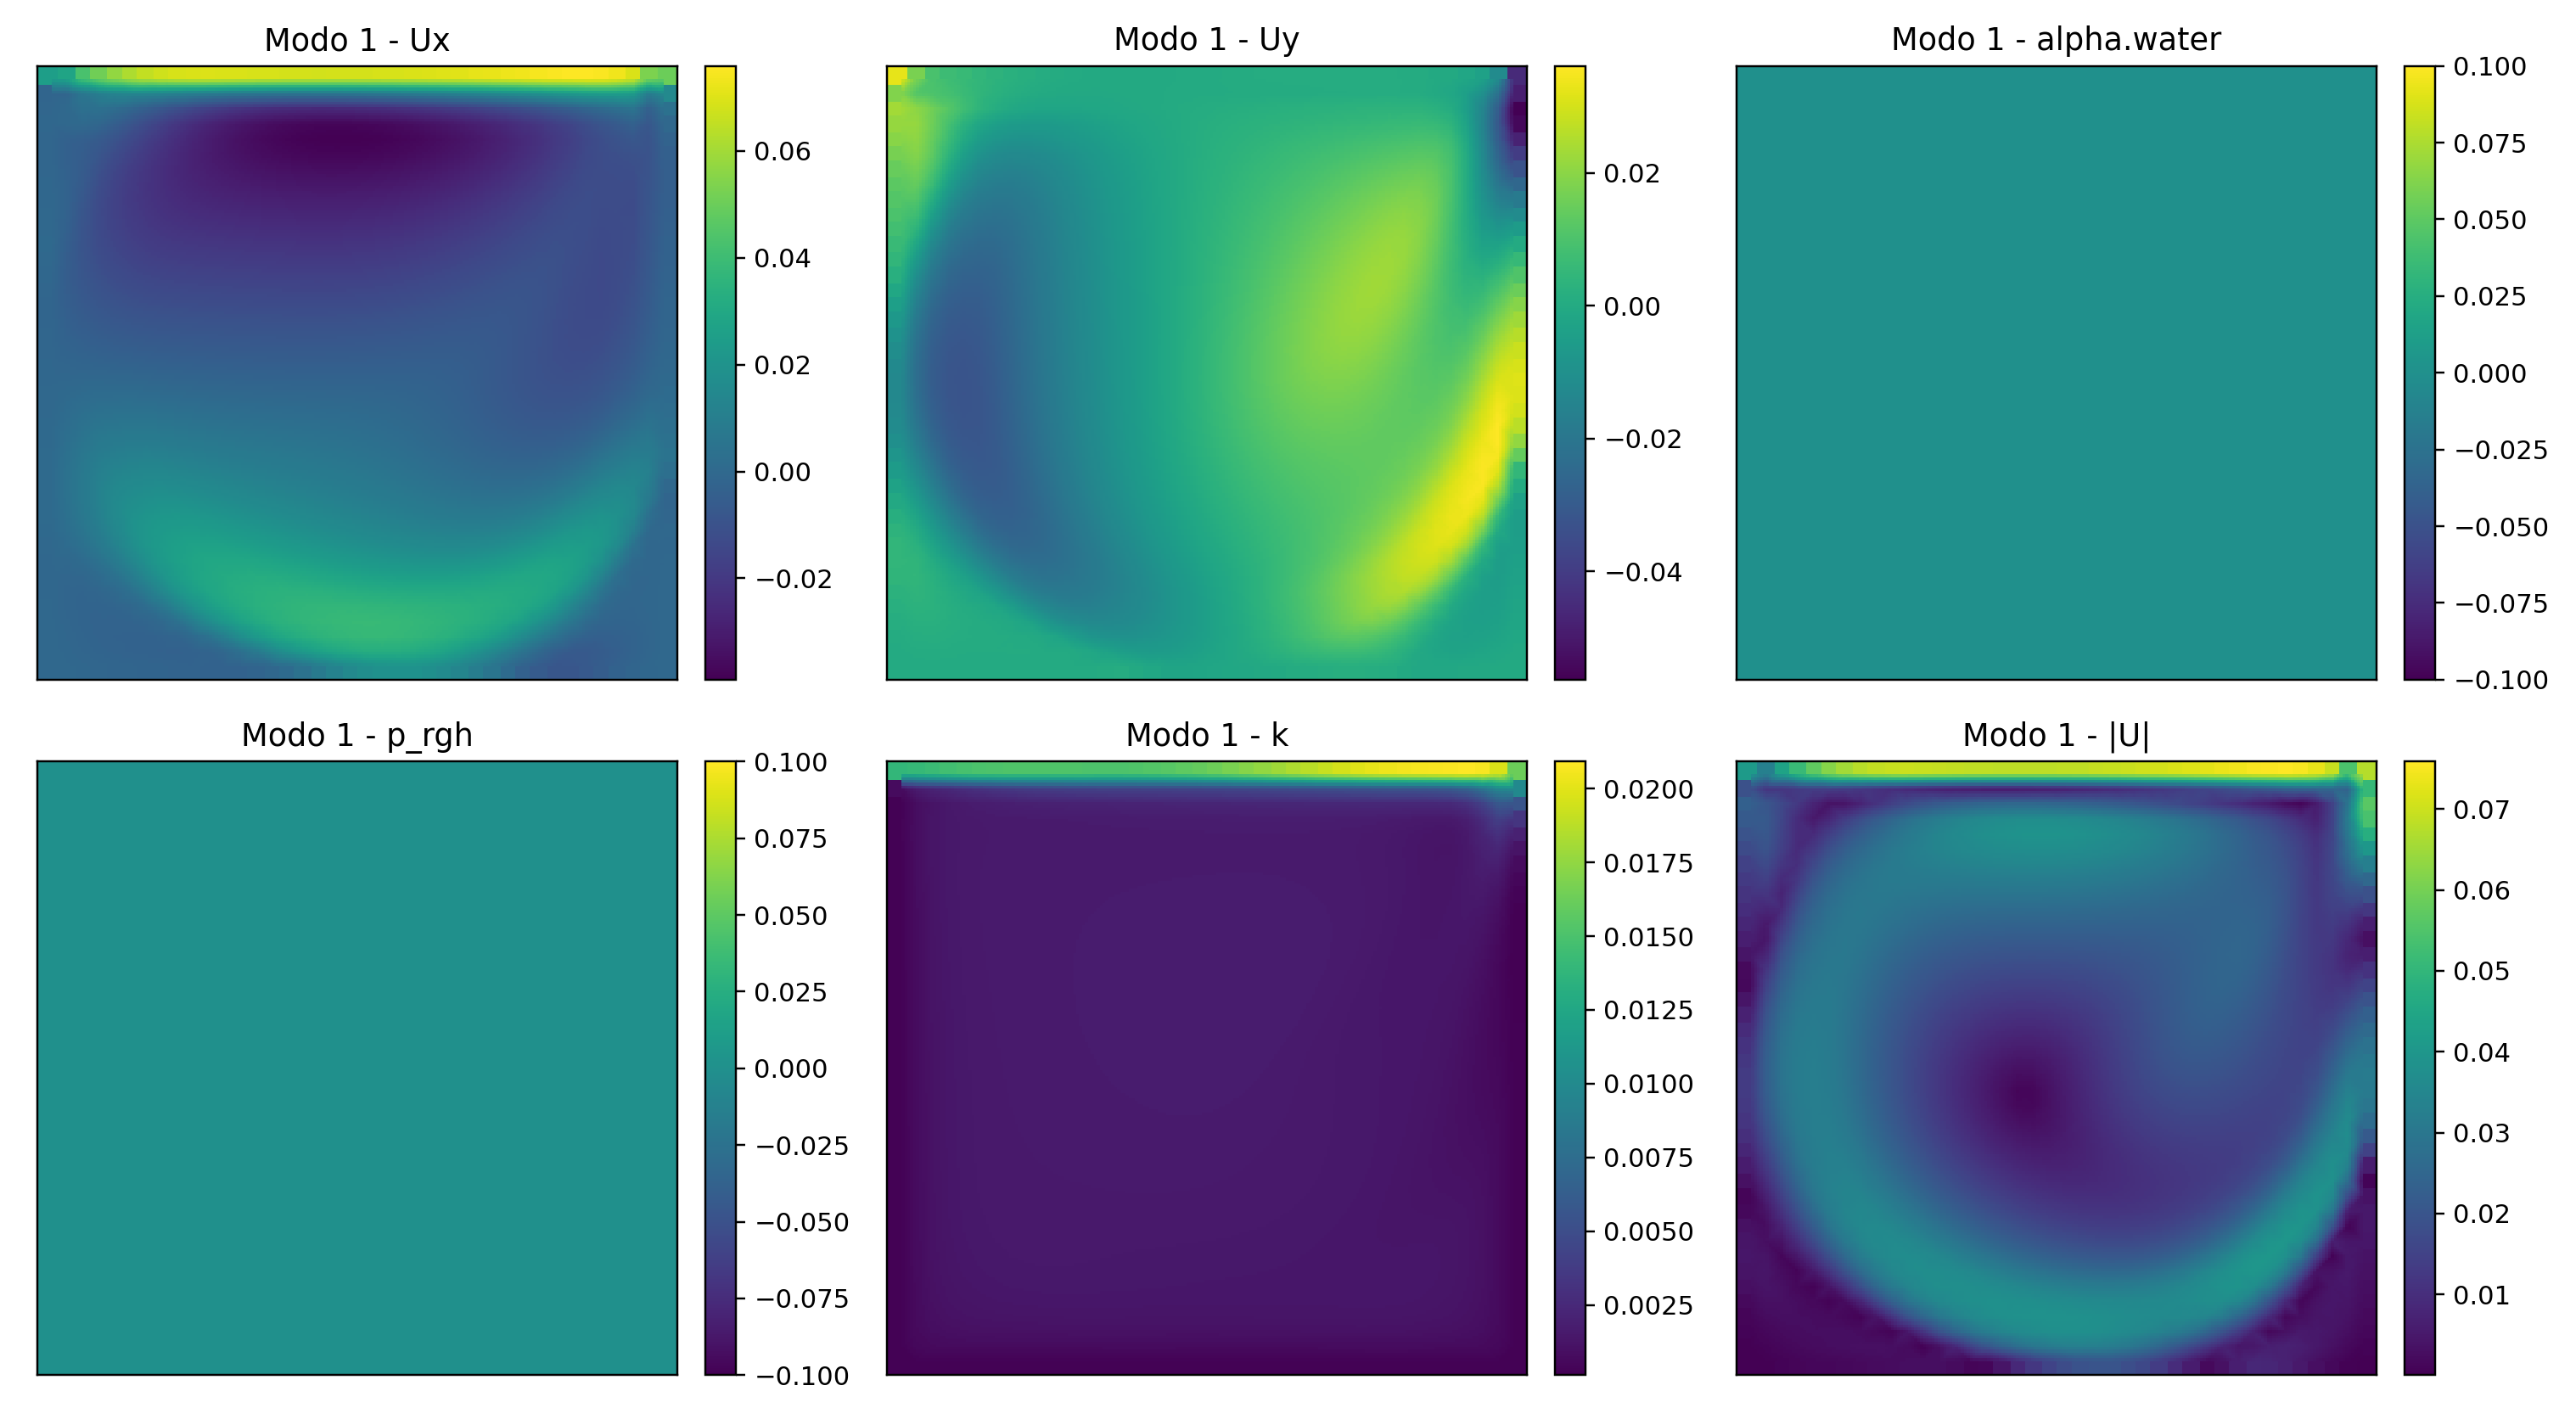
\includegraphics[width=.95\textwidth]{pod_modo1.png}\caption{Primeiro modo POD. Os canais rotulados $\alpha_{water}$ e $p_{rgh}$ são artificiais e nulos.}\end{figure}
\begin{figure}[H]\centering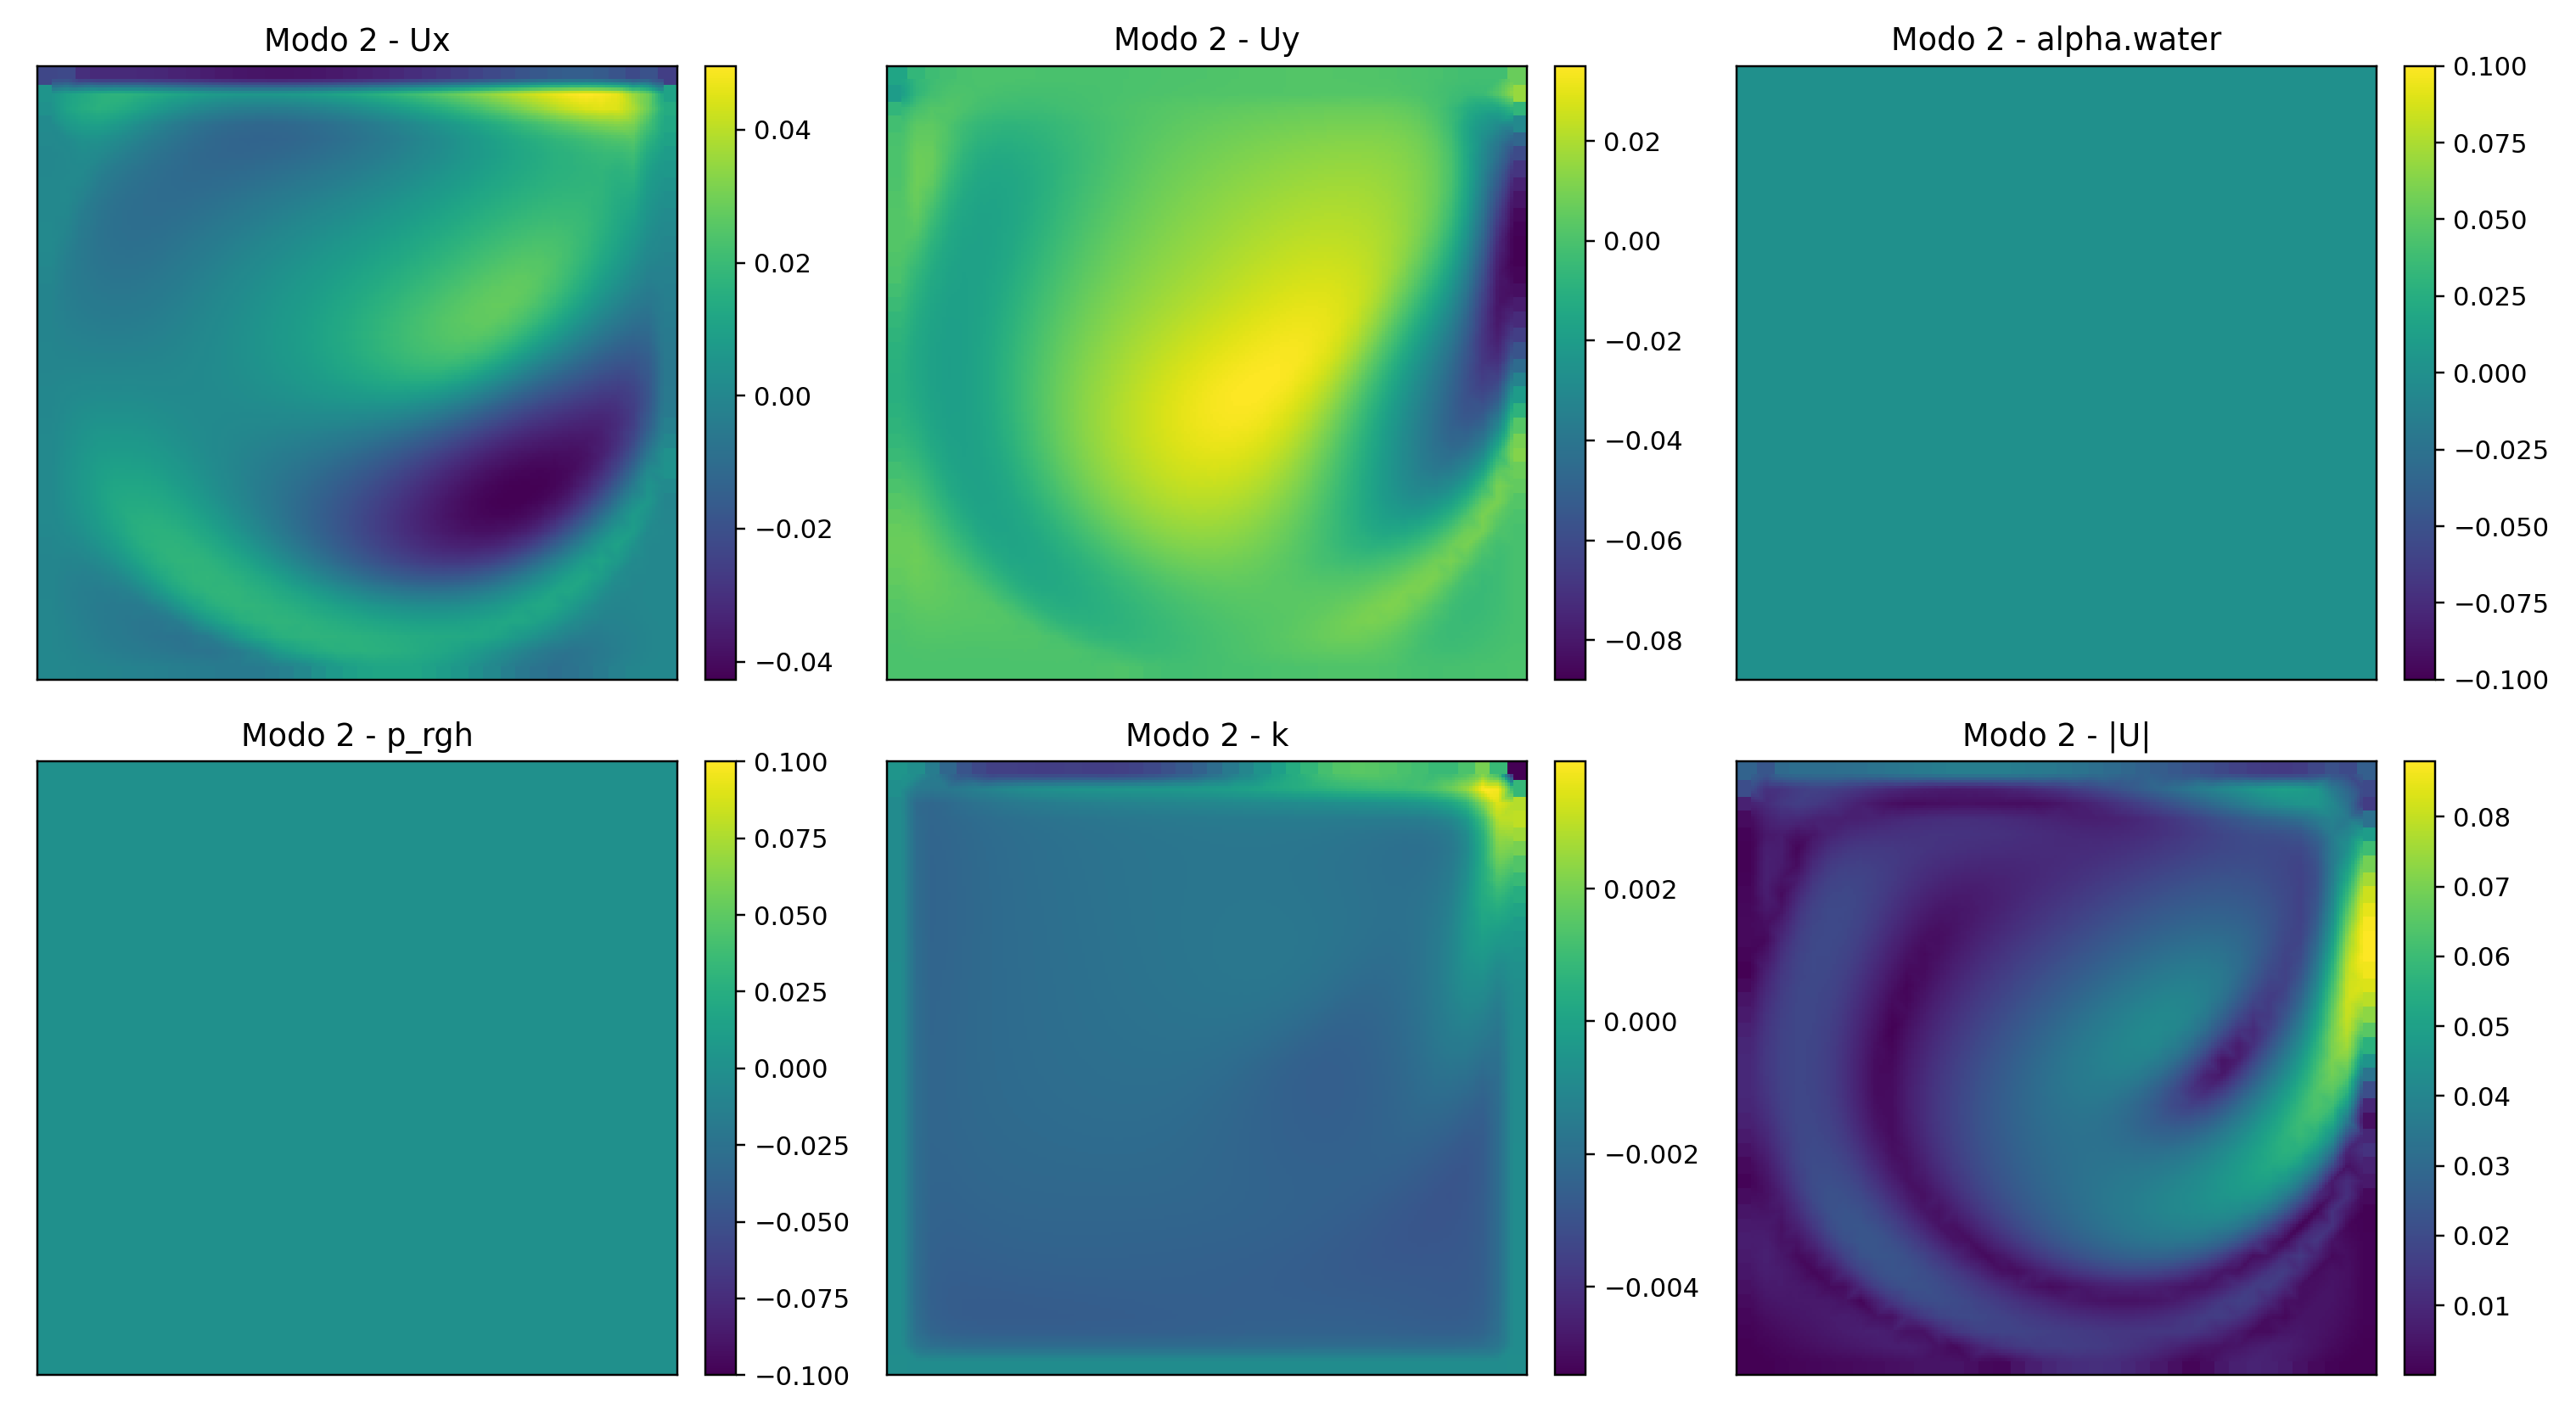
\includegraphics[width=.95\textwidth]{pod_modo2.png}\caption{Segundo modo POD.}\end{figure}
\begin{figure}[H]\centering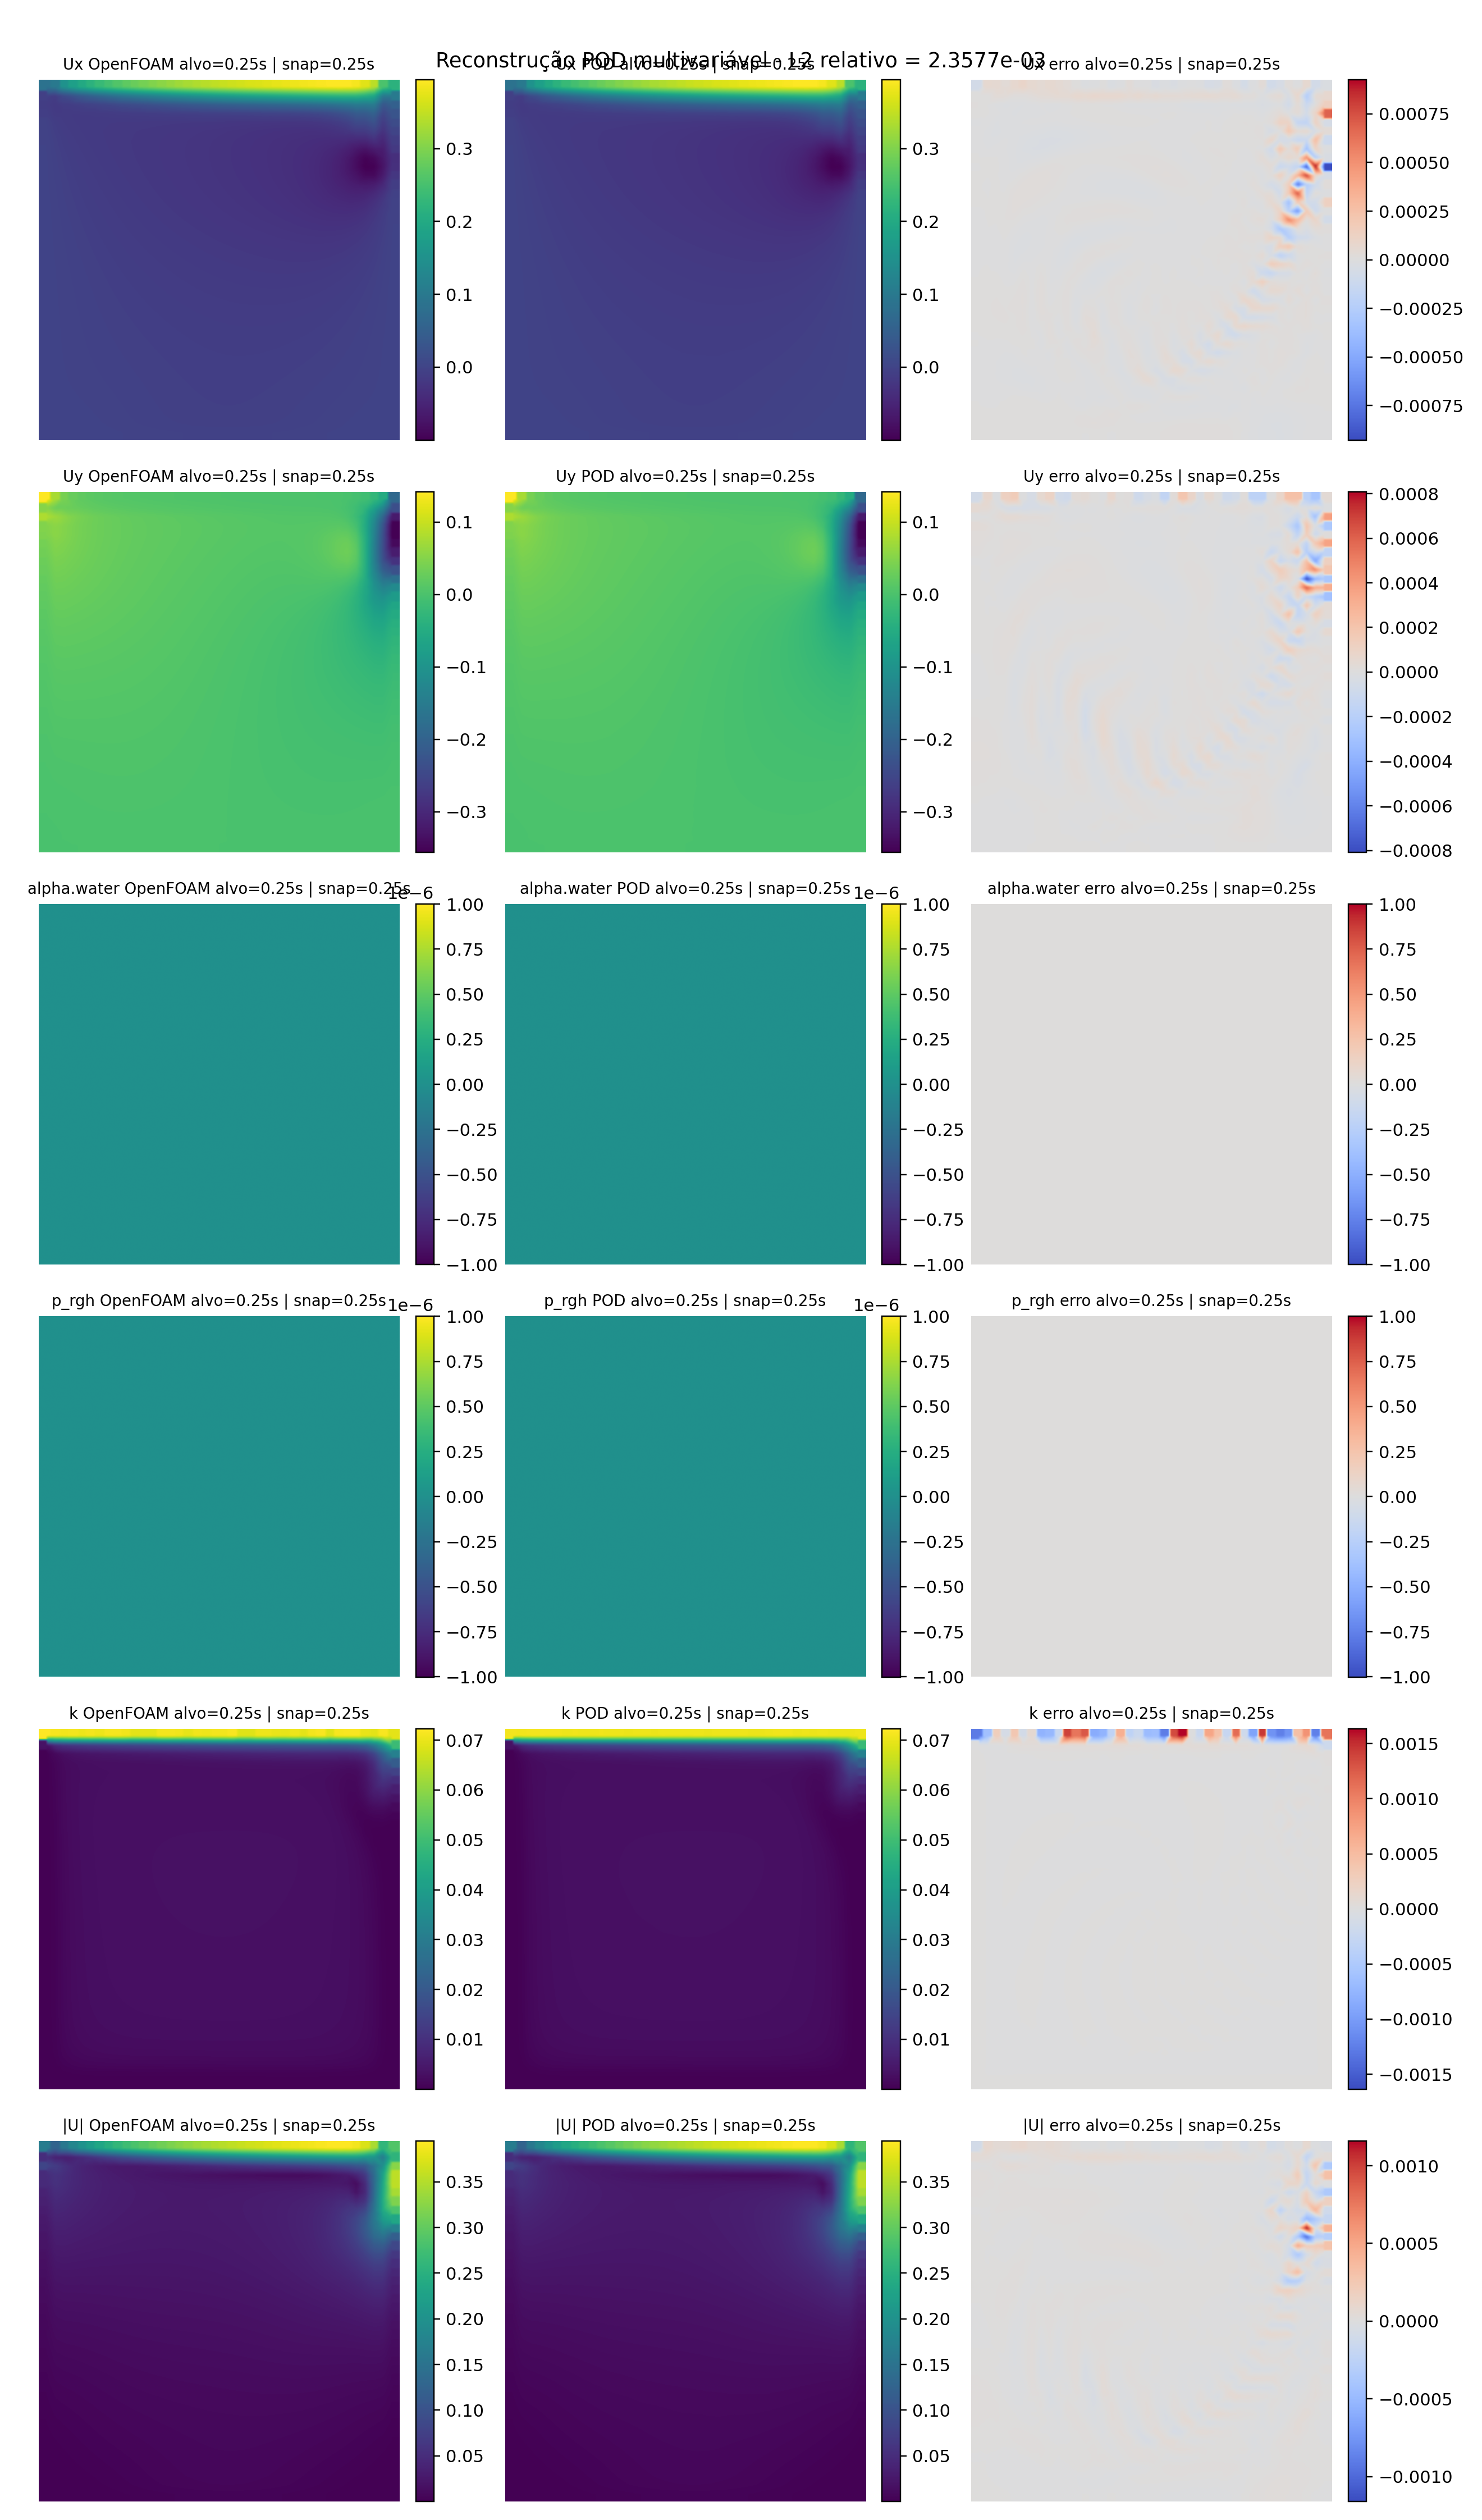
\includegraphics[height=.79\textheight,keepaspectratio]{pod_t025.png}\caption{Reconstrução POD em $t\approx0,25\,\si{s}$, incluindo os canais inválidos.}\end{figure}
\begin{figure}[H]\centering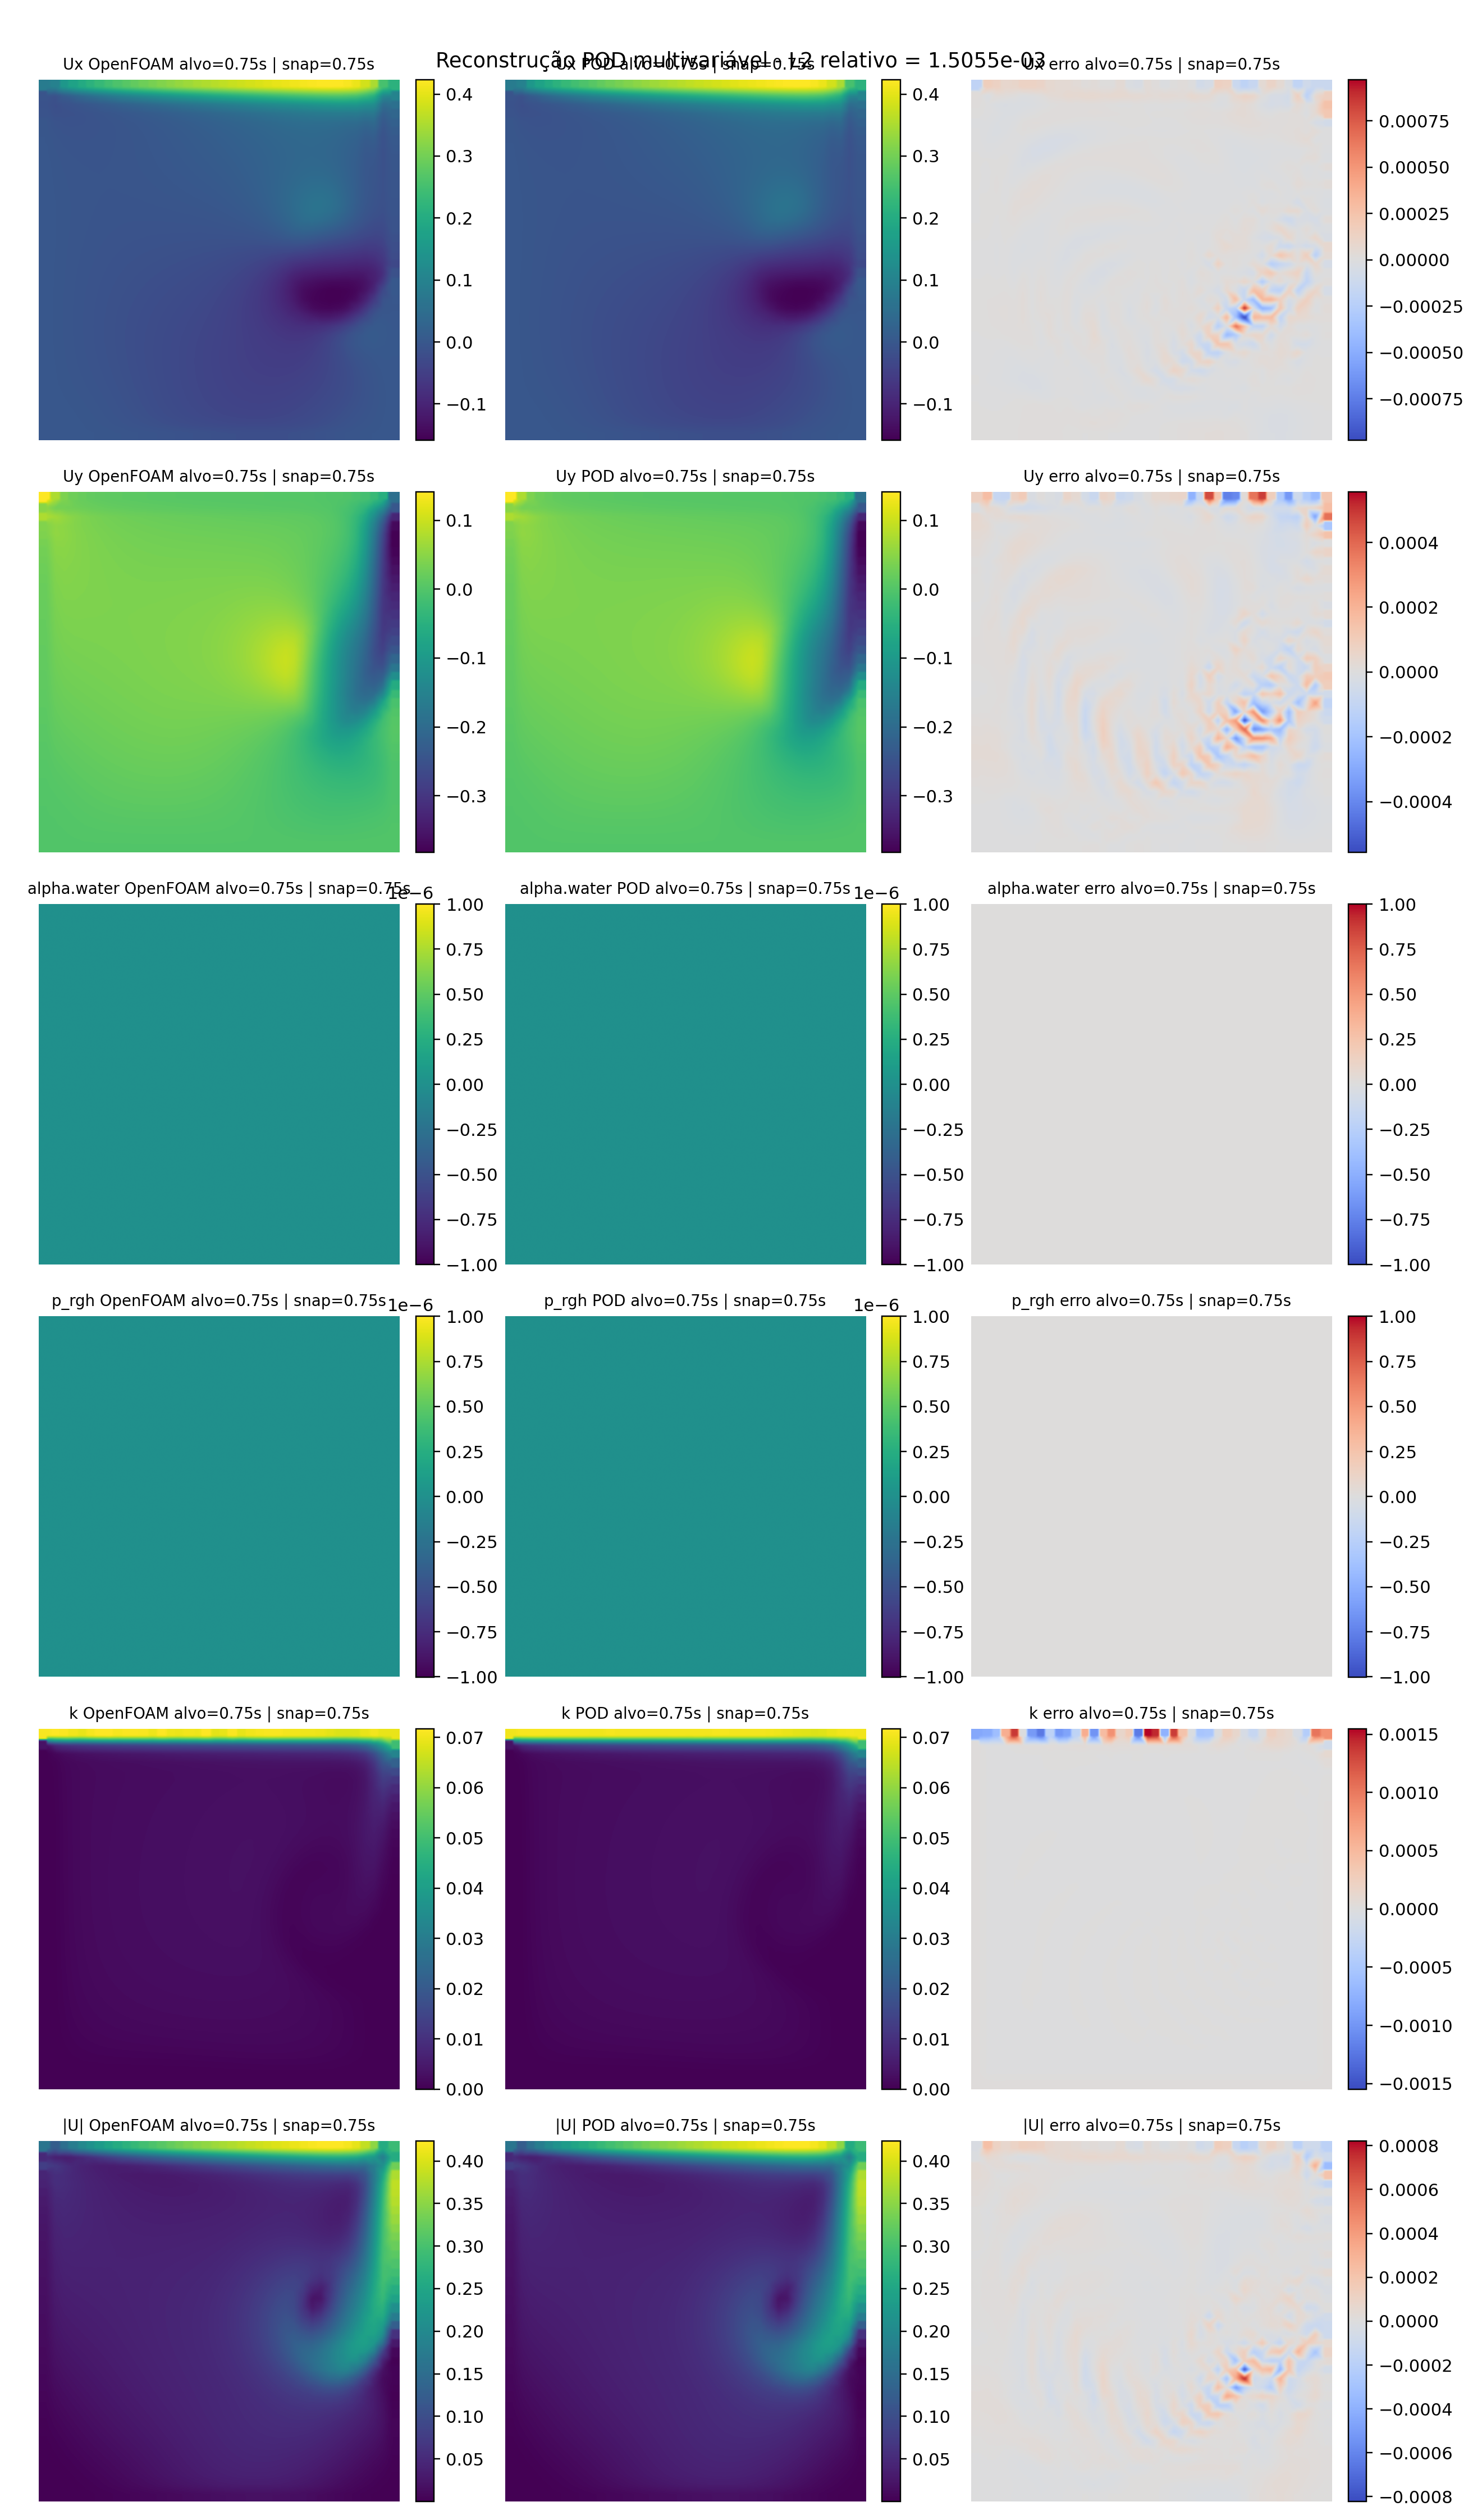
\includegraphics[height=.79\textheight,keepaspectratio]{pod_t075.png}\caption{Reconstrução POD em $t\approx0,75\,\si{s}$.}\end{figure}

\subsection{POD corrigida após a auditoria}
A nova execução usa $U_x,U_y,p,T,k$, não normaliza cada snapshot e rejeita explicitamente dados incompletos. Dos 5646 diretórios, o instante $t=3,2185\,\si{s}$ foi excluído porque não contém $p$ nem $T$, restando 5645 snapshots. Uma SVD aleatorizada com 50 modos, sete iterações e semente 7 reduz o custo de memória sem construir matrizes quadradas desnecessárias.

\begin{table}[H]\centering\caption{POD corrigida com campos físicos da cavidade.}\label{tab:podcorr}
\begin{tabular}{rcc}\toprule Modos&Energia acumulada&Erro global\\\midrule
8&0,99303&0,08349\\16&0,99886&0,03381\\50&0,99988&0,01083\\\bottomrule\end{tabular}\end{table}
\begin{figure}[H]\centering
\begin{subfigure}{.49\textwidth}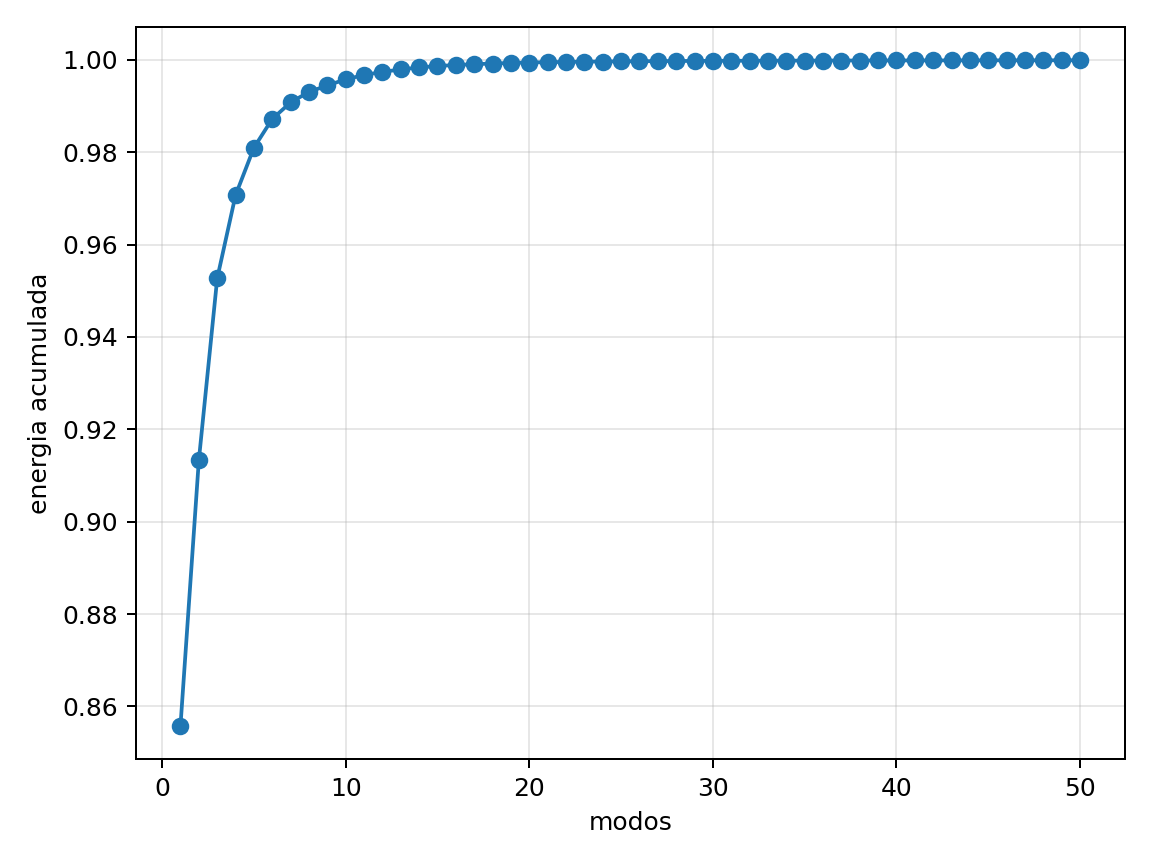
\includegraphics[width=\linewidth]{pod_corr_energia.png}\caption{Energia corrigida.}\end{subfigure}
\begin{subfigure}{.49\textwidth}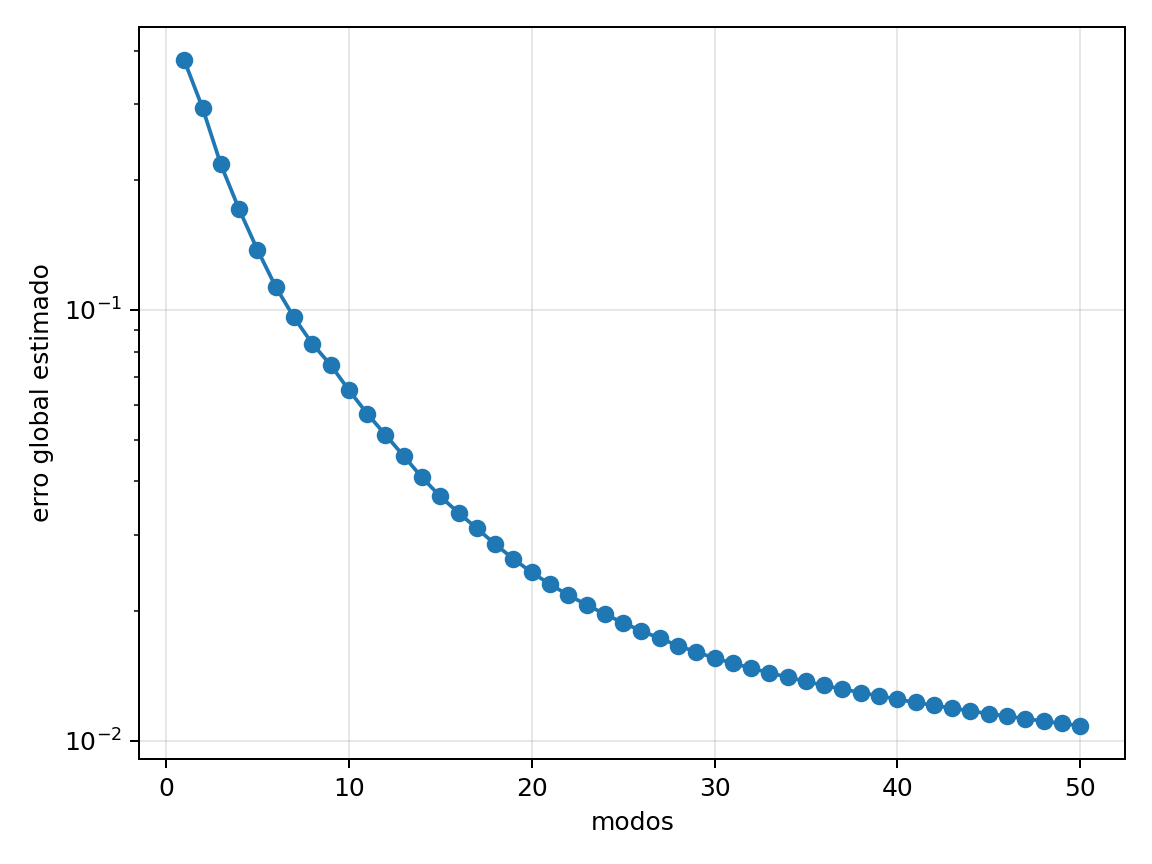
\includegraphics[width=\linewidth]{pod_corr_erro.png}\caption{Erro corrigido.}\end{subfigure}
\caption{Convergência da POD de $U_x,U_y,p,T,k$ em unidades físicas.}\end{figure}
\begin{figure}[H]\centering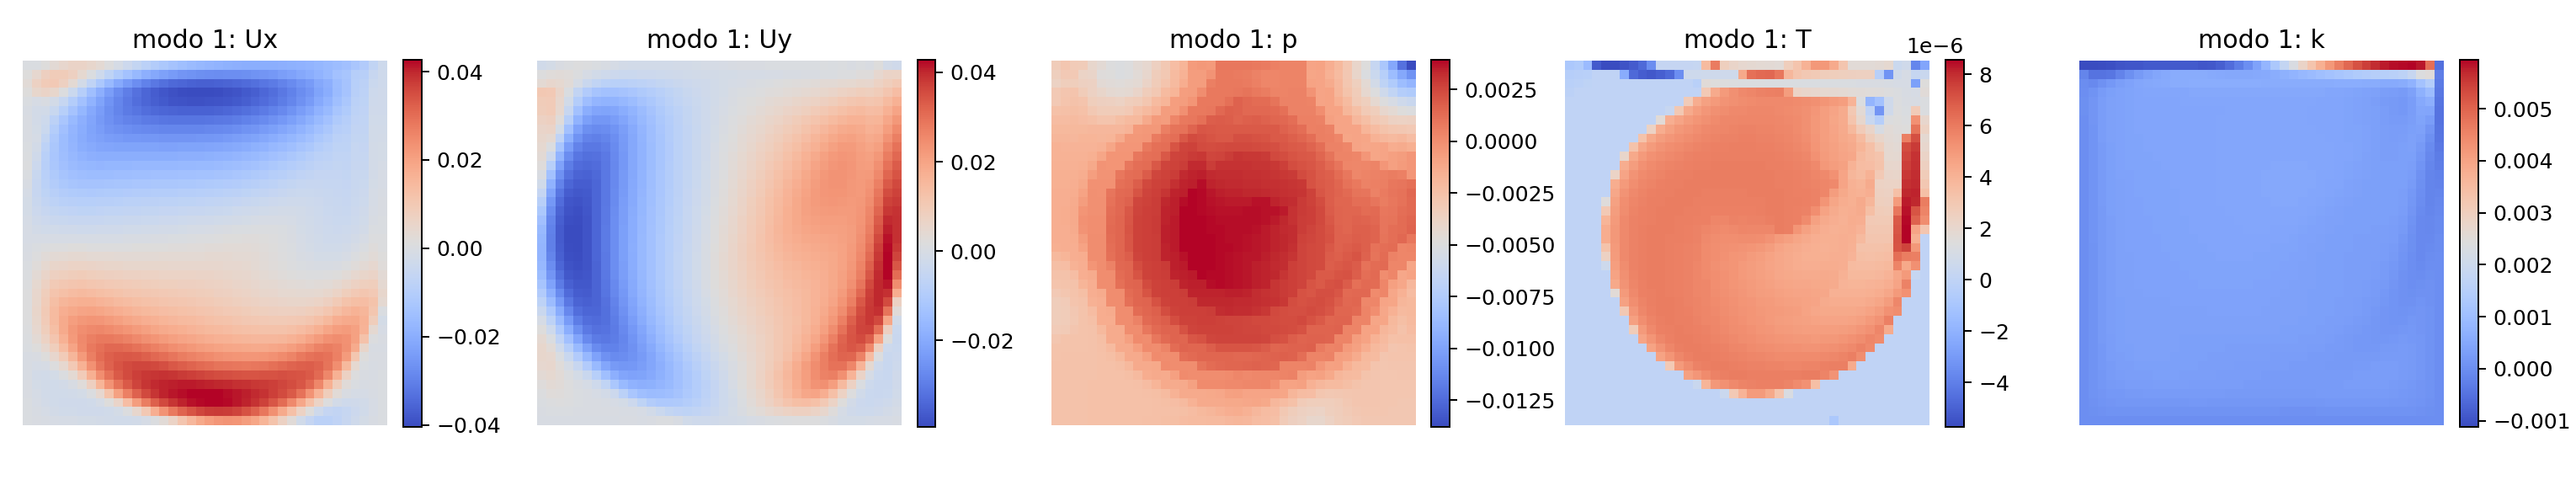
\includegraphics[width=.95\textwidth]{pod_corr_modo1.png}\caption{Primeiro modo POD corrigido.}\end{figure}
\begin{figure}[H]\centering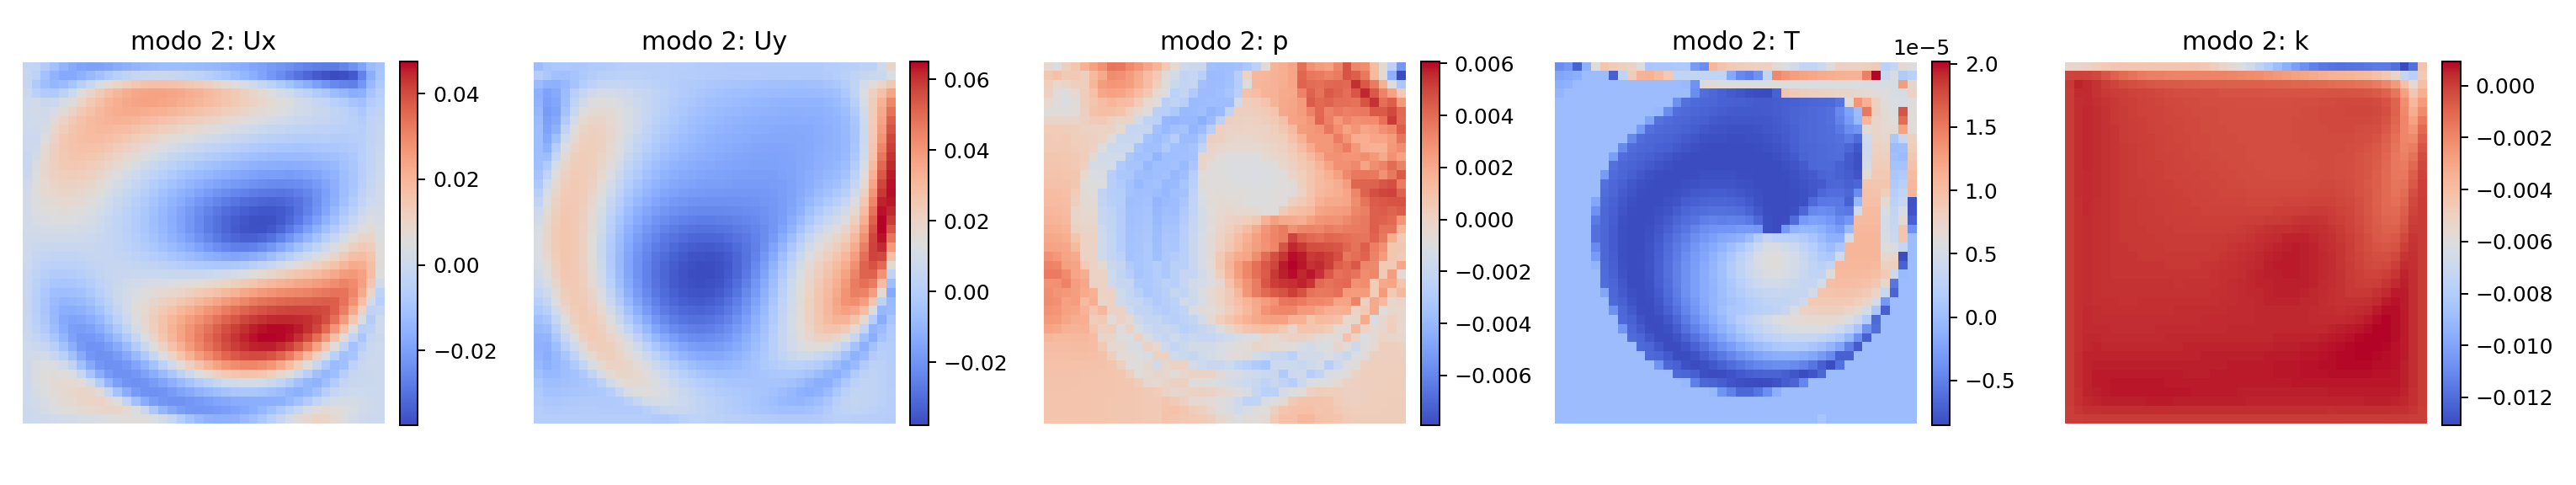
\includegraphics[width=.95\textwidth]{pod_corr_modo2.png}\caption{Segundo modo POD corrigido.}\end{figure}

\section{SAE}
O SAE interpola $U_x,U_y,p,T,k$ numa grade $48\times48$, totalizando 11520 entradas. O encoder 128--64--32 produz oito latentes; o decoder é simétrico. Usa Adam com taxa inicial $5\times10^{-5}$, Huber, Batch Normalization, lote 32, até 150 épocas, corte z-score $\pm4$ e redução de taxa em platô. O stride 10 resulta em 565 snapshots: 452 até $t=3,8365\,\si{s}$ para treino e 113 de $3,8485$ a $4,9965\,\si{s}$ para validação.

\begin{table}[H]\centering\caption{Métricas SAE armazenadas.}\label{tab:sae}
\begin{tabular}{lrr}\toprule Métrica&Treino&Validação\\\midrule
MSE médio&0,17041&0,26921\\Erro $L_2$ relativo médio&0,46191&0,39169\\$R^2$ global&0,80902&0,82519\\\bottomrule\end{tabular}\end{table}
A melhor época é 78 e a menor perda de validação é 0,11344. A validação melhor que o treino em erro relativo pode decorrer de regimes mais suaves no fim, regularização e Batch Normalization; não comprova extrapolação dinâmica.

\begin{figure}[H]\centering
\begin{subfigure}{.49\textwidth}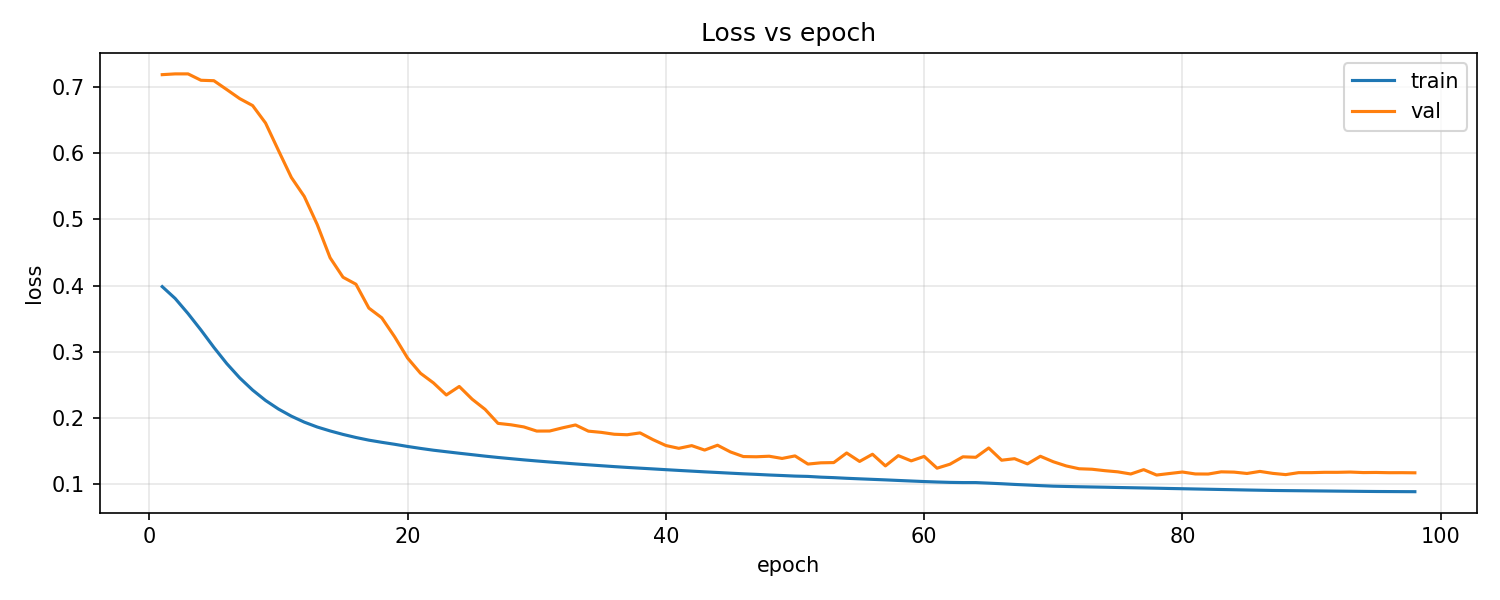
\includegraphics[width=\linewidth]{sae_loss.png}\caption{Perdas.}\end{subfigure}
\begin{subfigure}{.49\textwidth}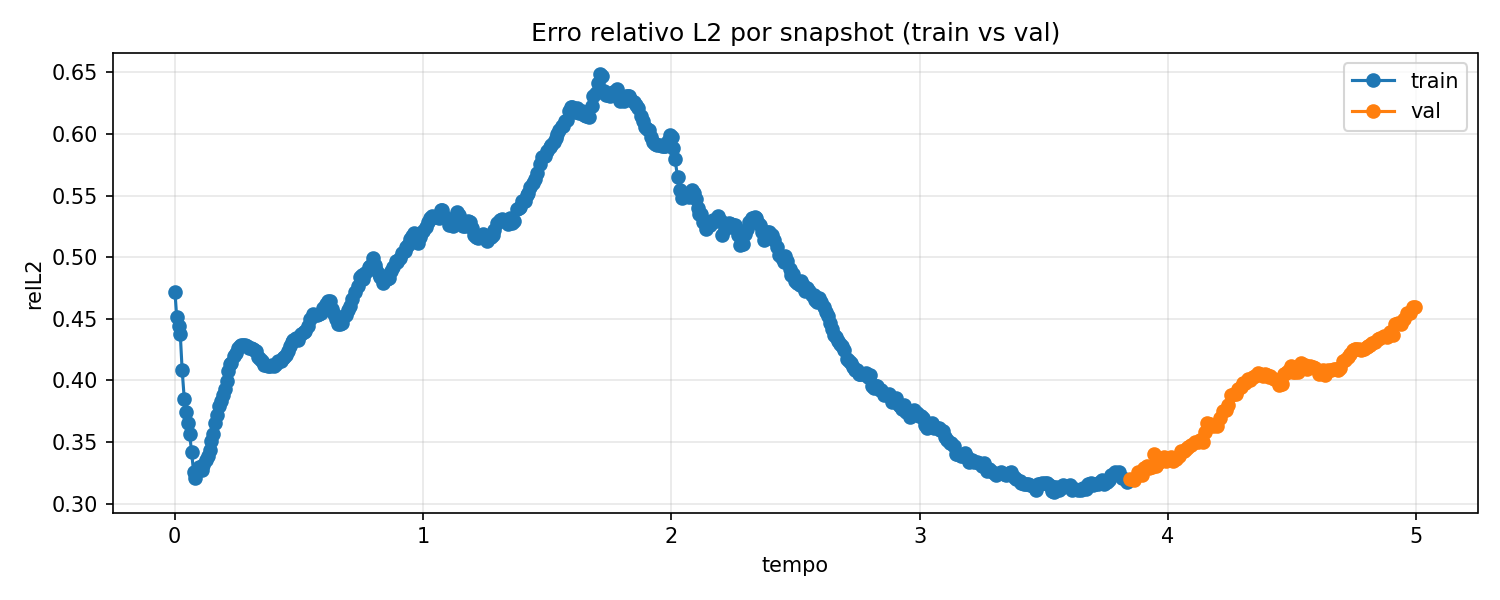
\includegraphics[width=\linewidth]{sae_rel.png}\caption{Erro por snapshot.}\end{subfigure}
\caption{Treinamento e reconstrução SAE.}\end{figure}
\begin{figure}[H]\centering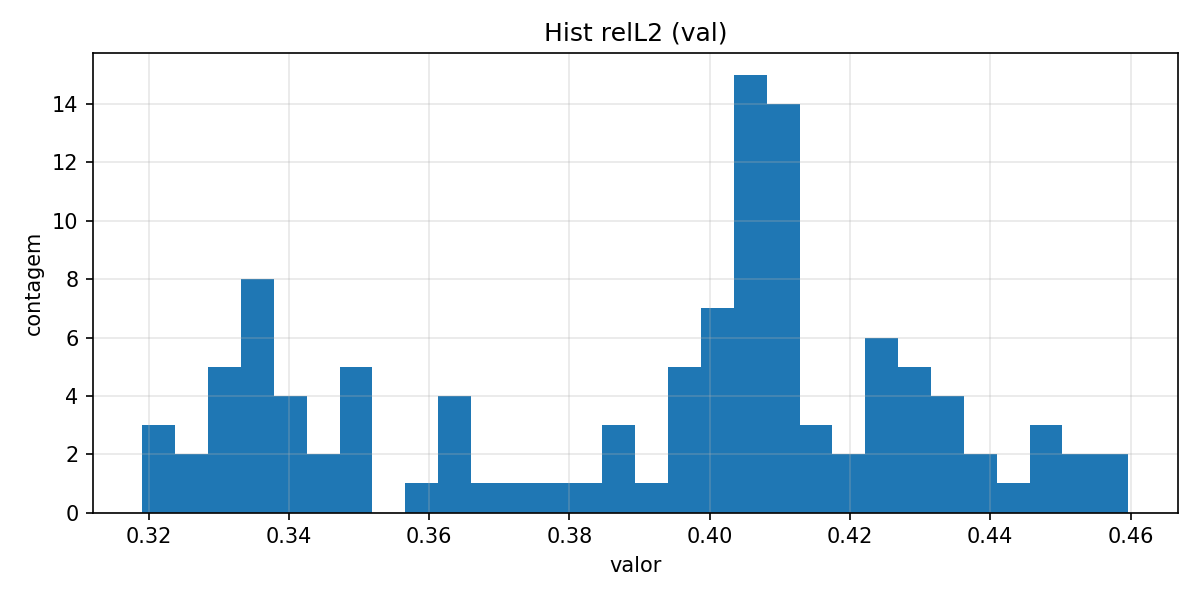
\includegraphics[width=.62\textwidth]{sae_hist.png}\caption{Distribuição do erro de validação.}\end{figure}
\begin{figure}[H]\centering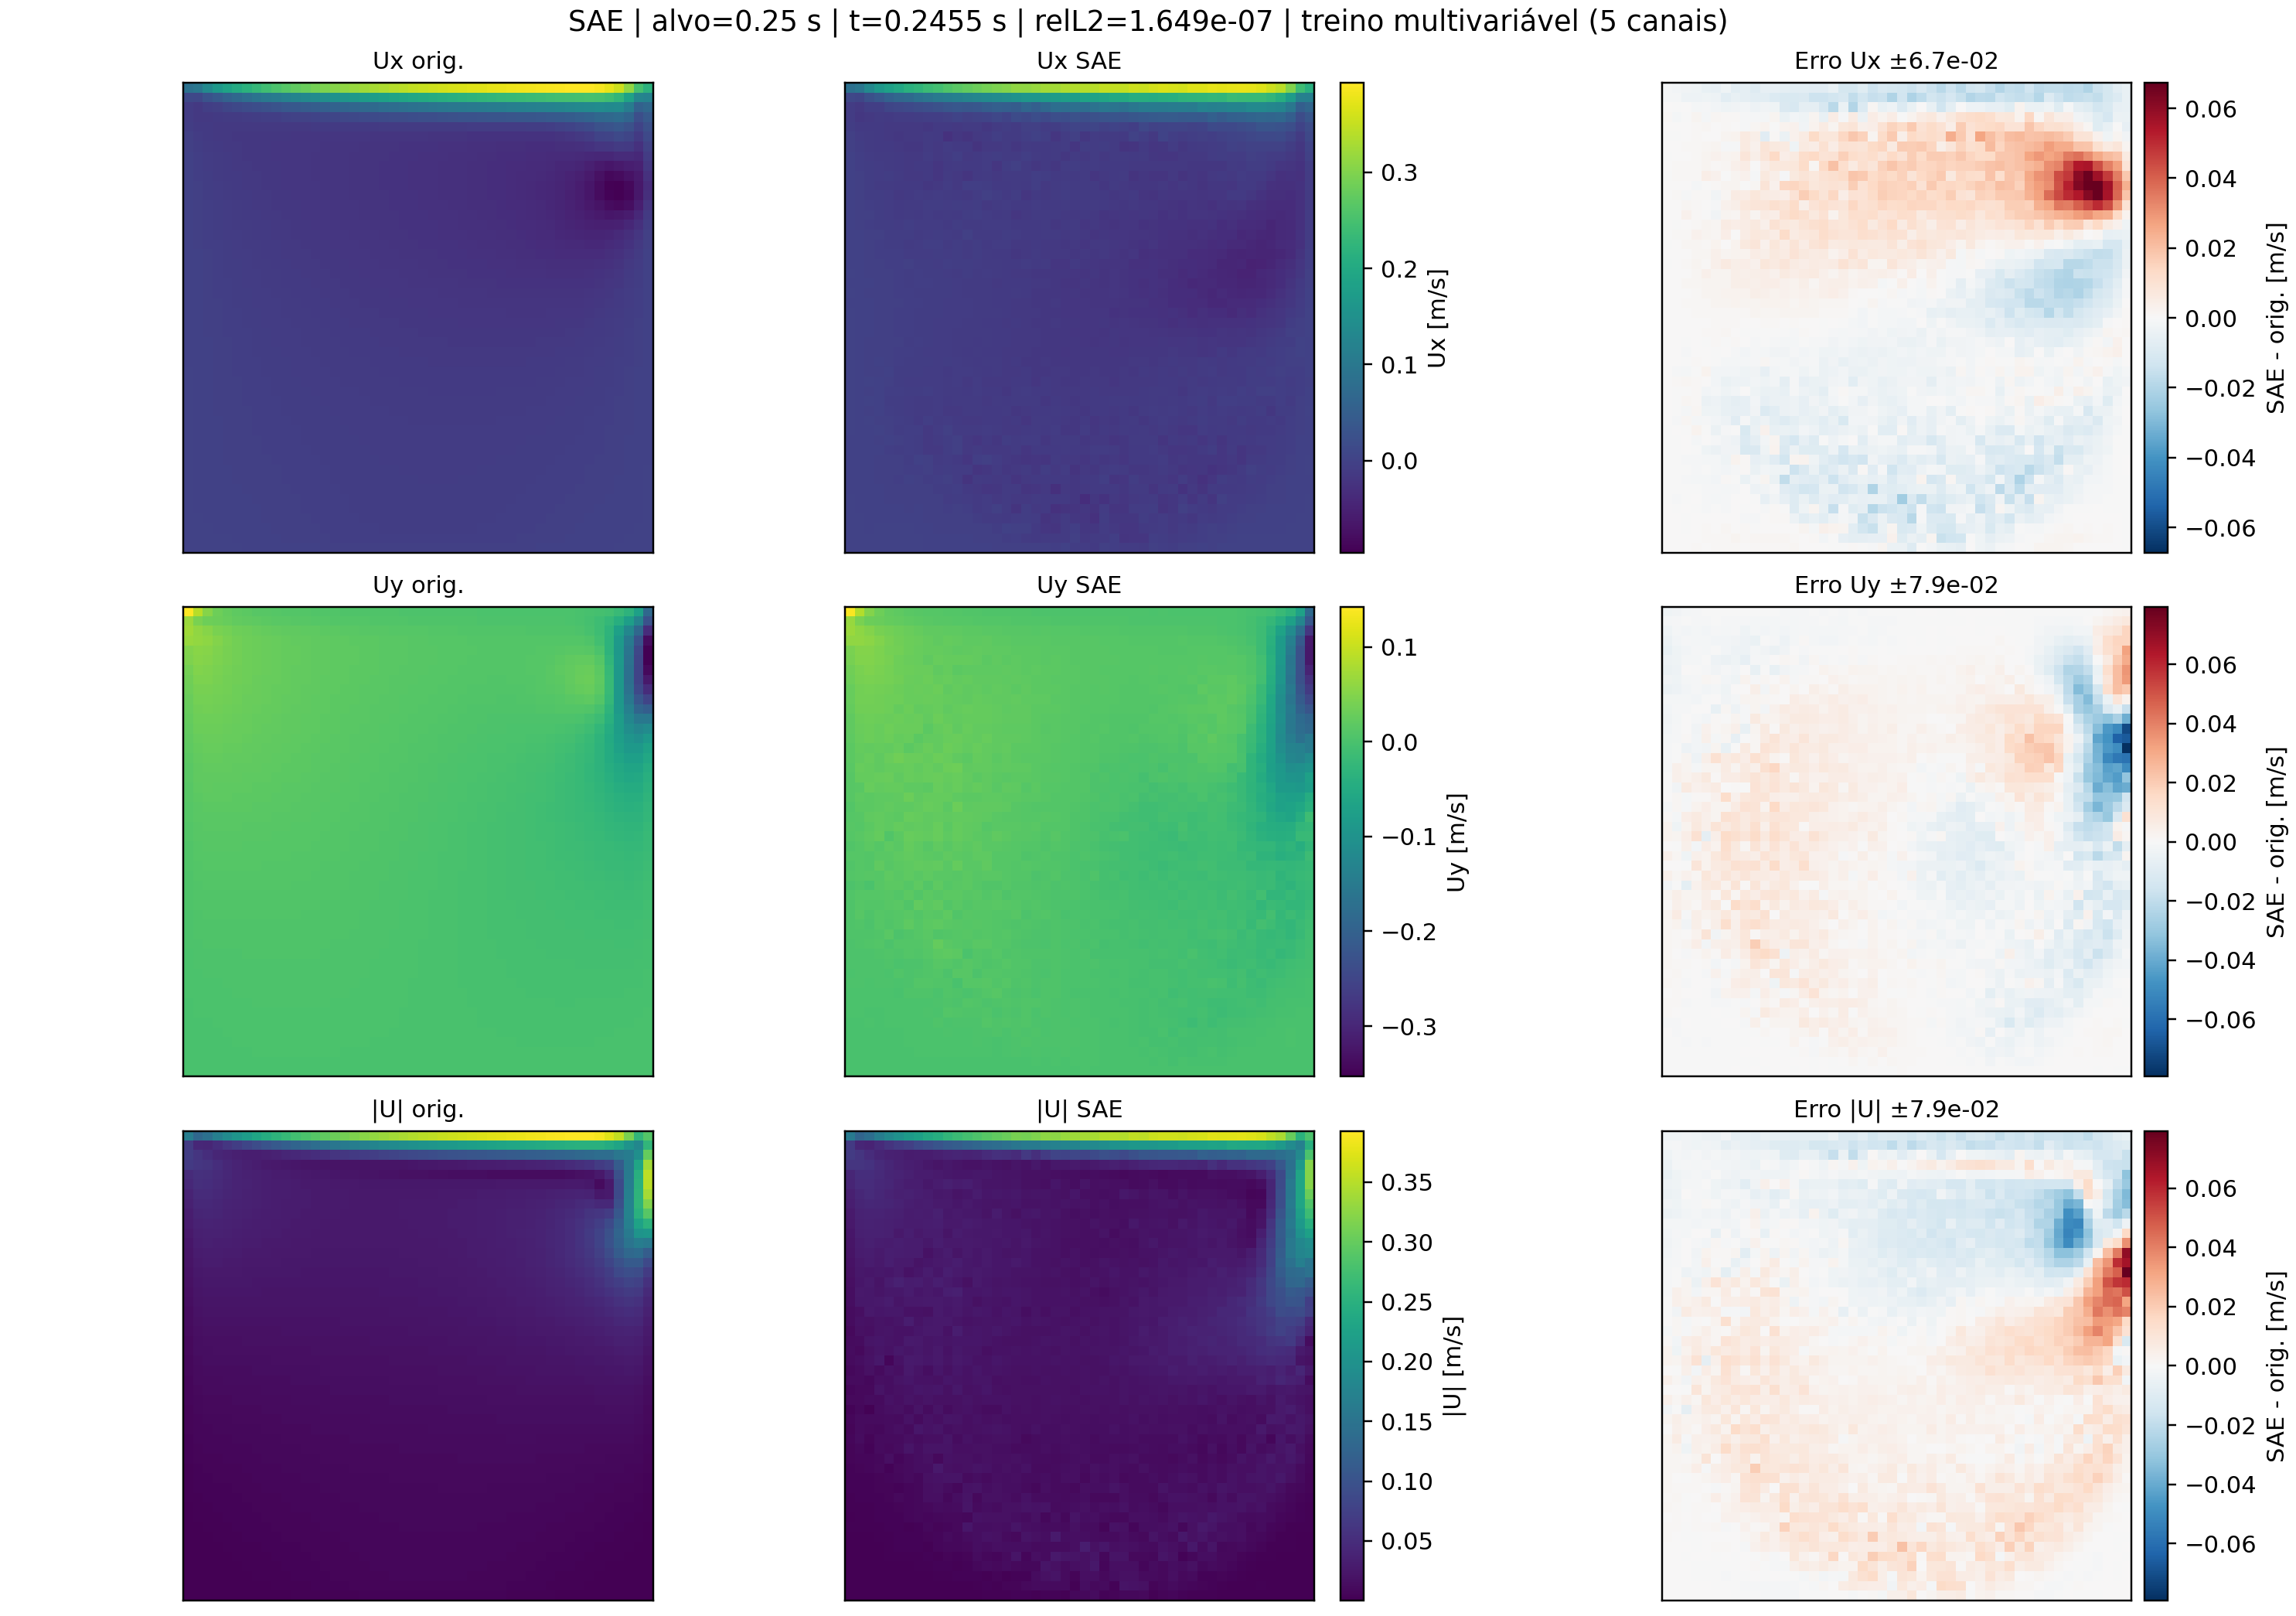
\includegraphics[width=.91\textwidth]{sae_t025.png}\caption{Reconstrução SAE em $t\approx0,25\,\si{s}$.}\end{figure}
\begin{figure}[H]\centering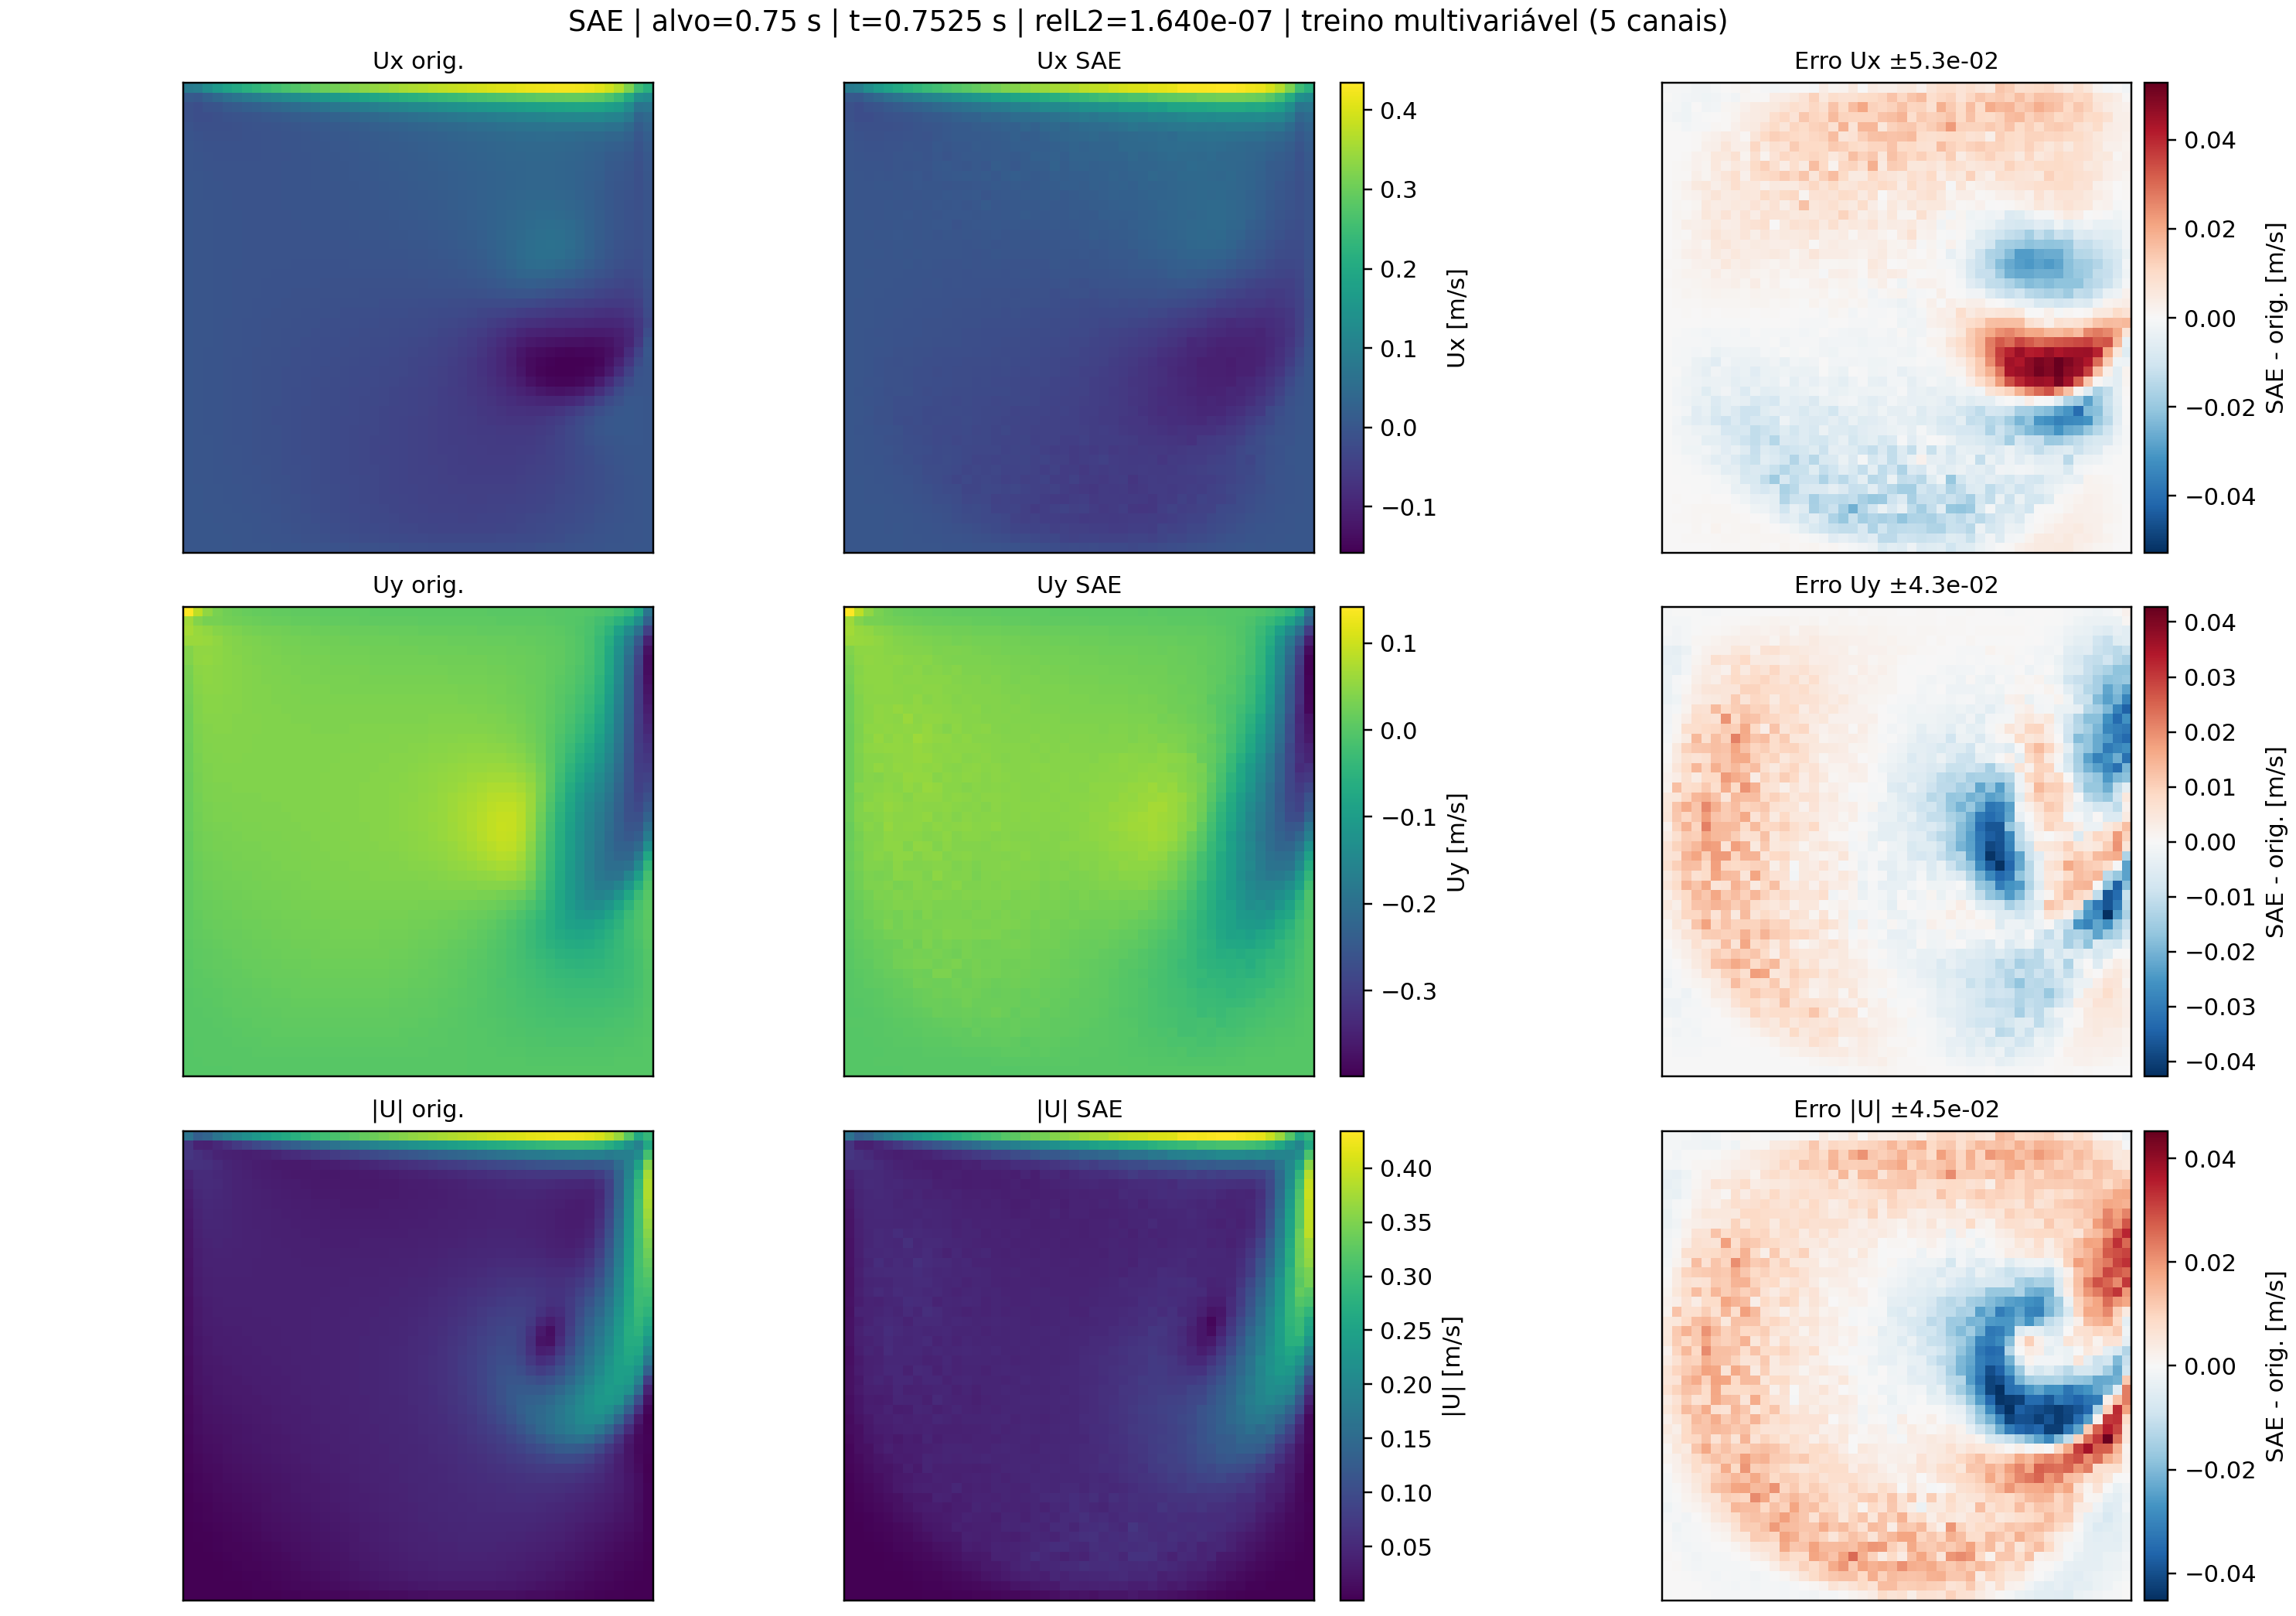
\includegraphics[width=.91\textwidth]{sae_t075.png}\caption{Reconstrução SAE em $t\approx0,75\,\si{s}$.}\end{figure}

POD e SAE isolados apenas constroem representações e reconstroem snapshots. Eles não definem $dq/dt$ e, portanto, não capturam dinâmica por si mesmos.

\section{Identificação dinâmica SINDy}
SINDy ajusta $\dot q=\Theta(q,t)\Xi$. A integração livre, sem consultar estados verdadeiros futuros, é o principal teste dinâmico.

\subsection{POD--SINDy}
O modelo principal usa oito coordenadas (98,65\% de energia), biblioteca polinomial de ordem 2, sem seno, 45 funções e Lasso $\alpha=0,1$. Há 16 coeficientes não nulos em 360. O erro de derivada é 0,64138. A integração livre falha; o erro 1,39886 vem de fallback de um passo guiado e não é erro de previsão autônoma.
\lstinputlisting[style=sindyeq,caption={Equações completas POD--SINDy.}]{equacoes_pod_sindy.txt}
\begin{figure}[H]\centering
\begin{subfigure}{.49\textwidth}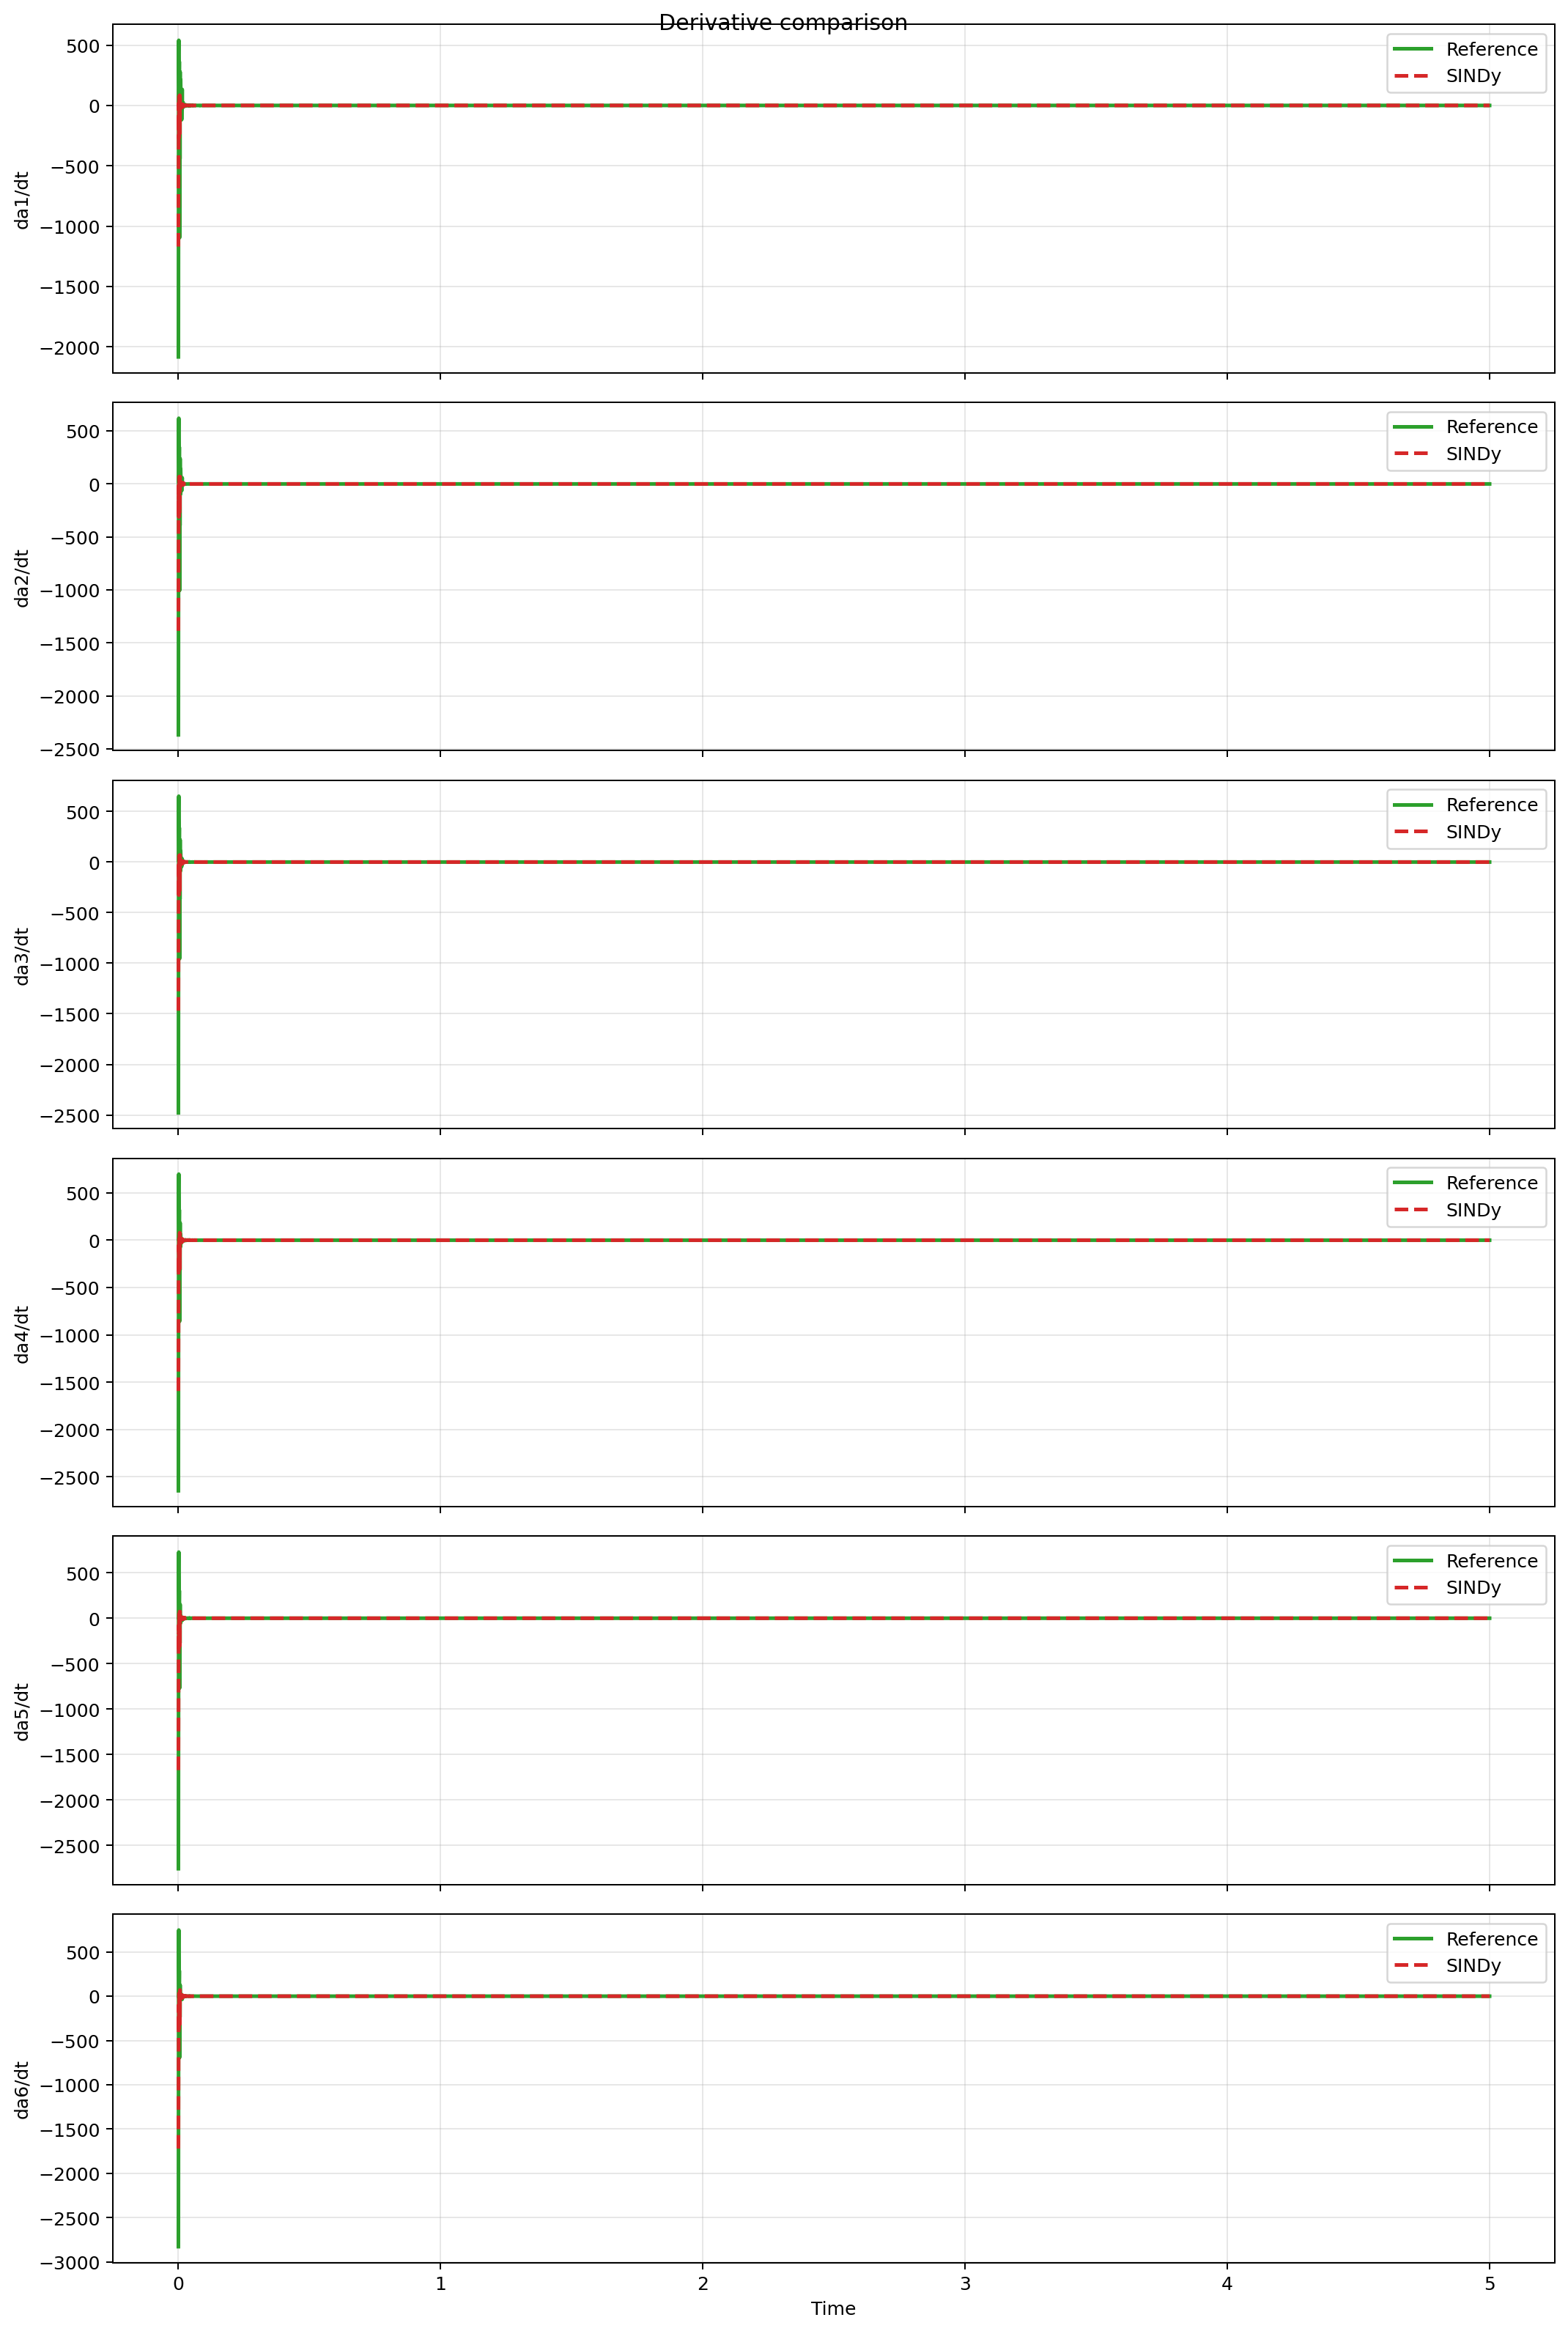
\includegraphics[width=\linewidth]{pods_deriv.png}\caption{Derivadas.}\end{subfigure}
\begin{subfigure}{.49\textwidth}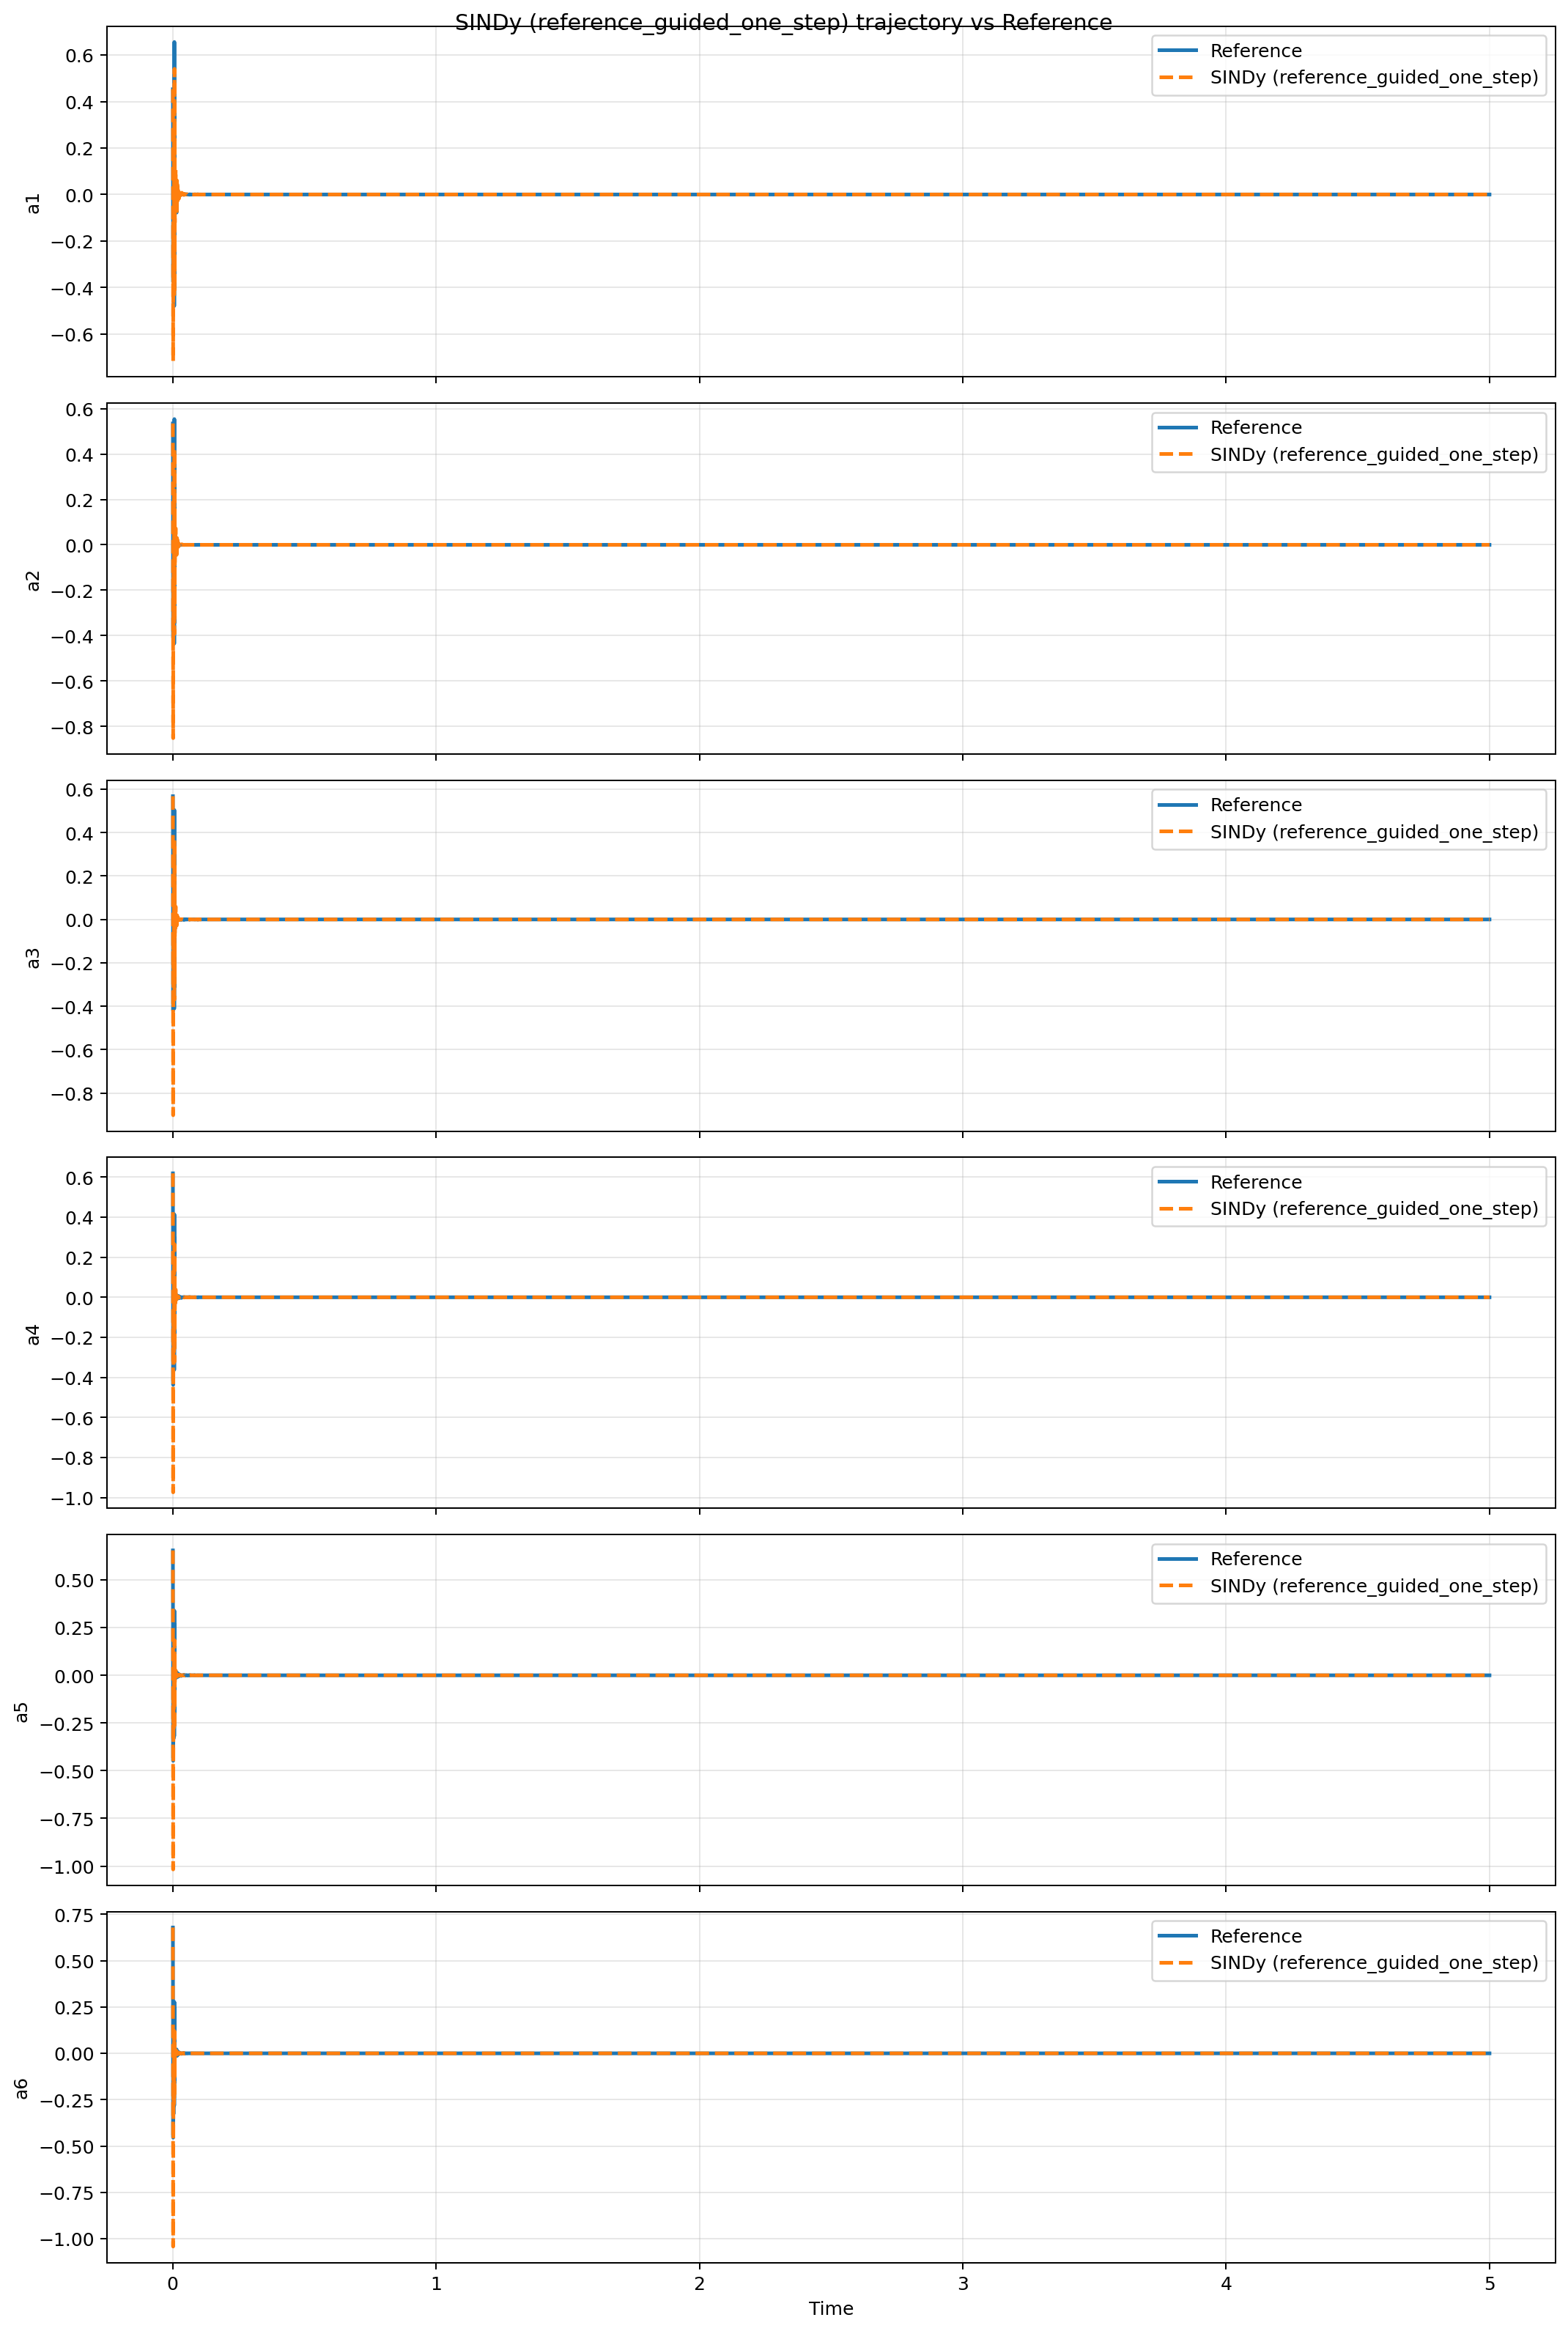
\includegraphics[width=\linewidth]{pods_traj.png}\caption{Fallback guiado.}\end{subfigure}
\caption{POD--SINDy principal.}\end{figure}
\begin{figure}[H]\centering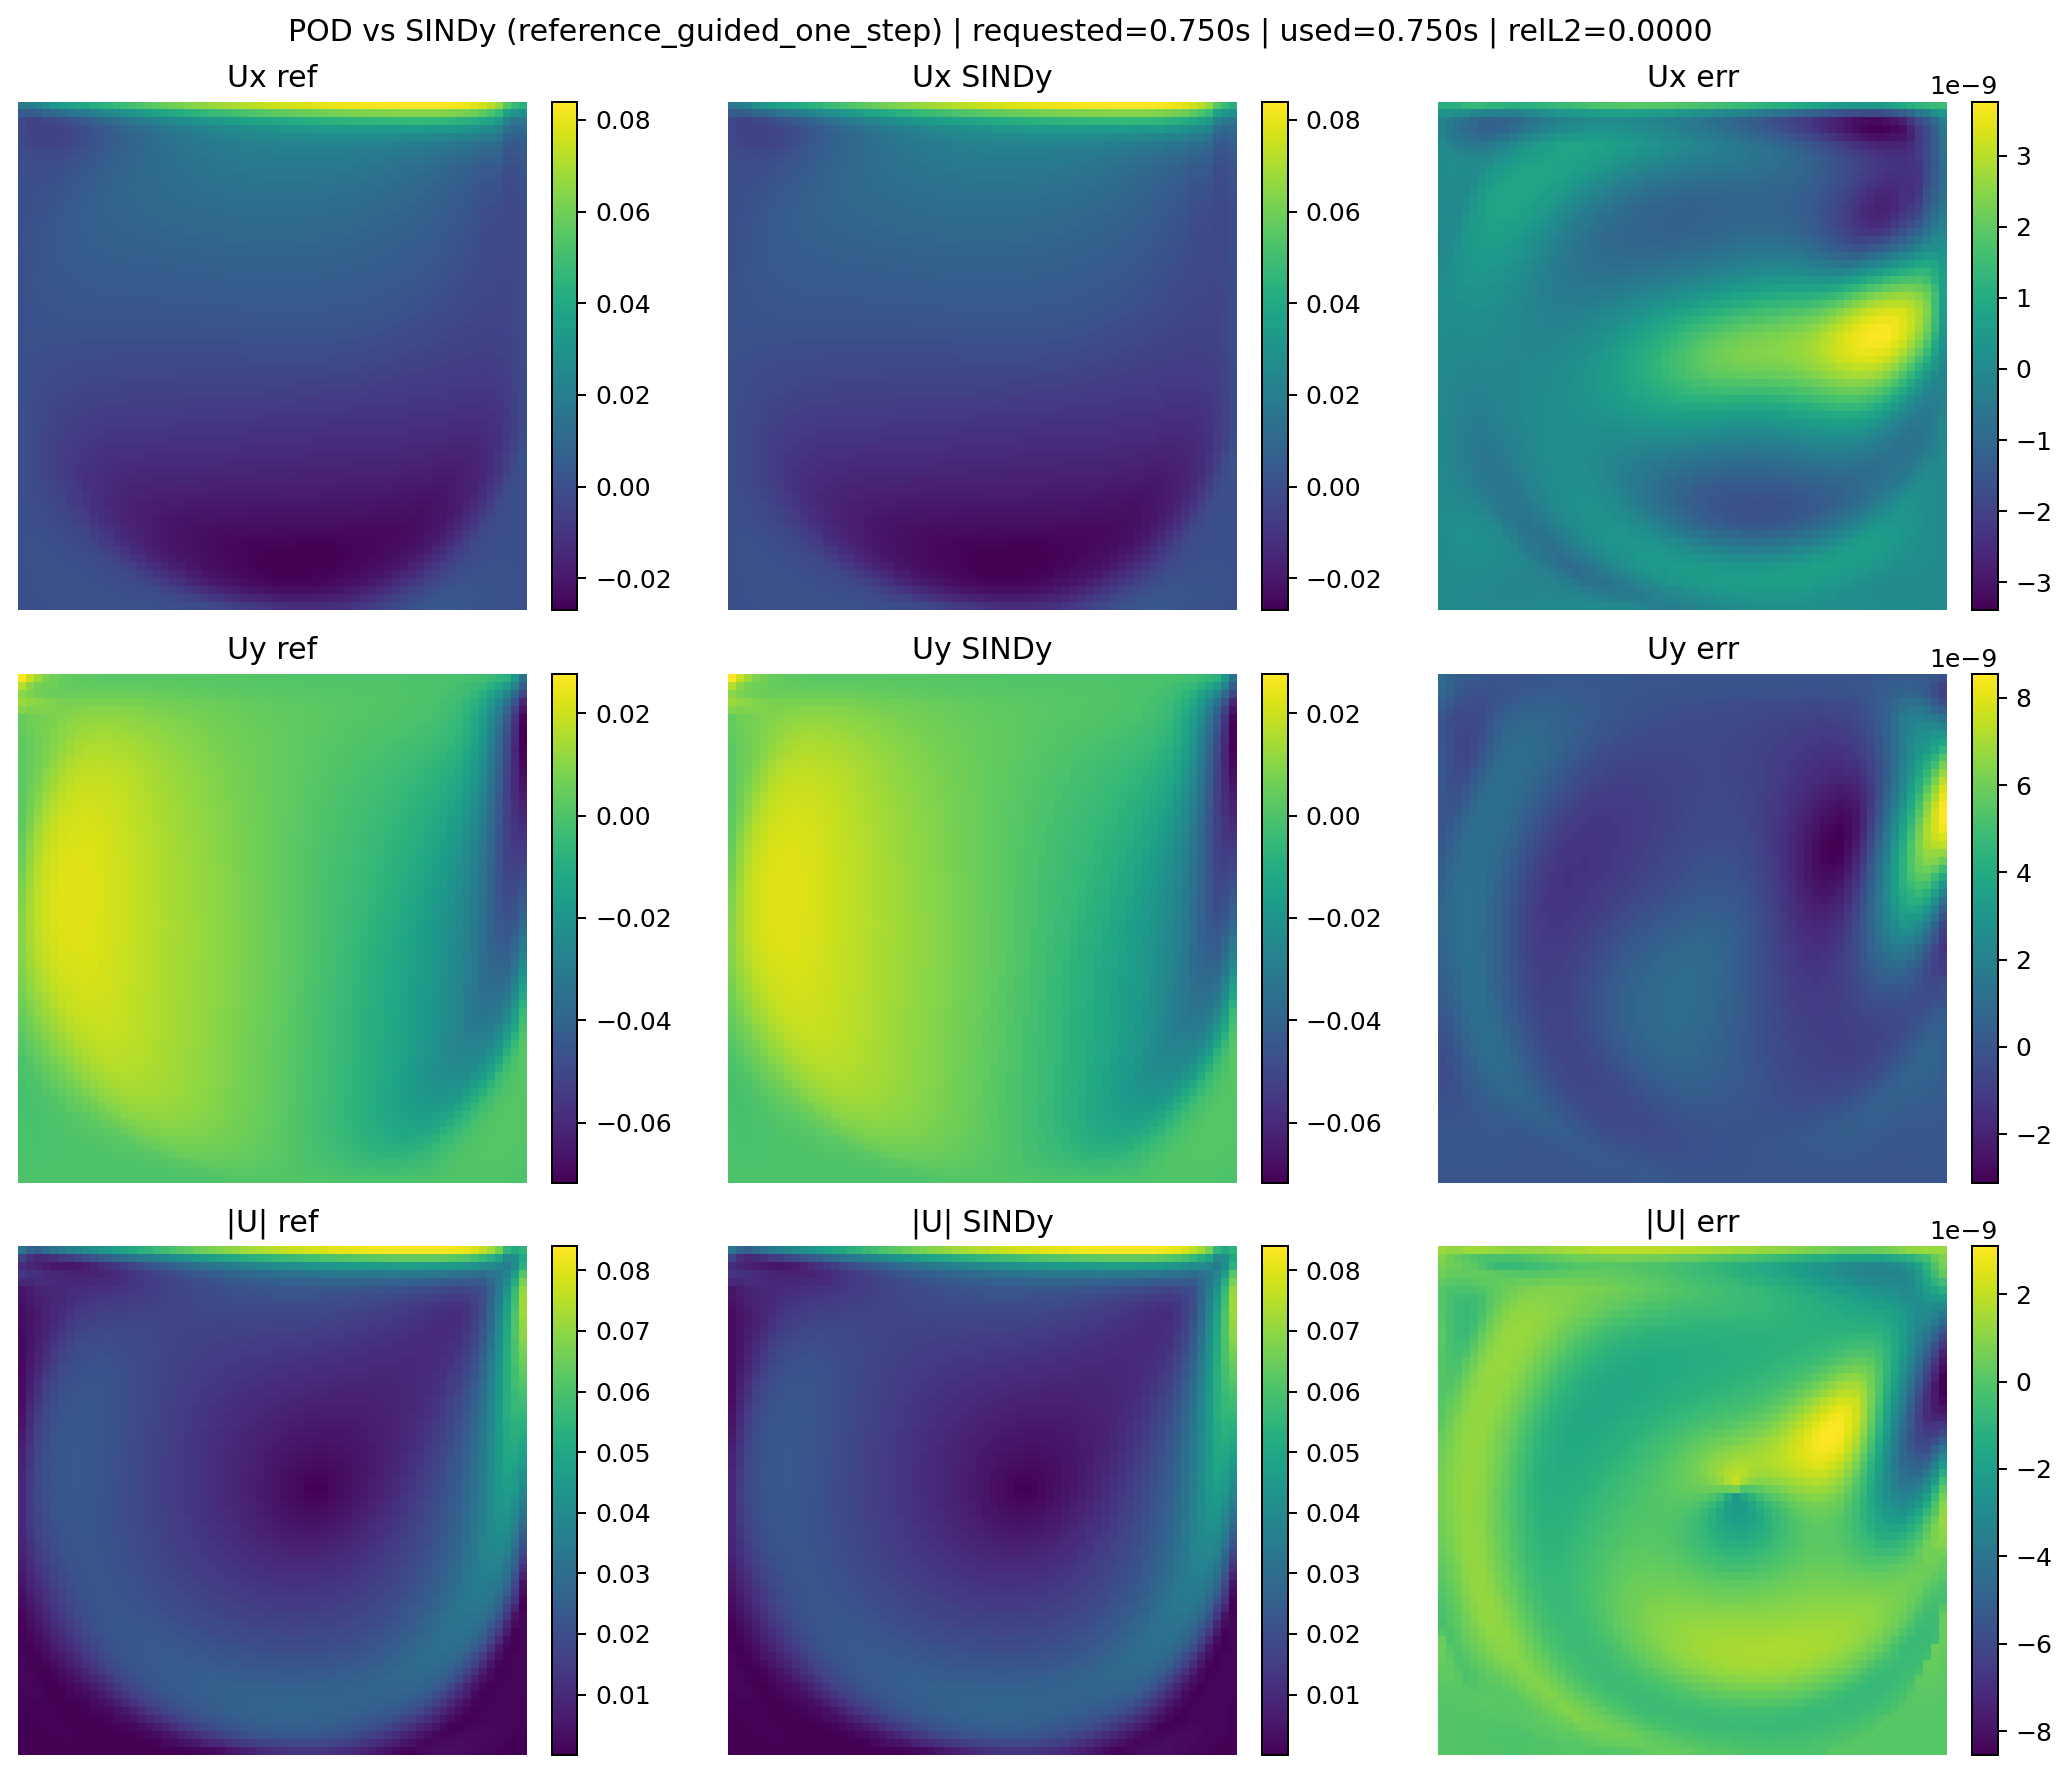
\includegraphics[width=.89\textwidth]{pods_t075.png}\caption{Reconstrução POD--SINDy próxima de $t=0,75\,\si{s}$; dois canais da POD são inválidos.}\end{figure}

A busca de 84 alternativas não aceitou nenhuma. O melhor compromisso usa 16 modos, 99,872\% da energia, ordem 1 com seno, $\alpha=0,1$ e 16 termos em 784. A integração livre termina, mas o erro é 3,1405, pior que o modelo principal guiado.

\subsubsection{Reexecução com a POD corrigida}
Com oito modos corretos, a energia é 99,303\%. O melhor ajuste principal usa ordem 2, sem seno e $\alpha=10^{-4}$: erro de derivada 0,07290 e 118 termos não nulos em 360. Apesar da melhora local expressiva, a integração livre ainda falha; o erro 0,000136 é somente do fallback guiado.

Na busca de 84 modelos, 56 passam pelos limites locais. O escolhido usa 16 modos (99,886\% de energia), ordem 2 com seno, $\alpha=0,01$ e 30 termos em 2960. Seu erro de derivada é 0,7633 e o erro guiado é 0,001554, mas a integração livre também falha. Logo, corrigir os campos melhora projeção e ajuste local, porém não resolve a estabilidade dinâmica.
\lstinputlisting[style=sindyeq,caption={Equações POD--SINDy após correção dos campos.}]{equacoes_pod_sindy_corrigido.txt}
\begin{figure}[H]\centering
\begin{subfigure}{.49\textwidth}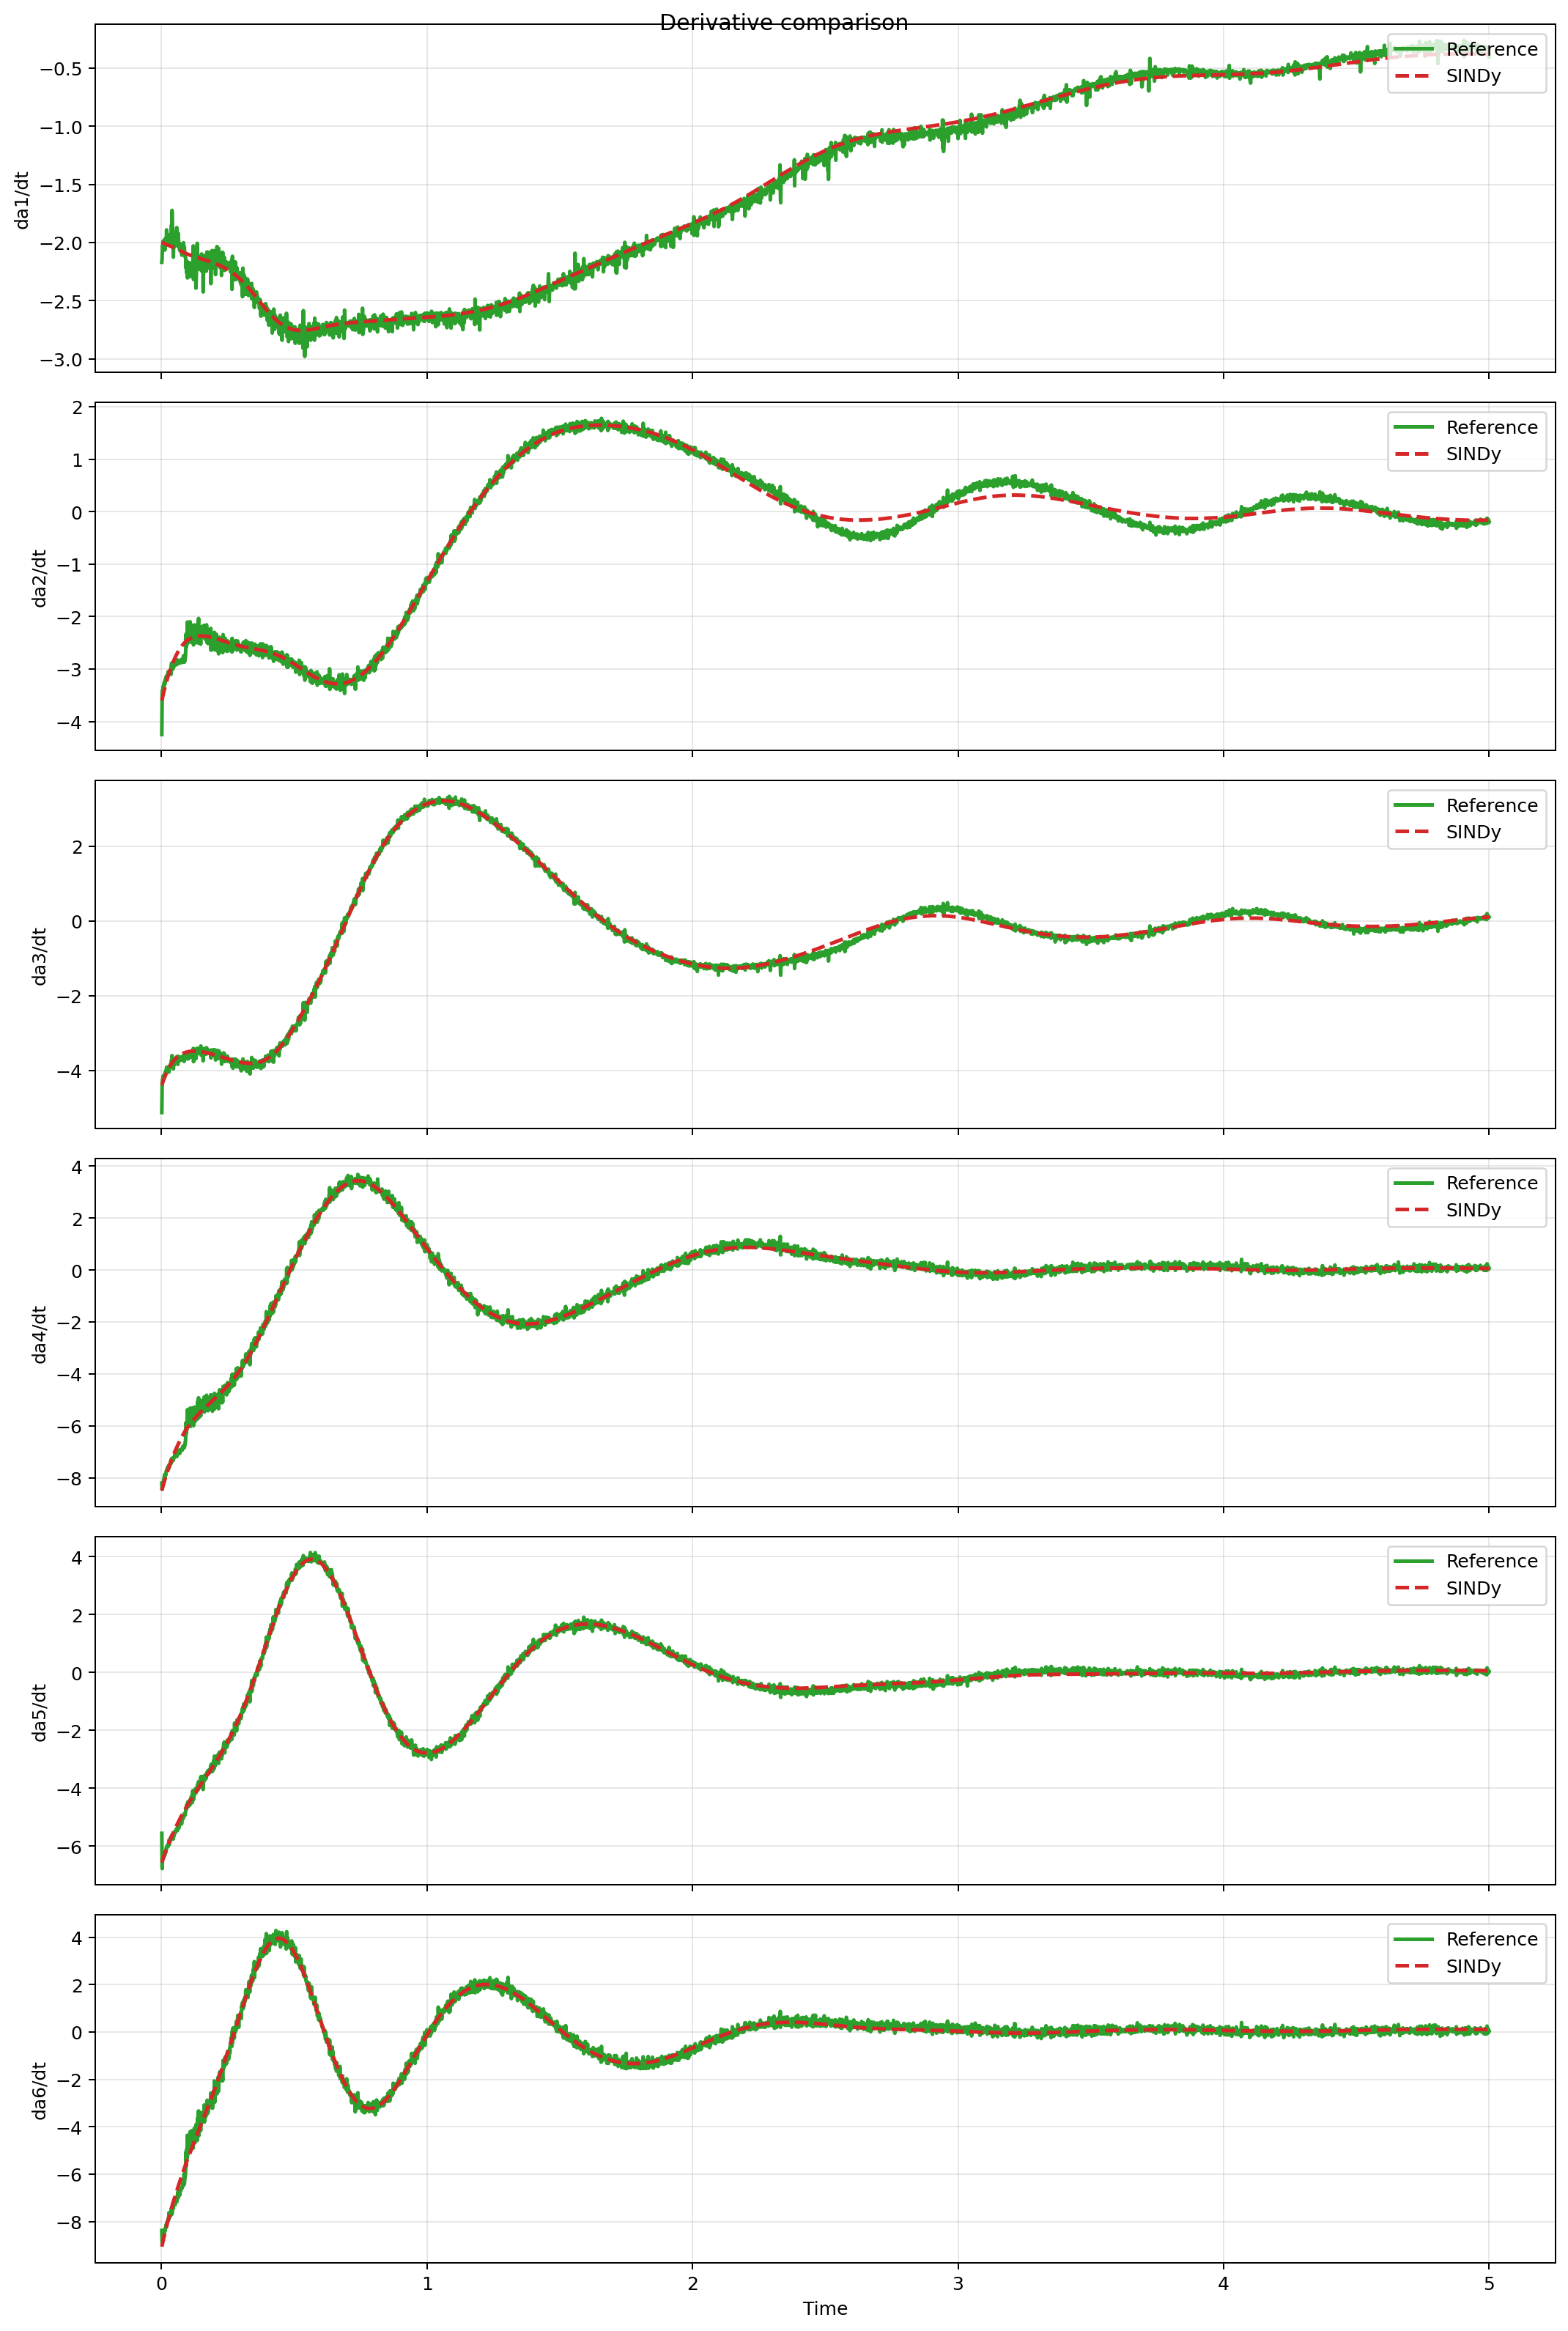
\includegraphics[width=\linewidth]{pods_corr_deriv.png}\caption{Derivadas corrigidas.}\end{subfigure}
\begin{subfigure}{.49\textwidth}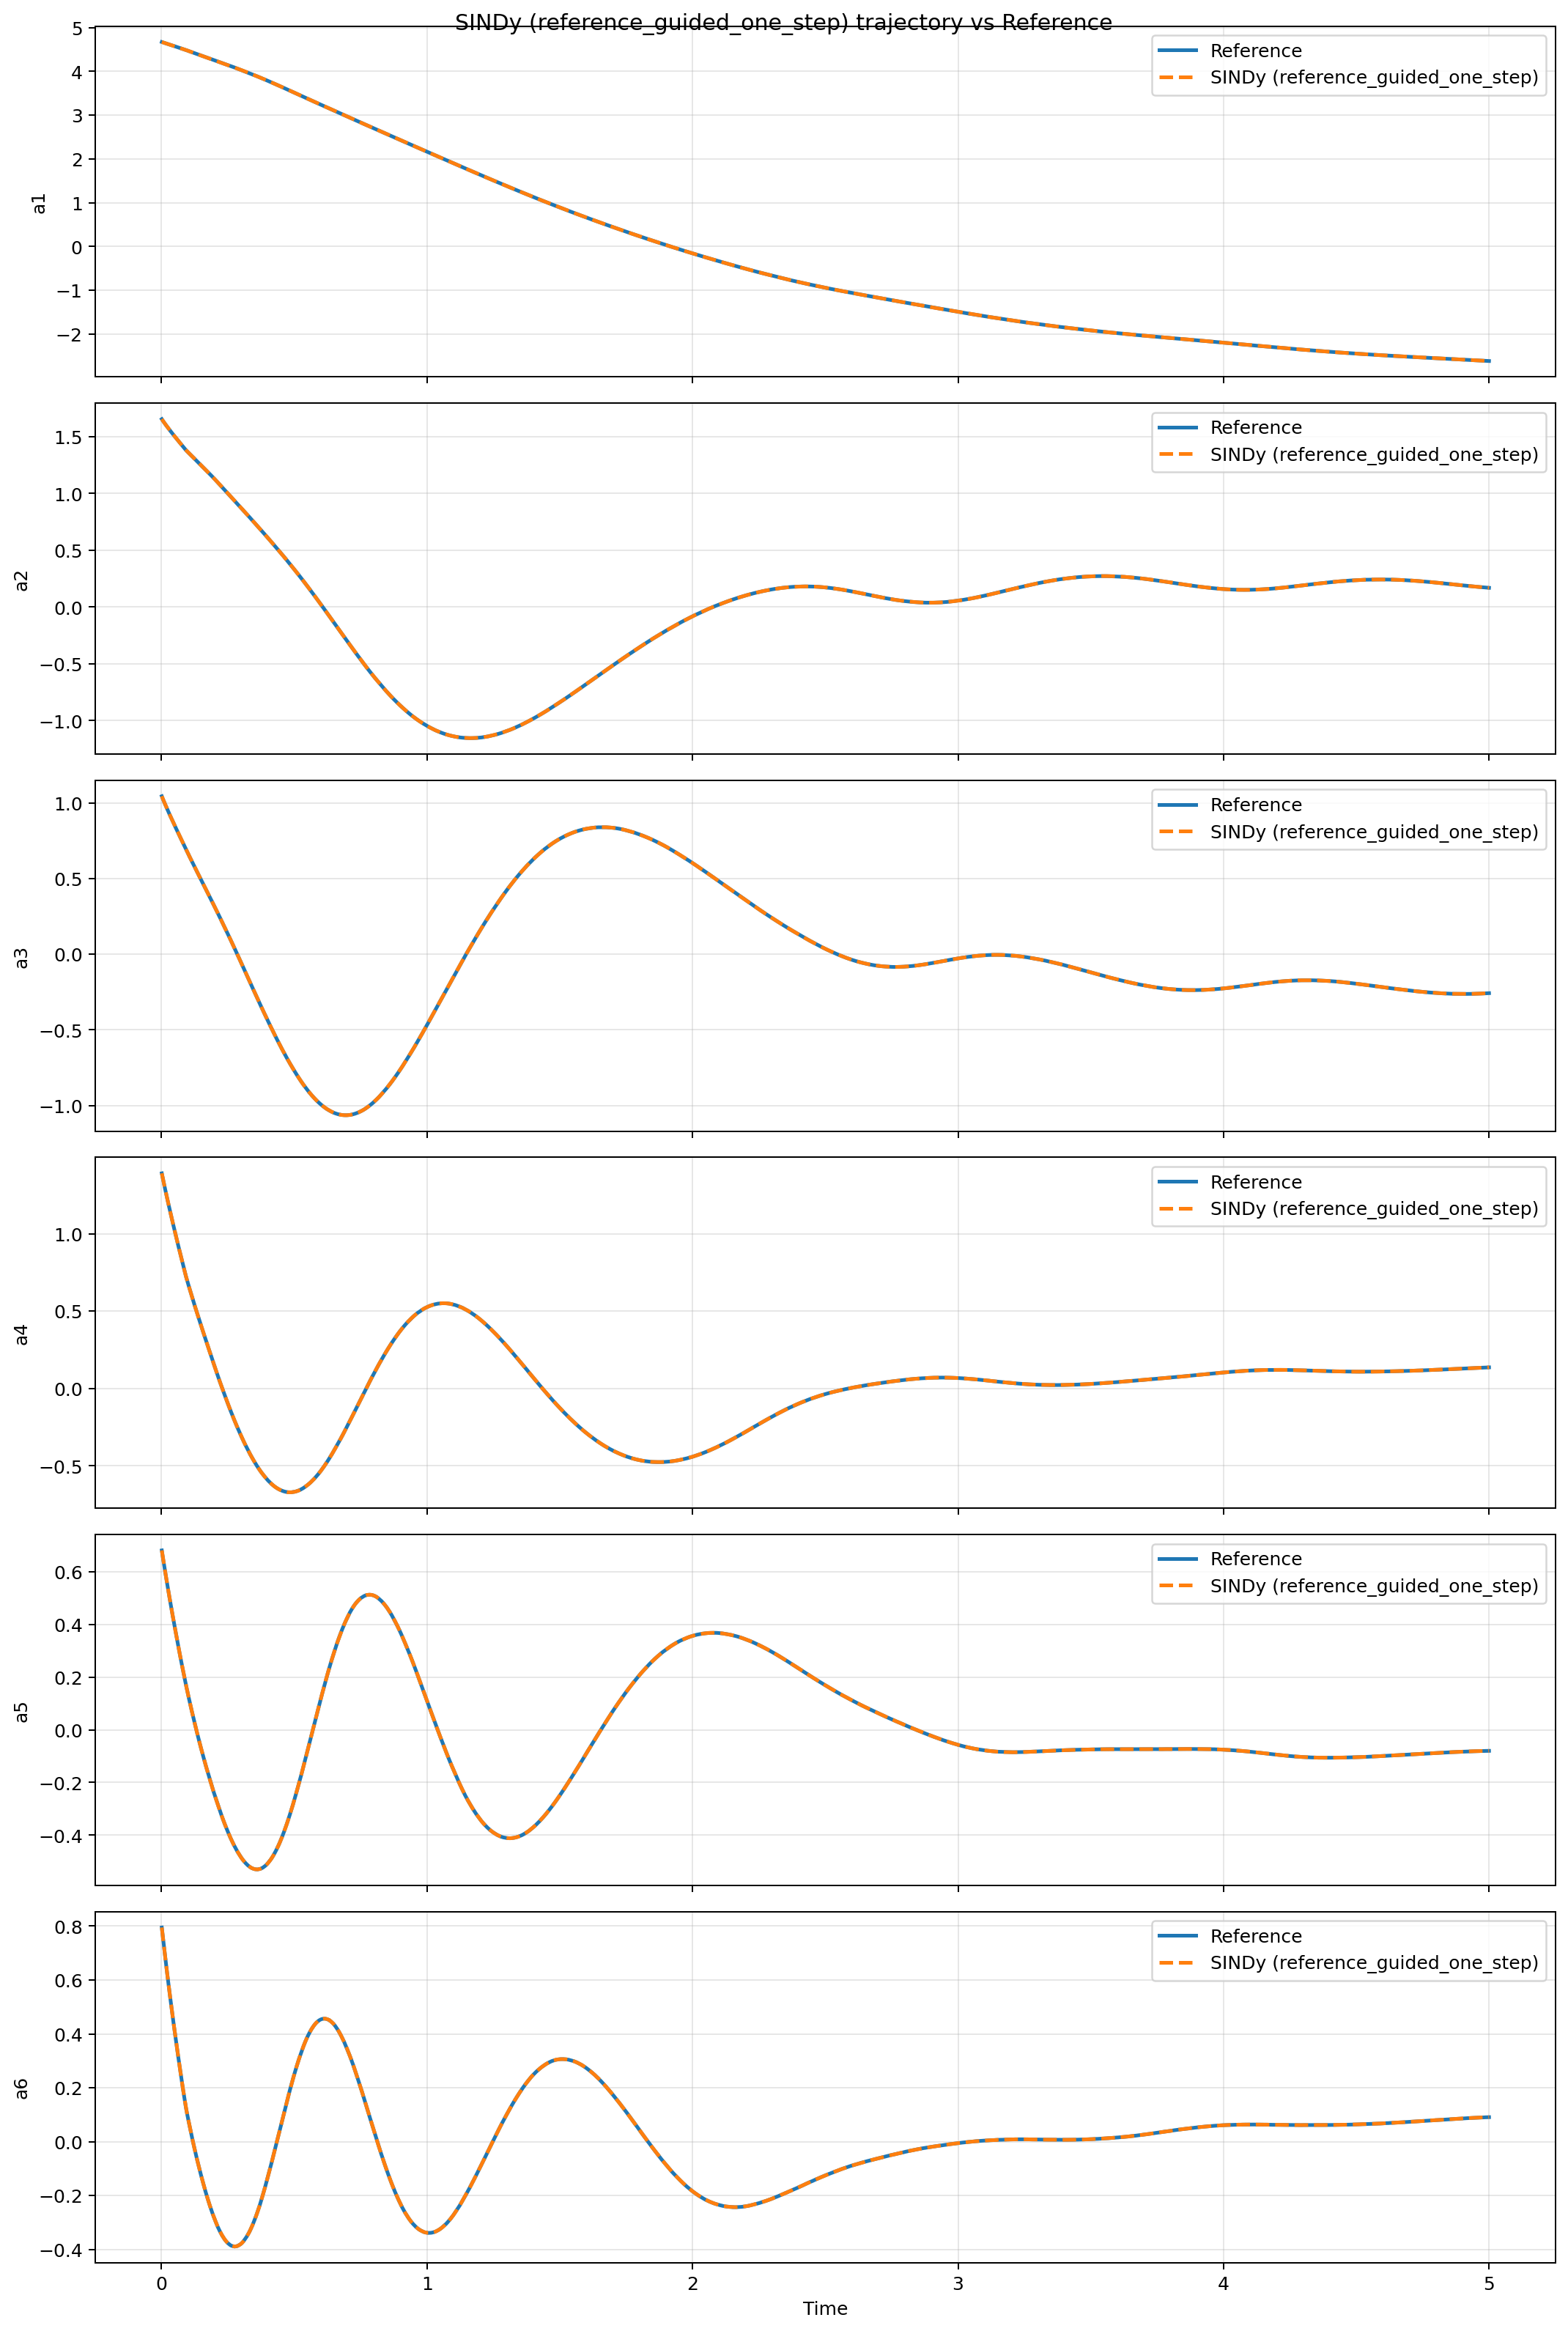
\includegraphics[width=\linewidth]{pods_corr_traj.png}\caption{Fallback guiado corrigido.}\end{subfigure}
\caption{POD--SINDy reexecutado com $U_x,U_y,p,T,k$.}\end{figure}

\subsection{SAE--SINDy}
O modelo usa oito latentes, ordem 2, seno/cosseno, 61 funções e $\alpha=10^{-3}$. Mantém 151 de 488 coeficientes. O erro de derivada é 0,61588. A integração livre falha; o erro guiado 0,01768 mede apenas consistência local.
\lstinputlisting[style=sindyeq,caption={Equações completas SAE--SINDy.}]{equacoes_sae_sindy.txt}
\begin{figure}[H]\centering
\begin{subfigure}{.49\textwidth}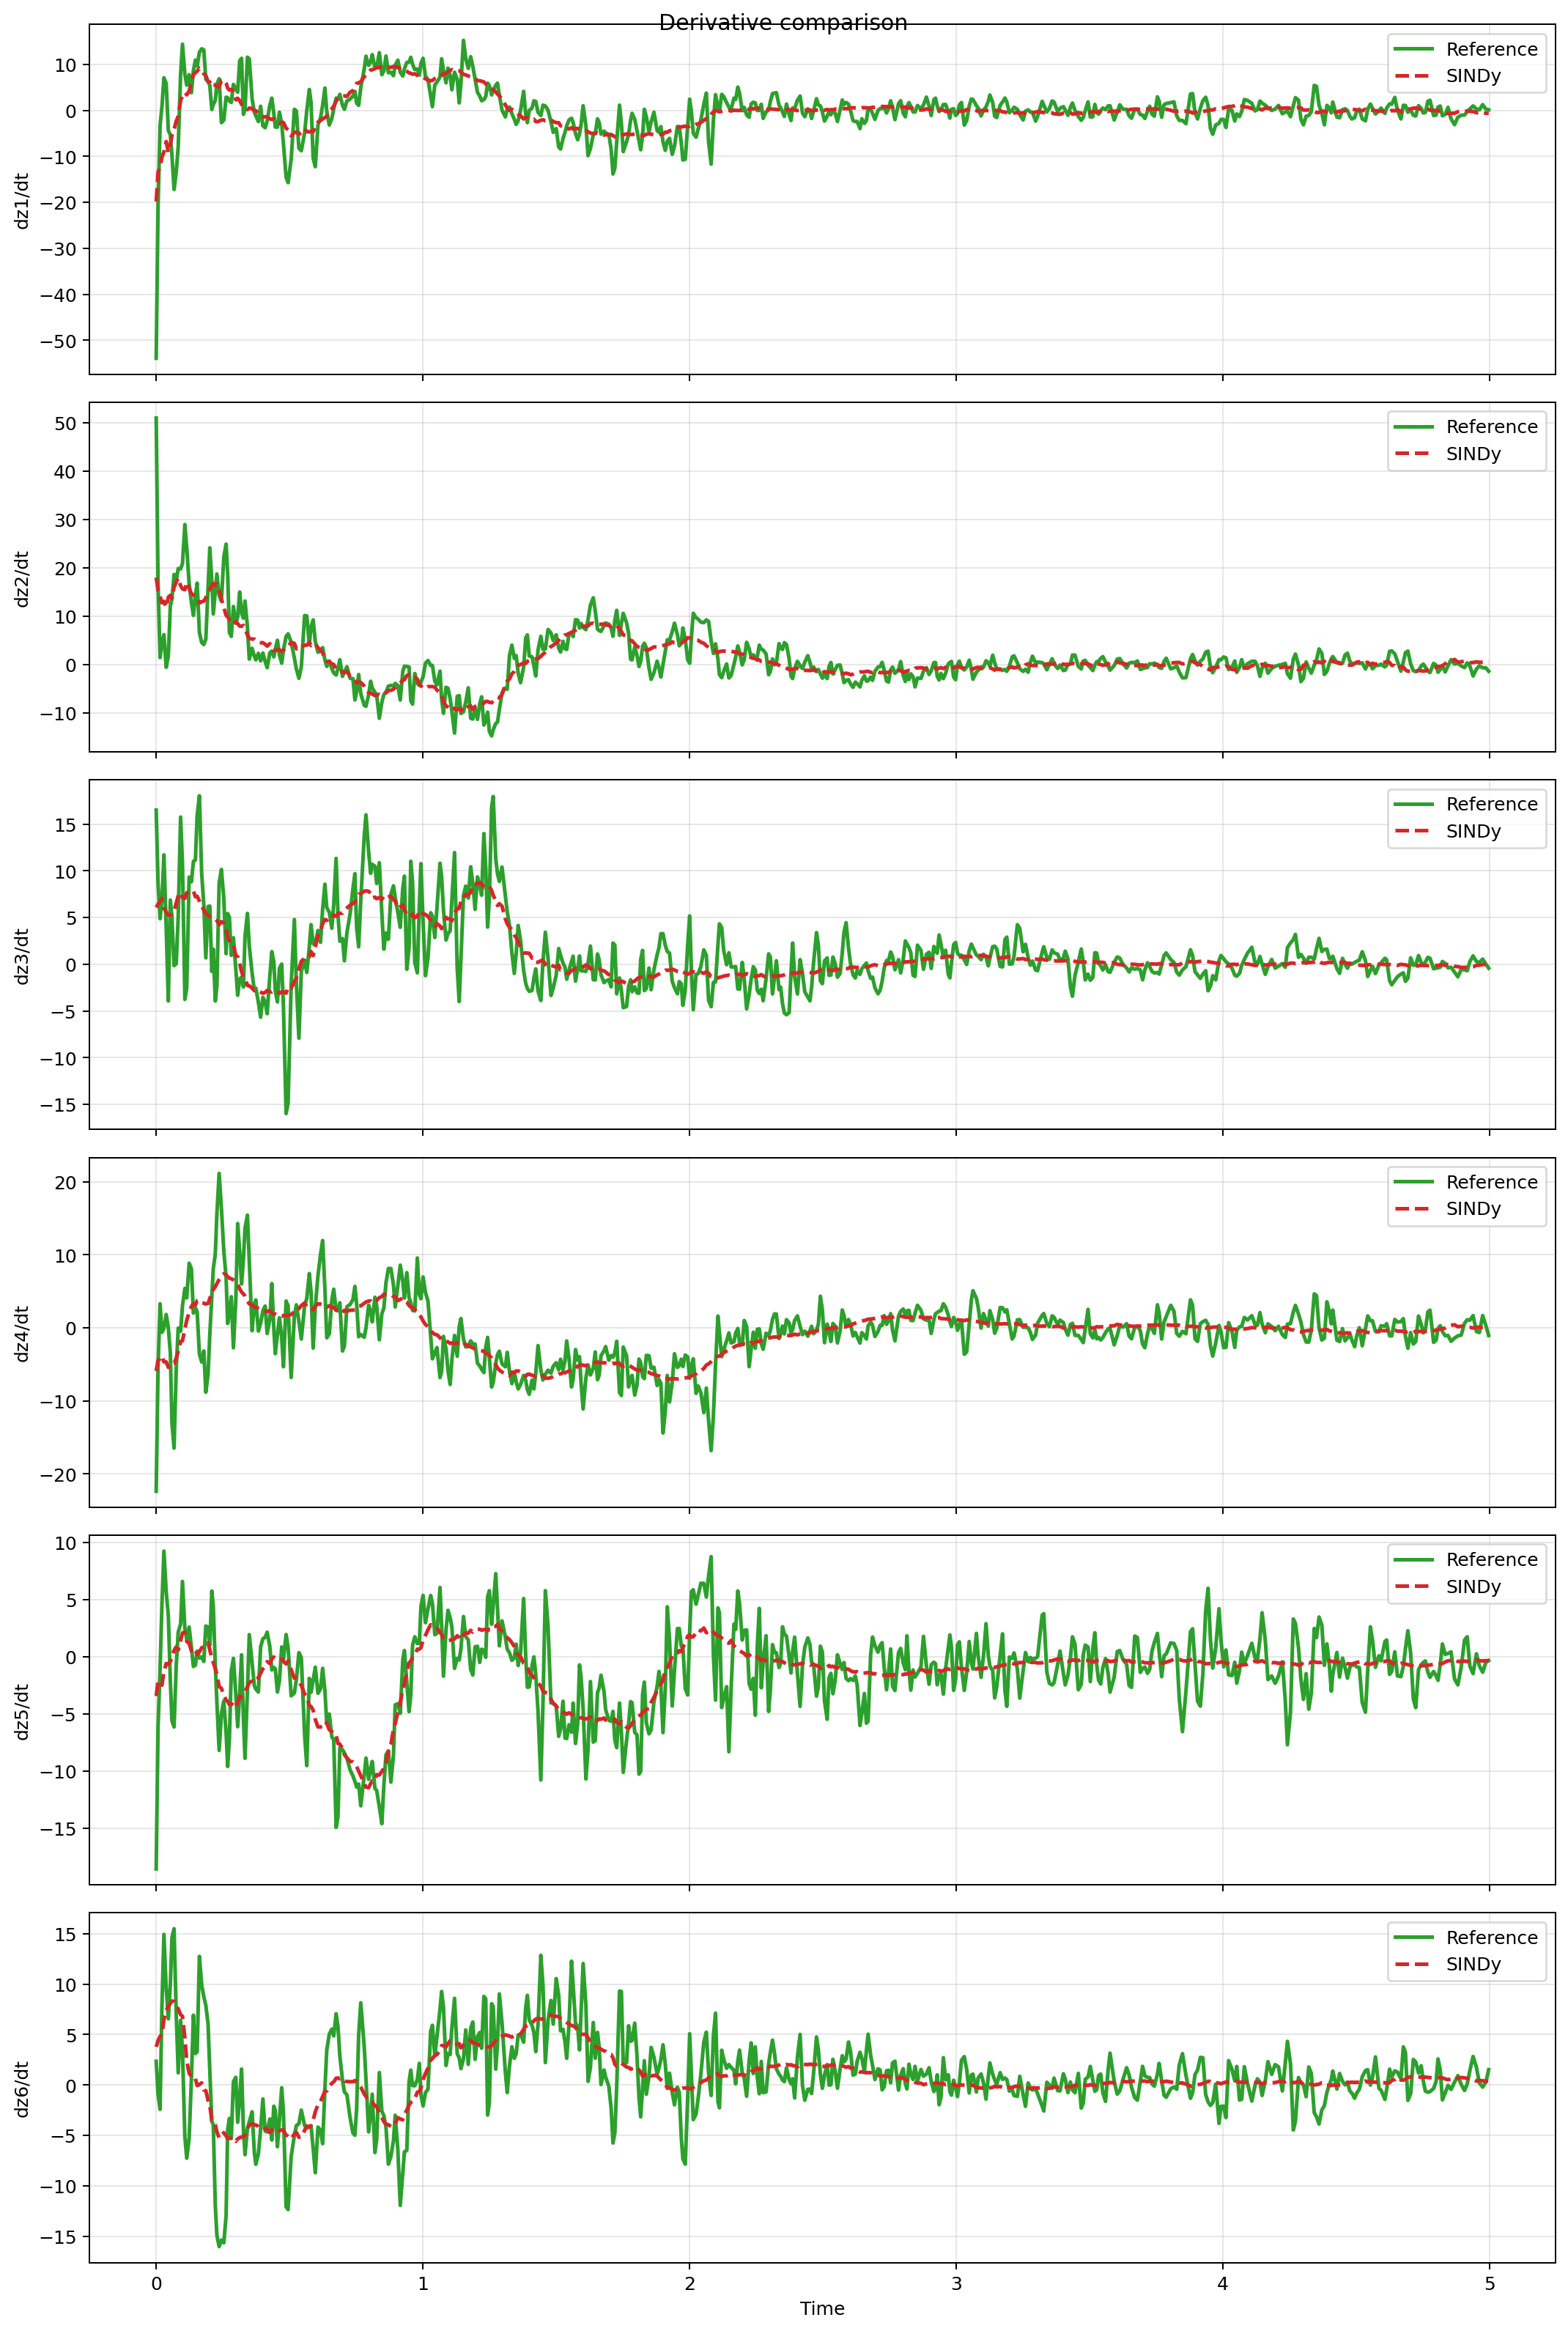
\includegraphics[width=\linewidth]{saes_deriv.png}\caption{Derivadas.}\end{subfigure}
\begin{subfigure}{.49\textwidth}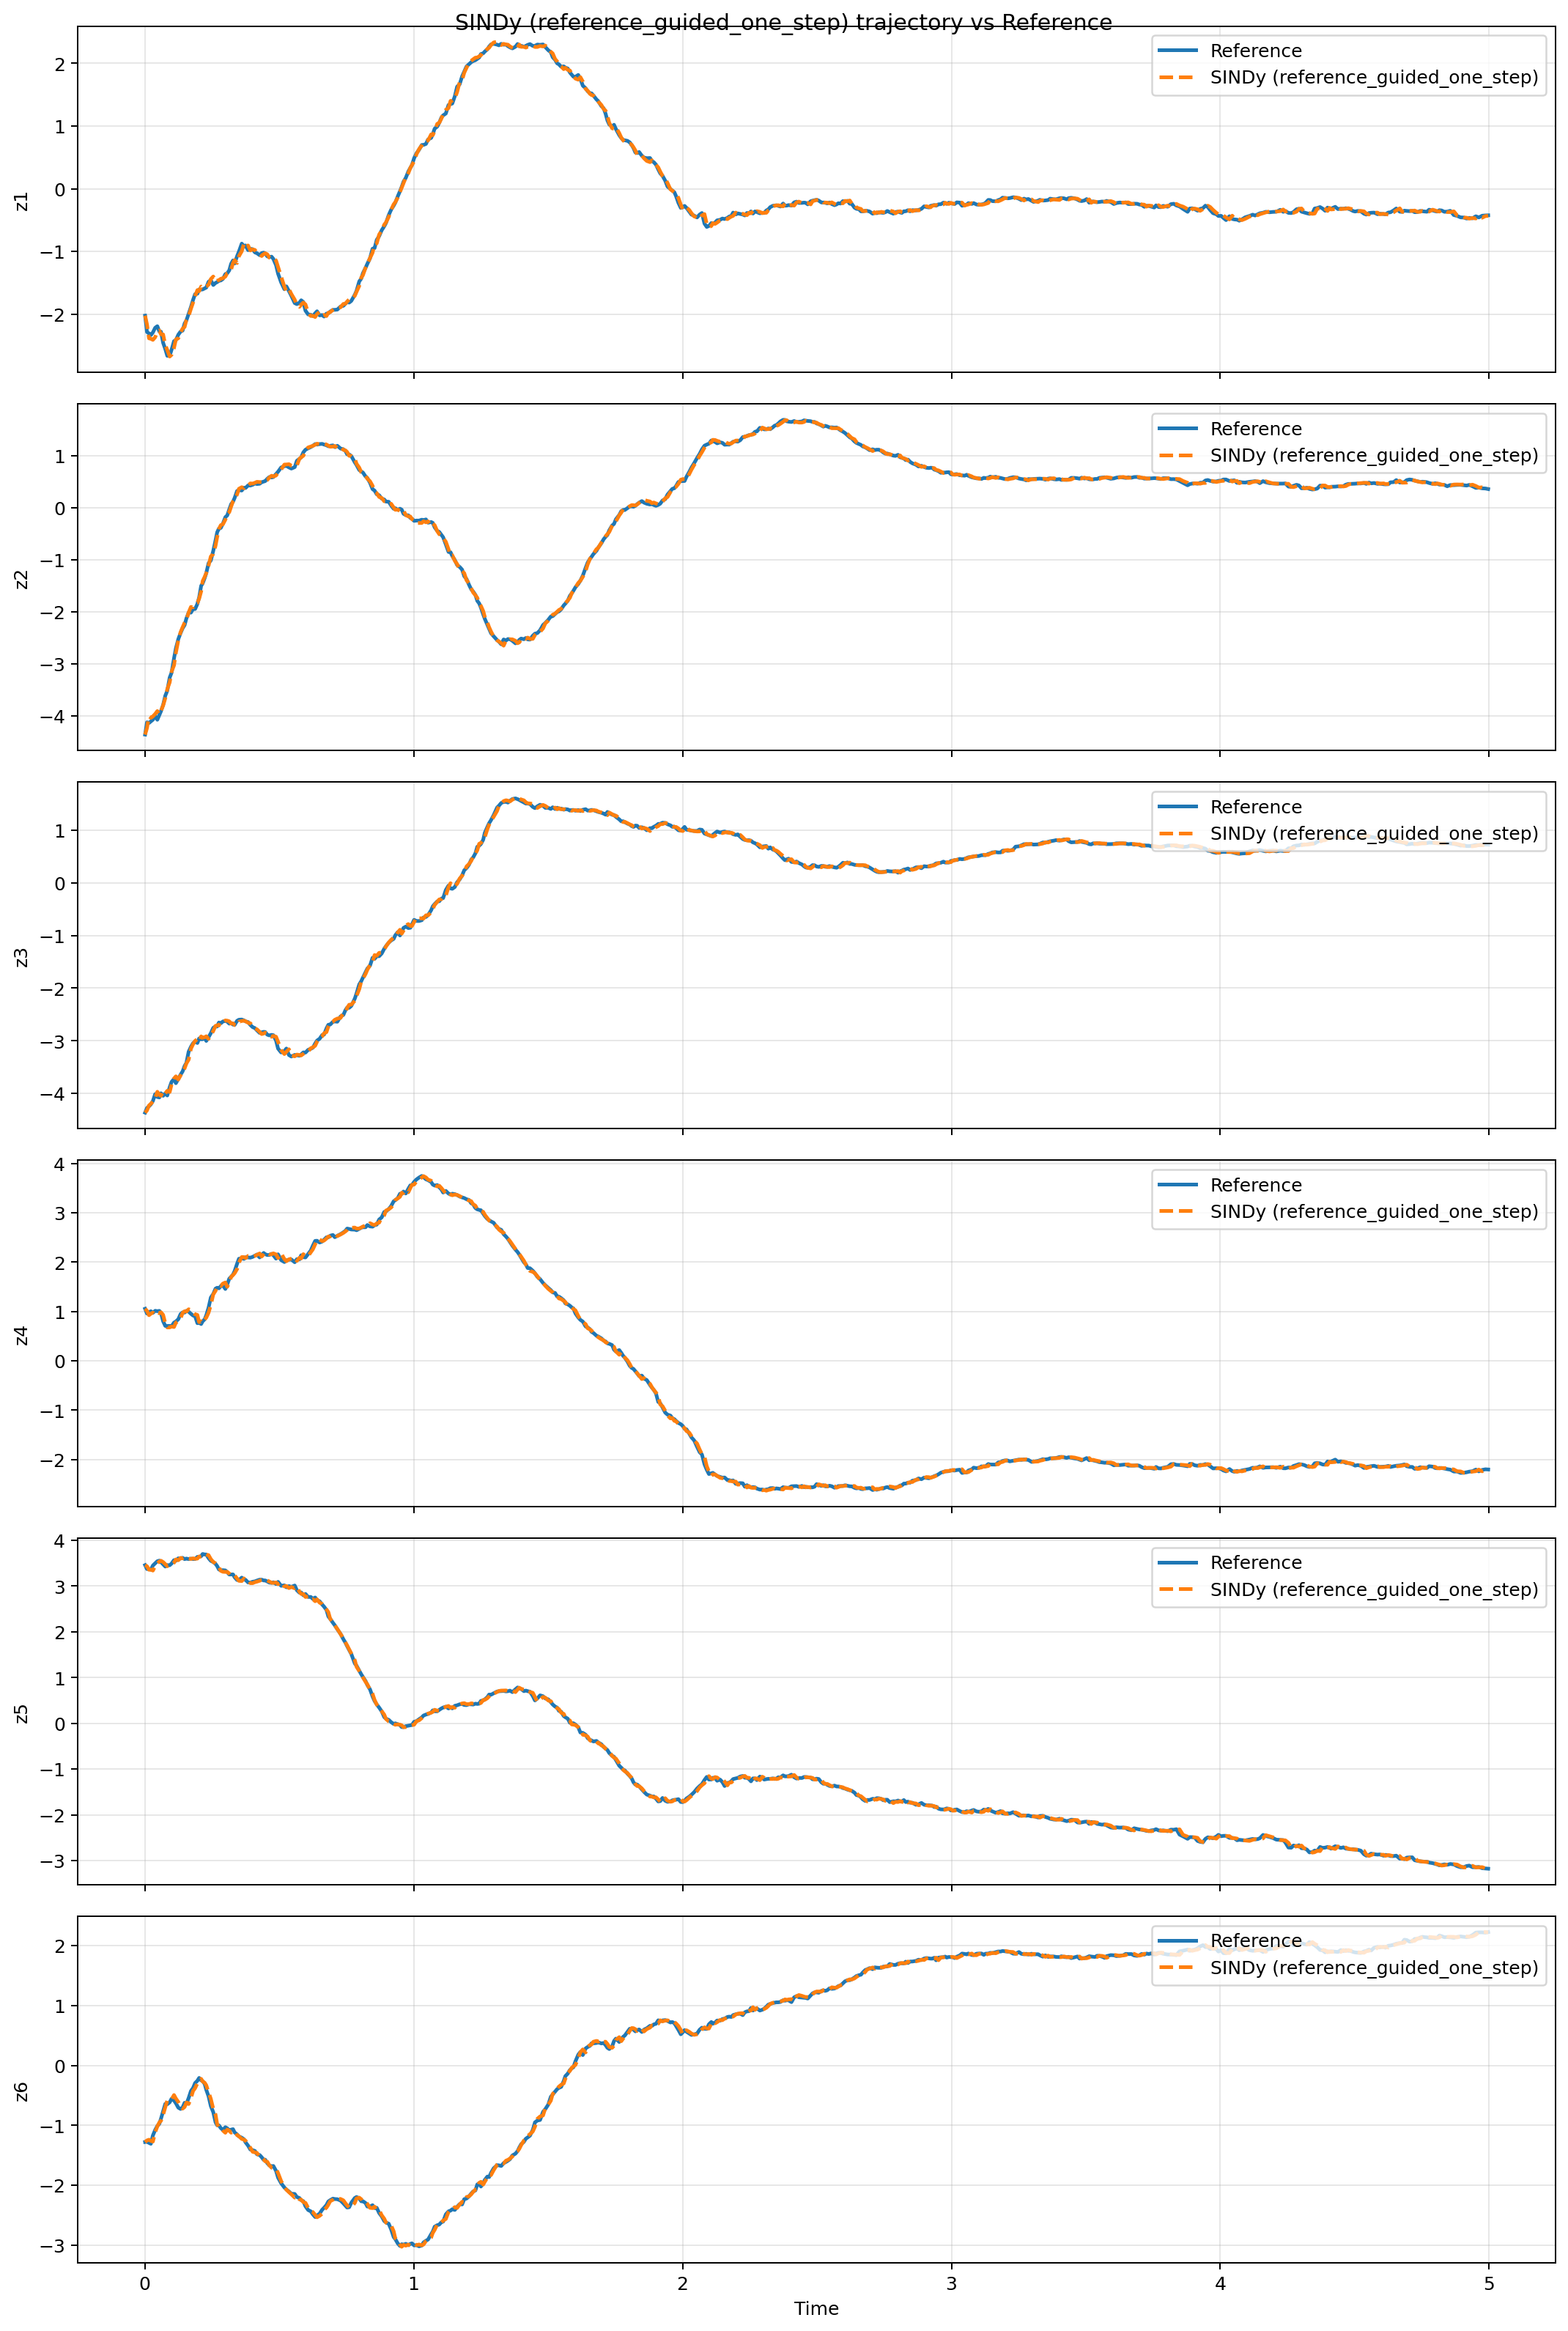
\includegraphics[width=\linewidth]{saes_traj.png}\caption{Fallback guiado.}\end{subfigure}
\caption{SAE--SINDy.}\end{figure}

\subsection{SAE--POD--SINDy}
A POD latente reduz oito coordenadas a quatro e conserva 96,6806\% da energia. Entre 48 candidatos, quatro foram aceitos. O selecionado usa ordem 1, Adalasso, $\alpha=0,1$, suavização 51, termos polinomiais e harmônicos no tempo e RK45. Possui 11 termos não nulos em 40, esparsidade 72,5\%.

\begin{table}[H]\centering\caption{Métricas SAE--POD--SINDy.}\label{tab:hyb}
\begin{tabular}{lr}\toprule Métrica&Valor\\\midrule
Energia POD latente&0,96681\\Erro de derivada / $R^2$&0,38822 / 0,84754\\Erro de um passo / $R^2$&0,03905 / 0,99847\\Integração livre&bem-sucedida\\Erro livre / $R^2$&0,64369 / 0,58567\\$R^2$ derivada: treino / validação&0,86213 / $-2,88257$\\\bottomrule\end{tabular}\end{table}
\lstinputlisting[style=sindyeq,caption={Equações completas SAE--POD--SINDy.}]{equacoes_sae_pod_sindy.txt}
\begin{figure}[H]\centering
\begin{subfigure}{.49\textwidth}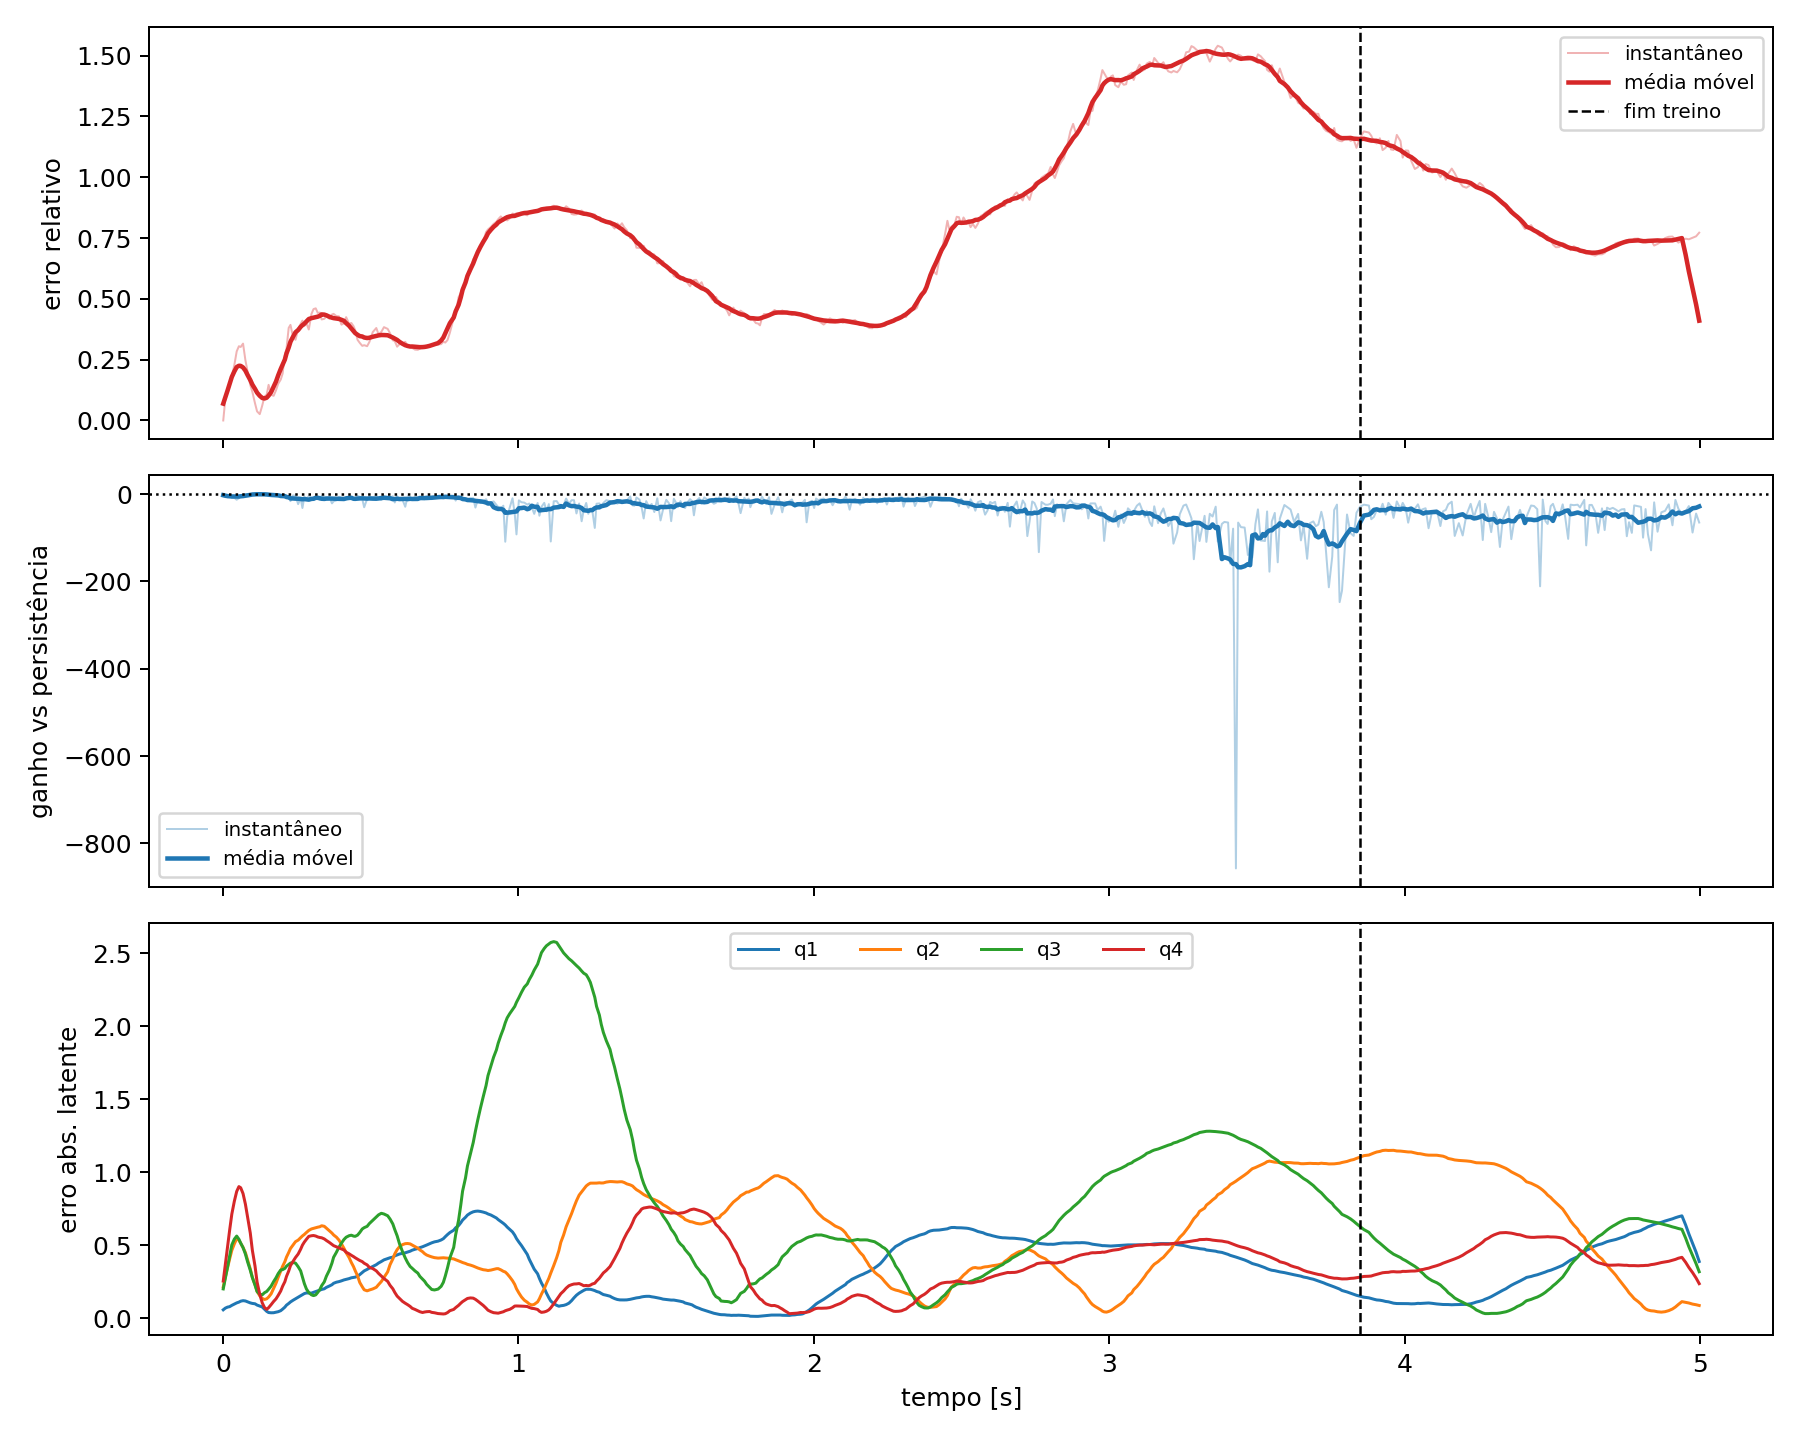
\includegraphics[width=\linewidth]{hyb_curves.png}\caption{Erros temporais.}\end{subfigure}
\begin{subfigure}{.49\textwidth}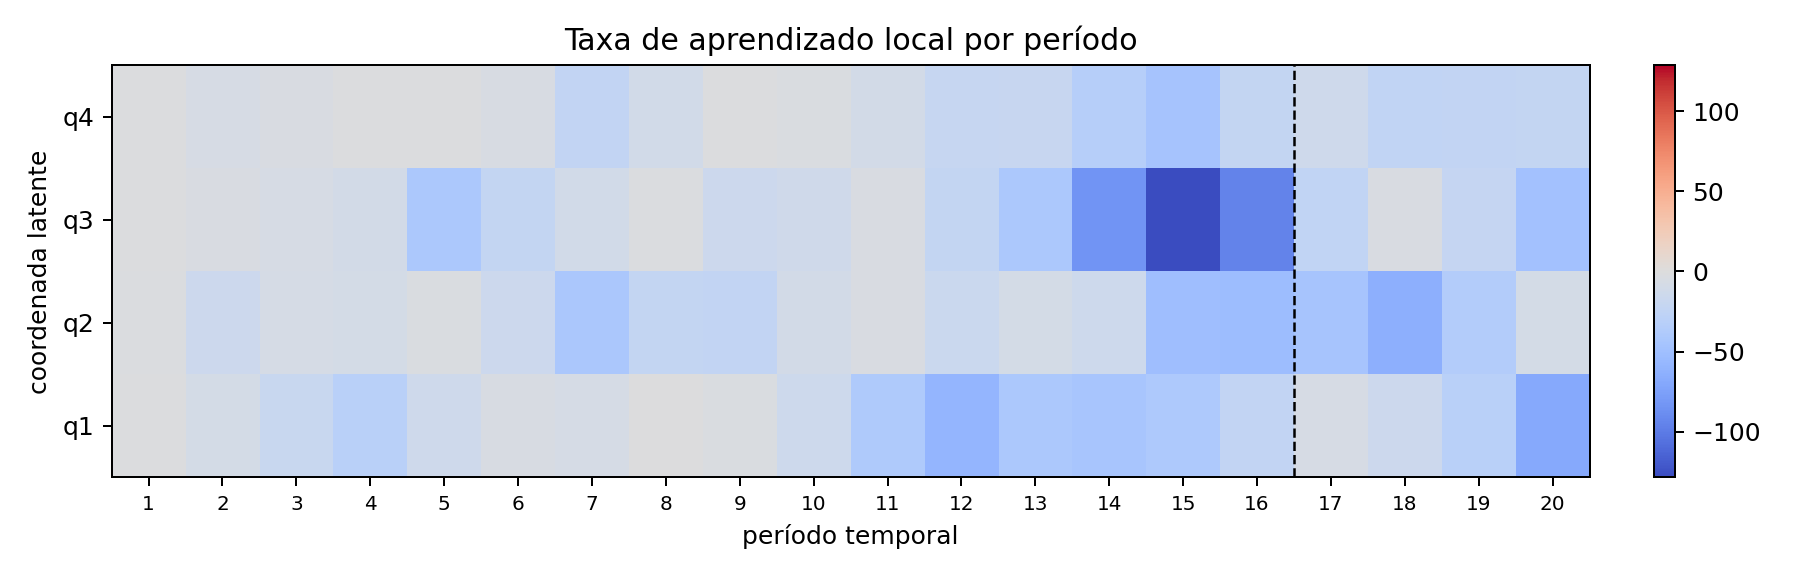
\includegraphics[width=\linewidth]{hyb_map.png}\caption{Coordenadas reduzidas.}\end{subfigure}
\caption{Diagnóstico do modelo estabilizado.}\end{figure}
\begin{figure}[H]\centering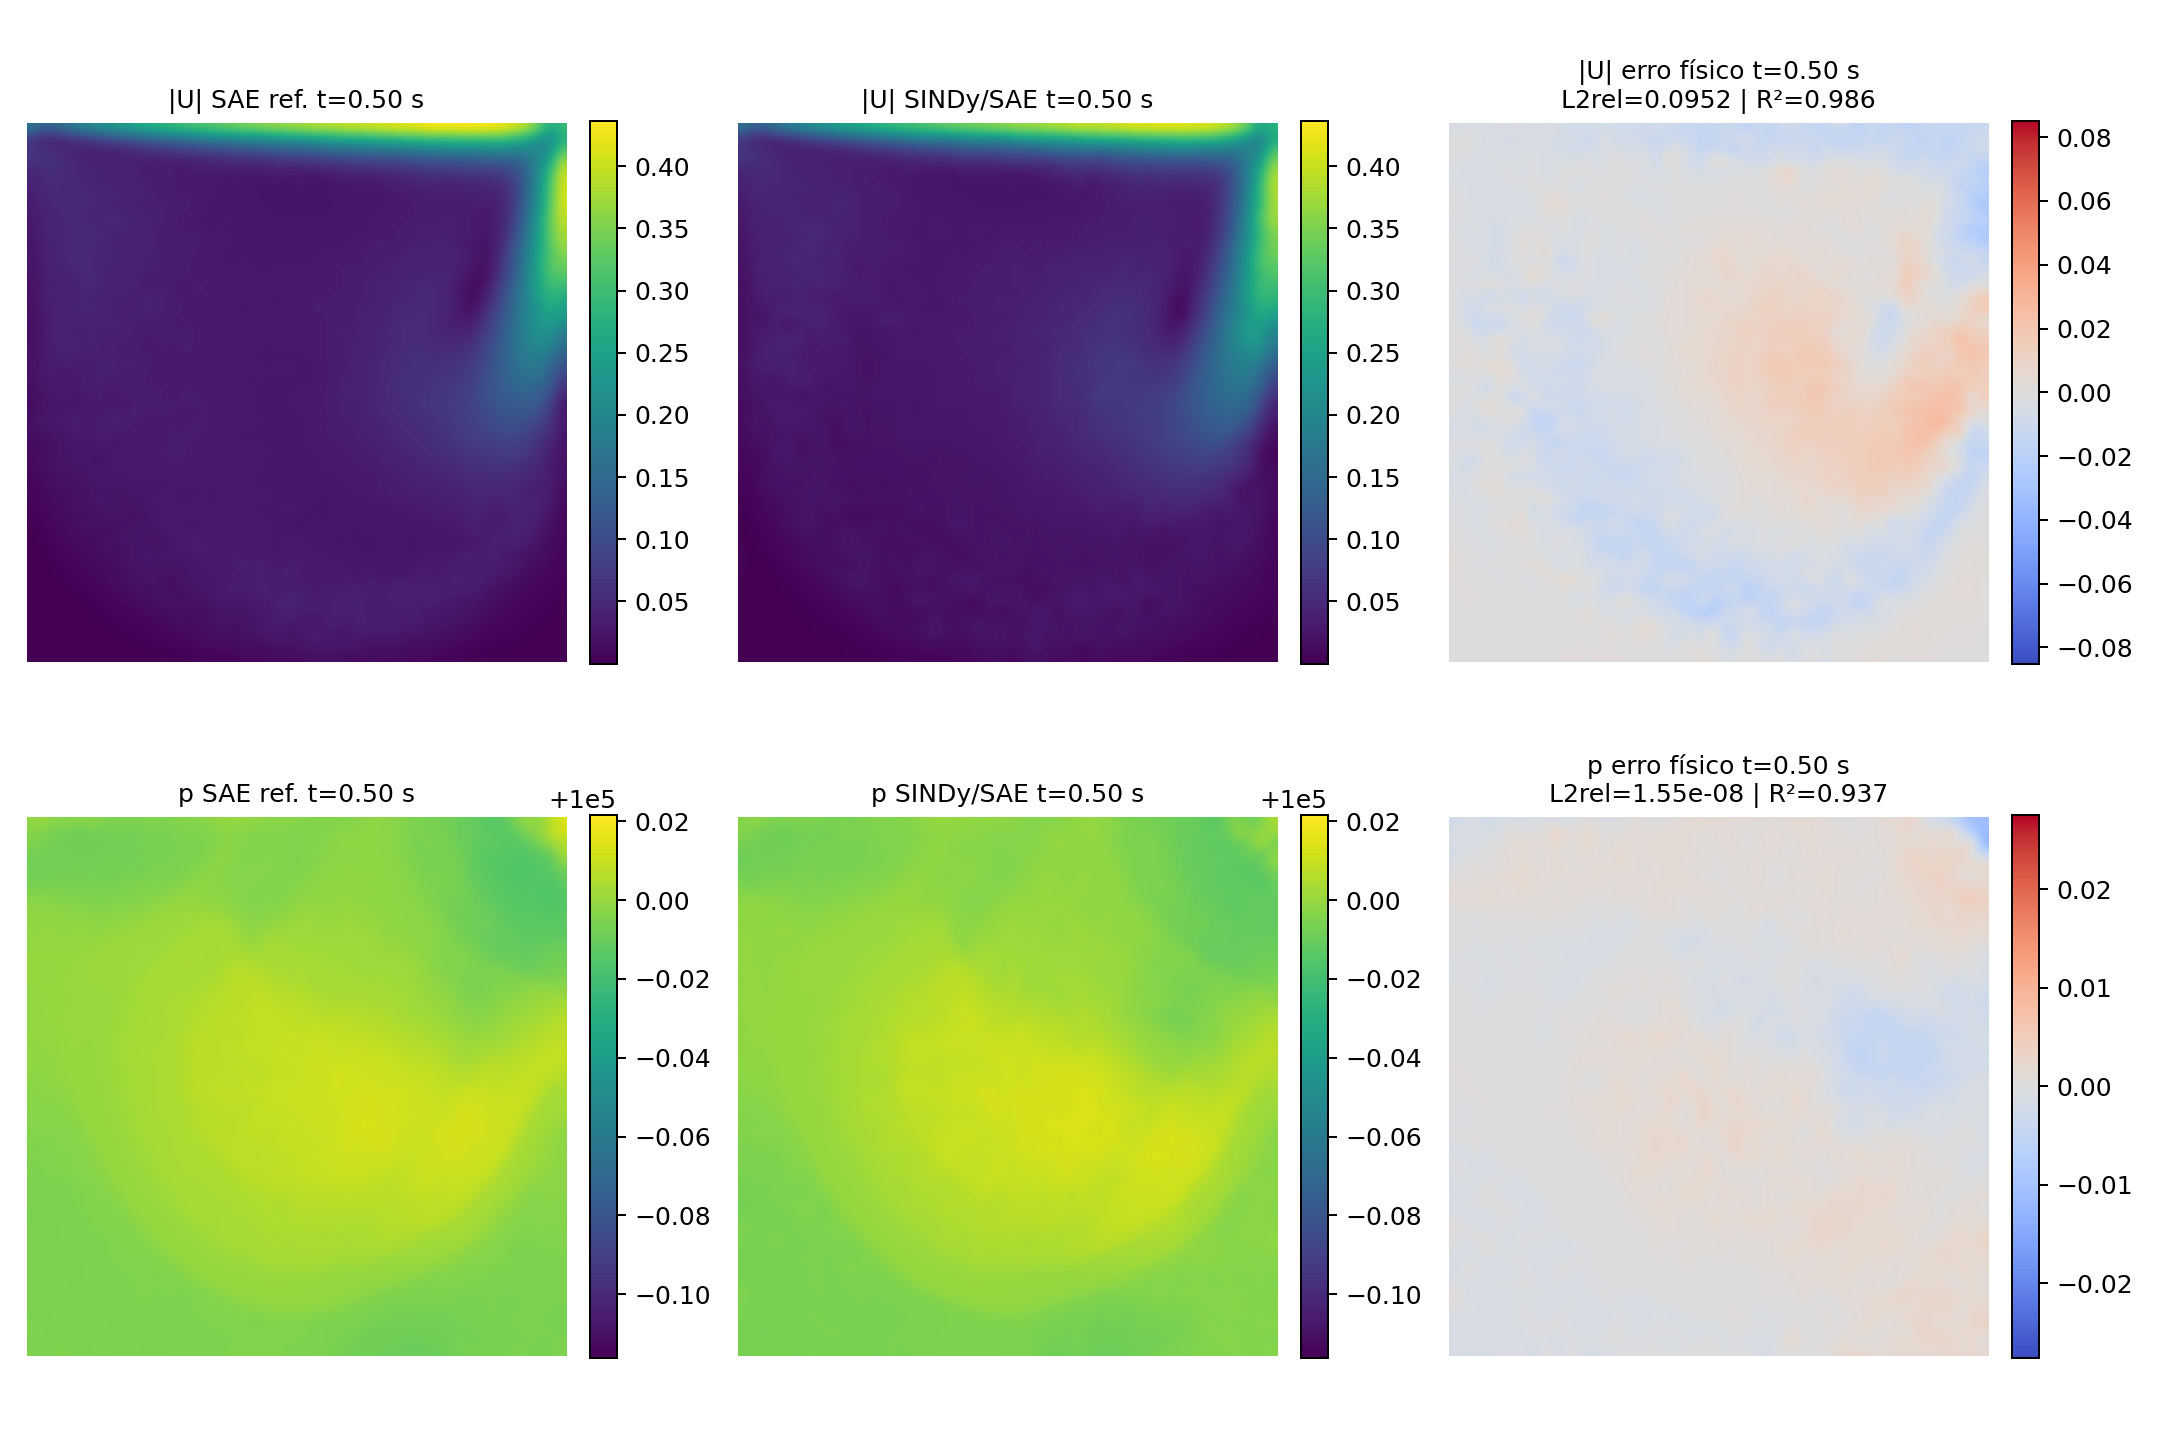
\includegraphics[width=.91\textwidth]{hyb_t05.png}\caption{Campos decodificados em $t\approx0,50\,\si{s}$.}\end{figure}
\begin{figure}[H]\centering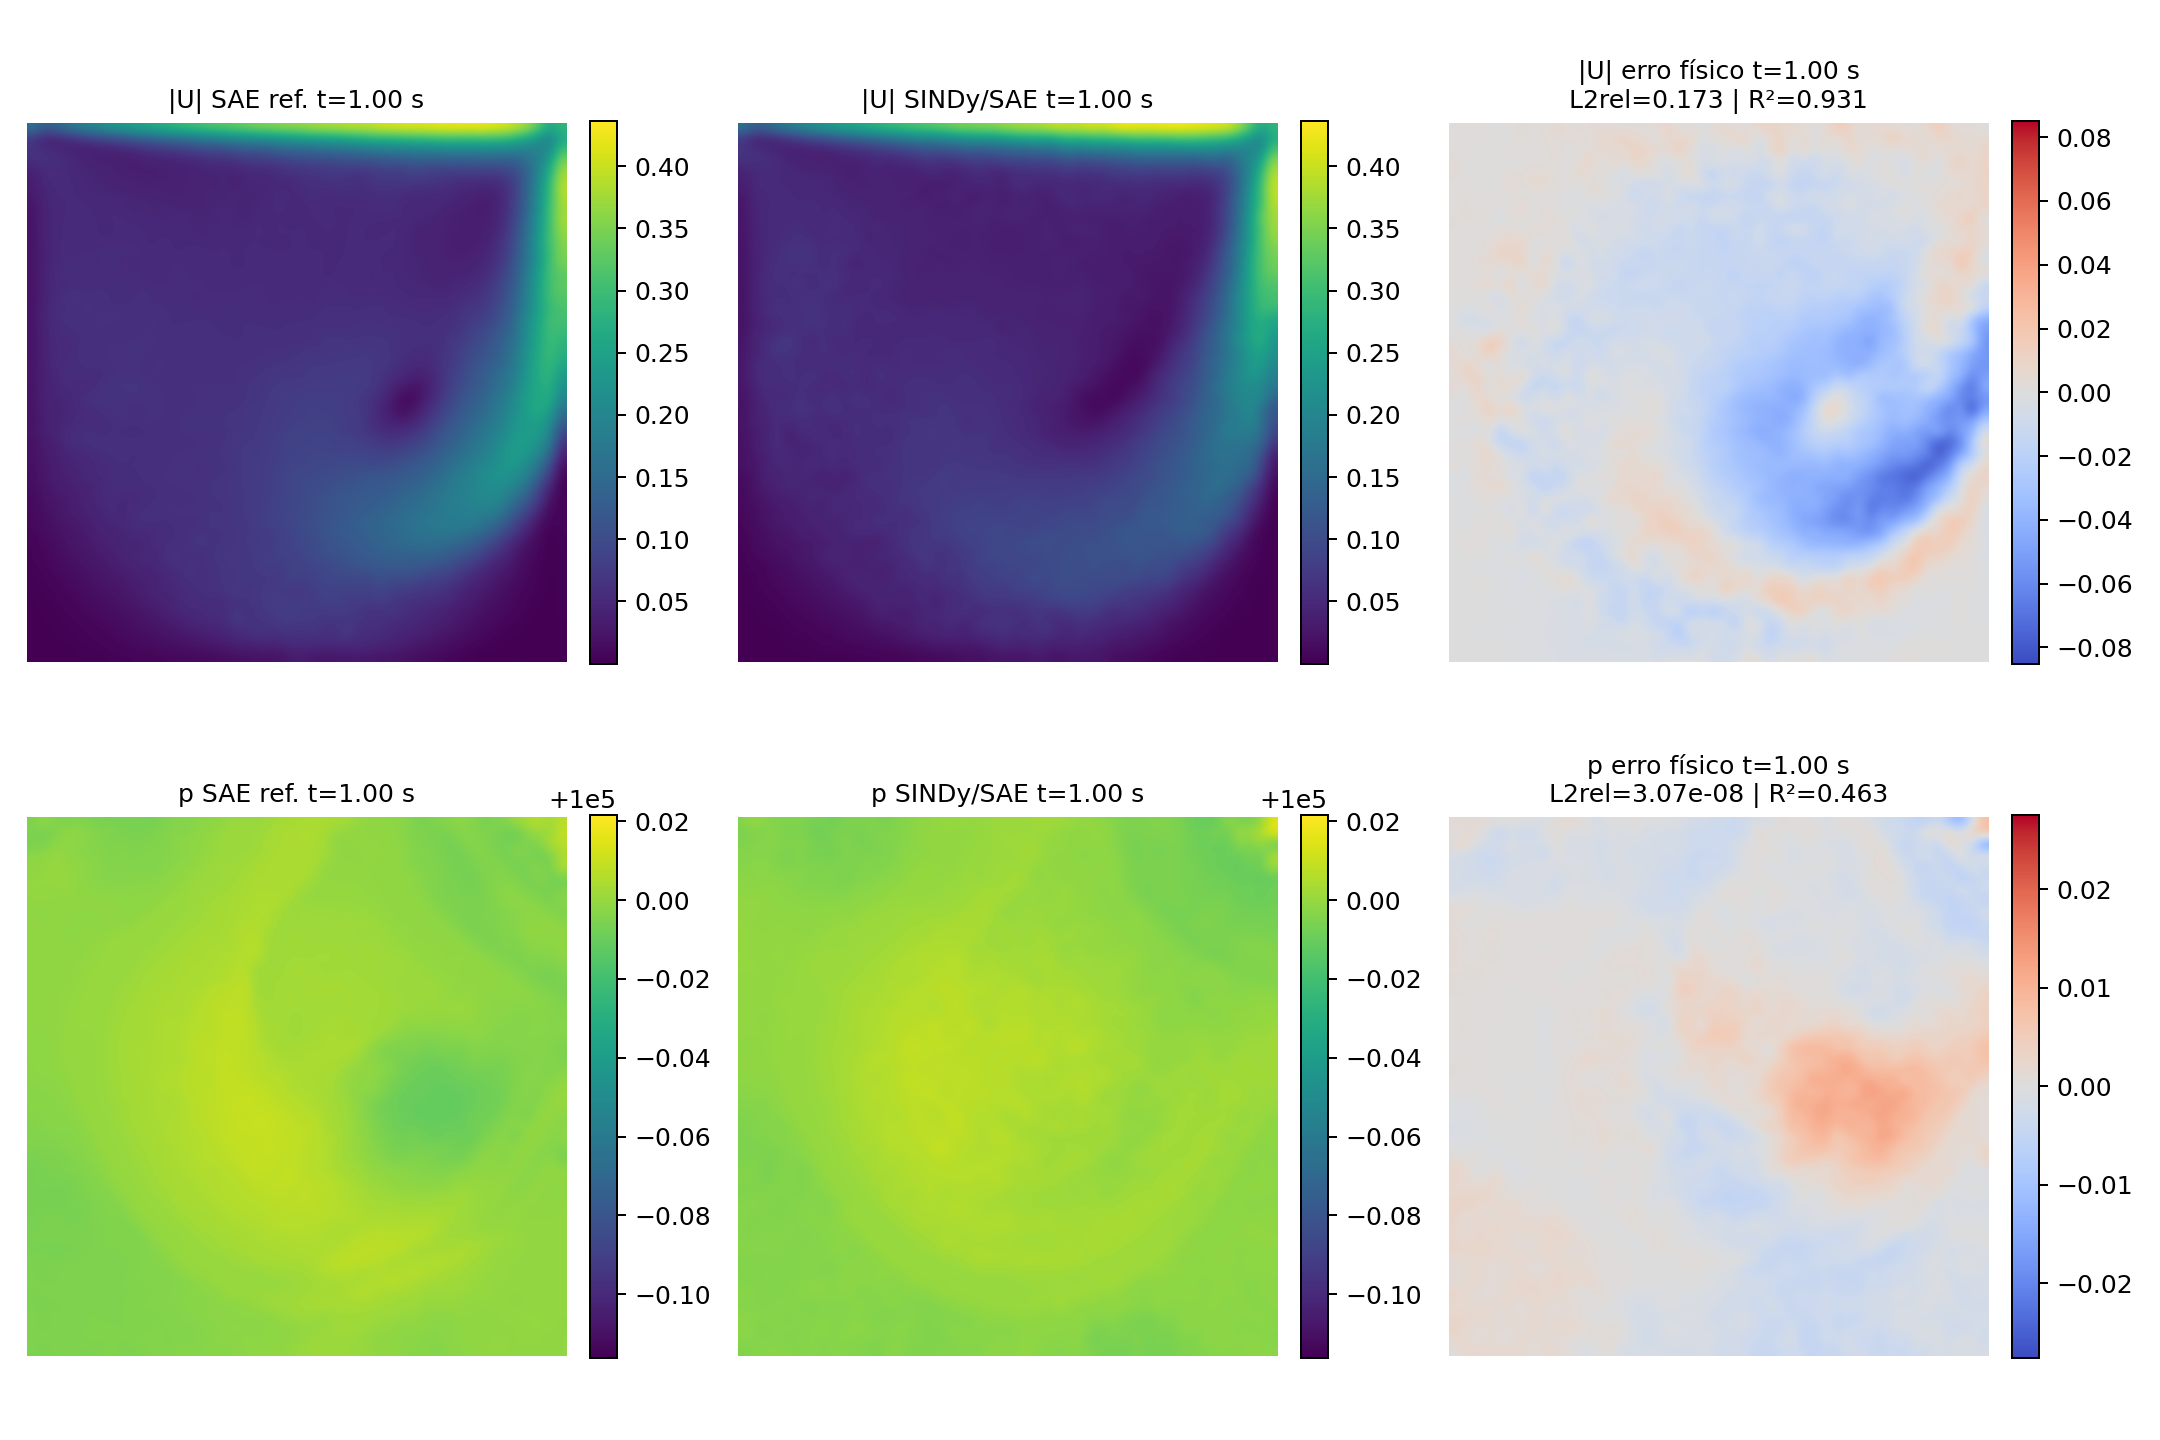
\includegraphics[width=.91\textwidth]{hyb_t10.png}\caption{Campos decodificados em $t\approx1,00\,\si{s}$.}\end{figure}

Para $t\approx0;0,25;0,50;0,75;1\,\si{s}$, os erros relativos de $|U|$ são 0,160; 0,212; 0,095; 0,116; 0,173 e os respectivos $R^2$ são 0,962; 0,938; 0,986; 0,974; 0,931. A pressão apresenta erro relativo muito pequeno devido ao grande nível médio ($\sim10^5\,\si{Pa}$); seu $R^2$ cai de 0,987 para 0,463, mostrando que erro relativo sem remoção da média é enganoso.

\subsection{Comparação OpenFOAM bruto--SINDy inválida}
No relatório salvo, para frações 0,25 a 1,00 o índice OpenFOAM fica congelado em 5645, com tempo assumido $1\,\si{s}$, enquanto o SINDy avança até 4,9965 s. O erro de $|U|$ chega a 5,103 e $R^2=-109,63$, mas esses valores misturam erro de modelo e desalinhamento temporal. A figura abaixo documenta a falha, não o desempenho físico.
\begin{figure}[H]\centering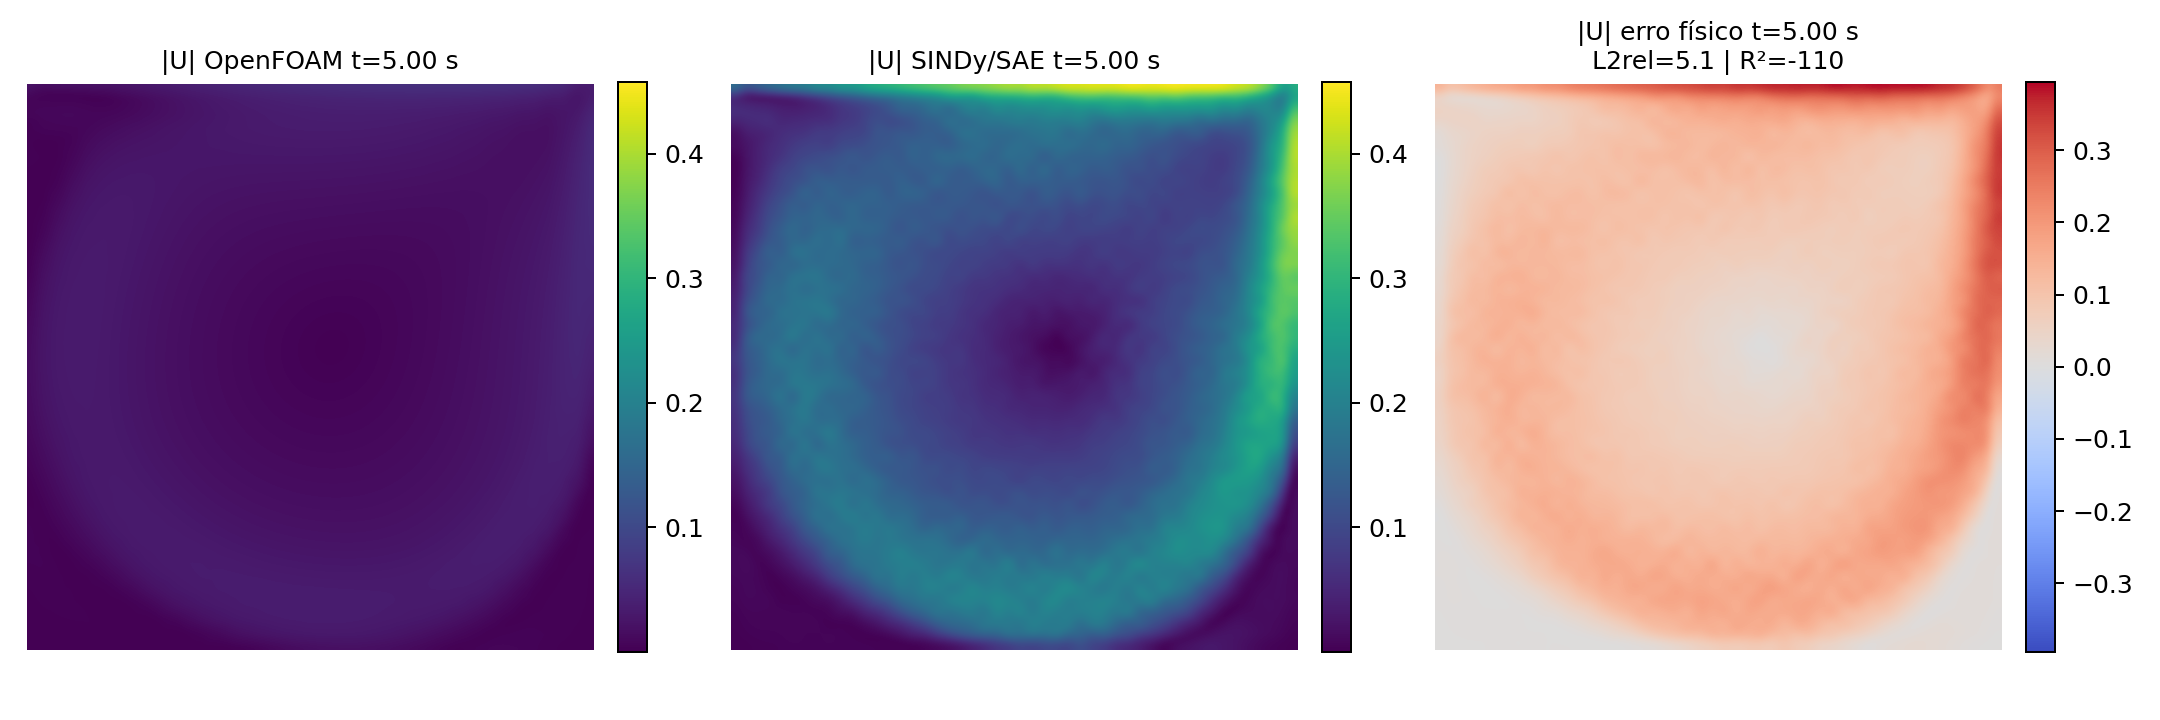
\includegraphics[width=.91\textwidth]{hyb_raw_bad.png}\caption{Comparação bruta no final: diferença temporal de 3,9965 s; resultado inválido para validação.}\end{figure}

\subsection{Validação direta corrigida}
Foi implementada uma validação independente que lê $U,p,T,k$ diretamente dos diretórios OpenFOAM, usa os tempos físicos reais e interpola para a mesma grade $48\times48$ do SAE. Ela não depende da POD incorreta. O desalinhamento temporal máximo nos cinco instantes ficou abaixo de $1,1\times10^{-7}\,\si{s}$.

\begin{table}[H]\centering\caption{Validação direta da trajetória livre contra OpenFOAM.}\label{tab:direct}
\begin{tabular}{rcccc}\toprule
$t$ [s]&erro $|U|$&$R^2(|U|)$&erro $k$&$R^2(k)$\\\midrule
1,2500&0,1281&0,9579&0,0242&0,9993\\
2,4985&0,1757&0,8815&0,0683&0,9950\\
3,7430&0,1556&0,9054&0,1434&0,9781\\
4,9965&0,2447&0,7569&0,3142&0,8955\\\bottomrule
\end{tabular}\end{table}

Em $t=0,001\,\si{s}$, o erro relativo da velocidade é artificialmente enorme porque a referência ainda é quase nula; essa métrica não é informativa nesse instante. Para pressão e temperatura, o erro relativo bruto é da ordem de $10^{-7}$--$10^{-8}$ devido ao grande valor médio. Após remover a média, os erros são altos e o $R^2$ de $T$ permanece próximo de zero ou negativo; portanto, médias termodinâmicas corretas não significam que as flutuações foram capturadas.

\begin{figure}[H]\centering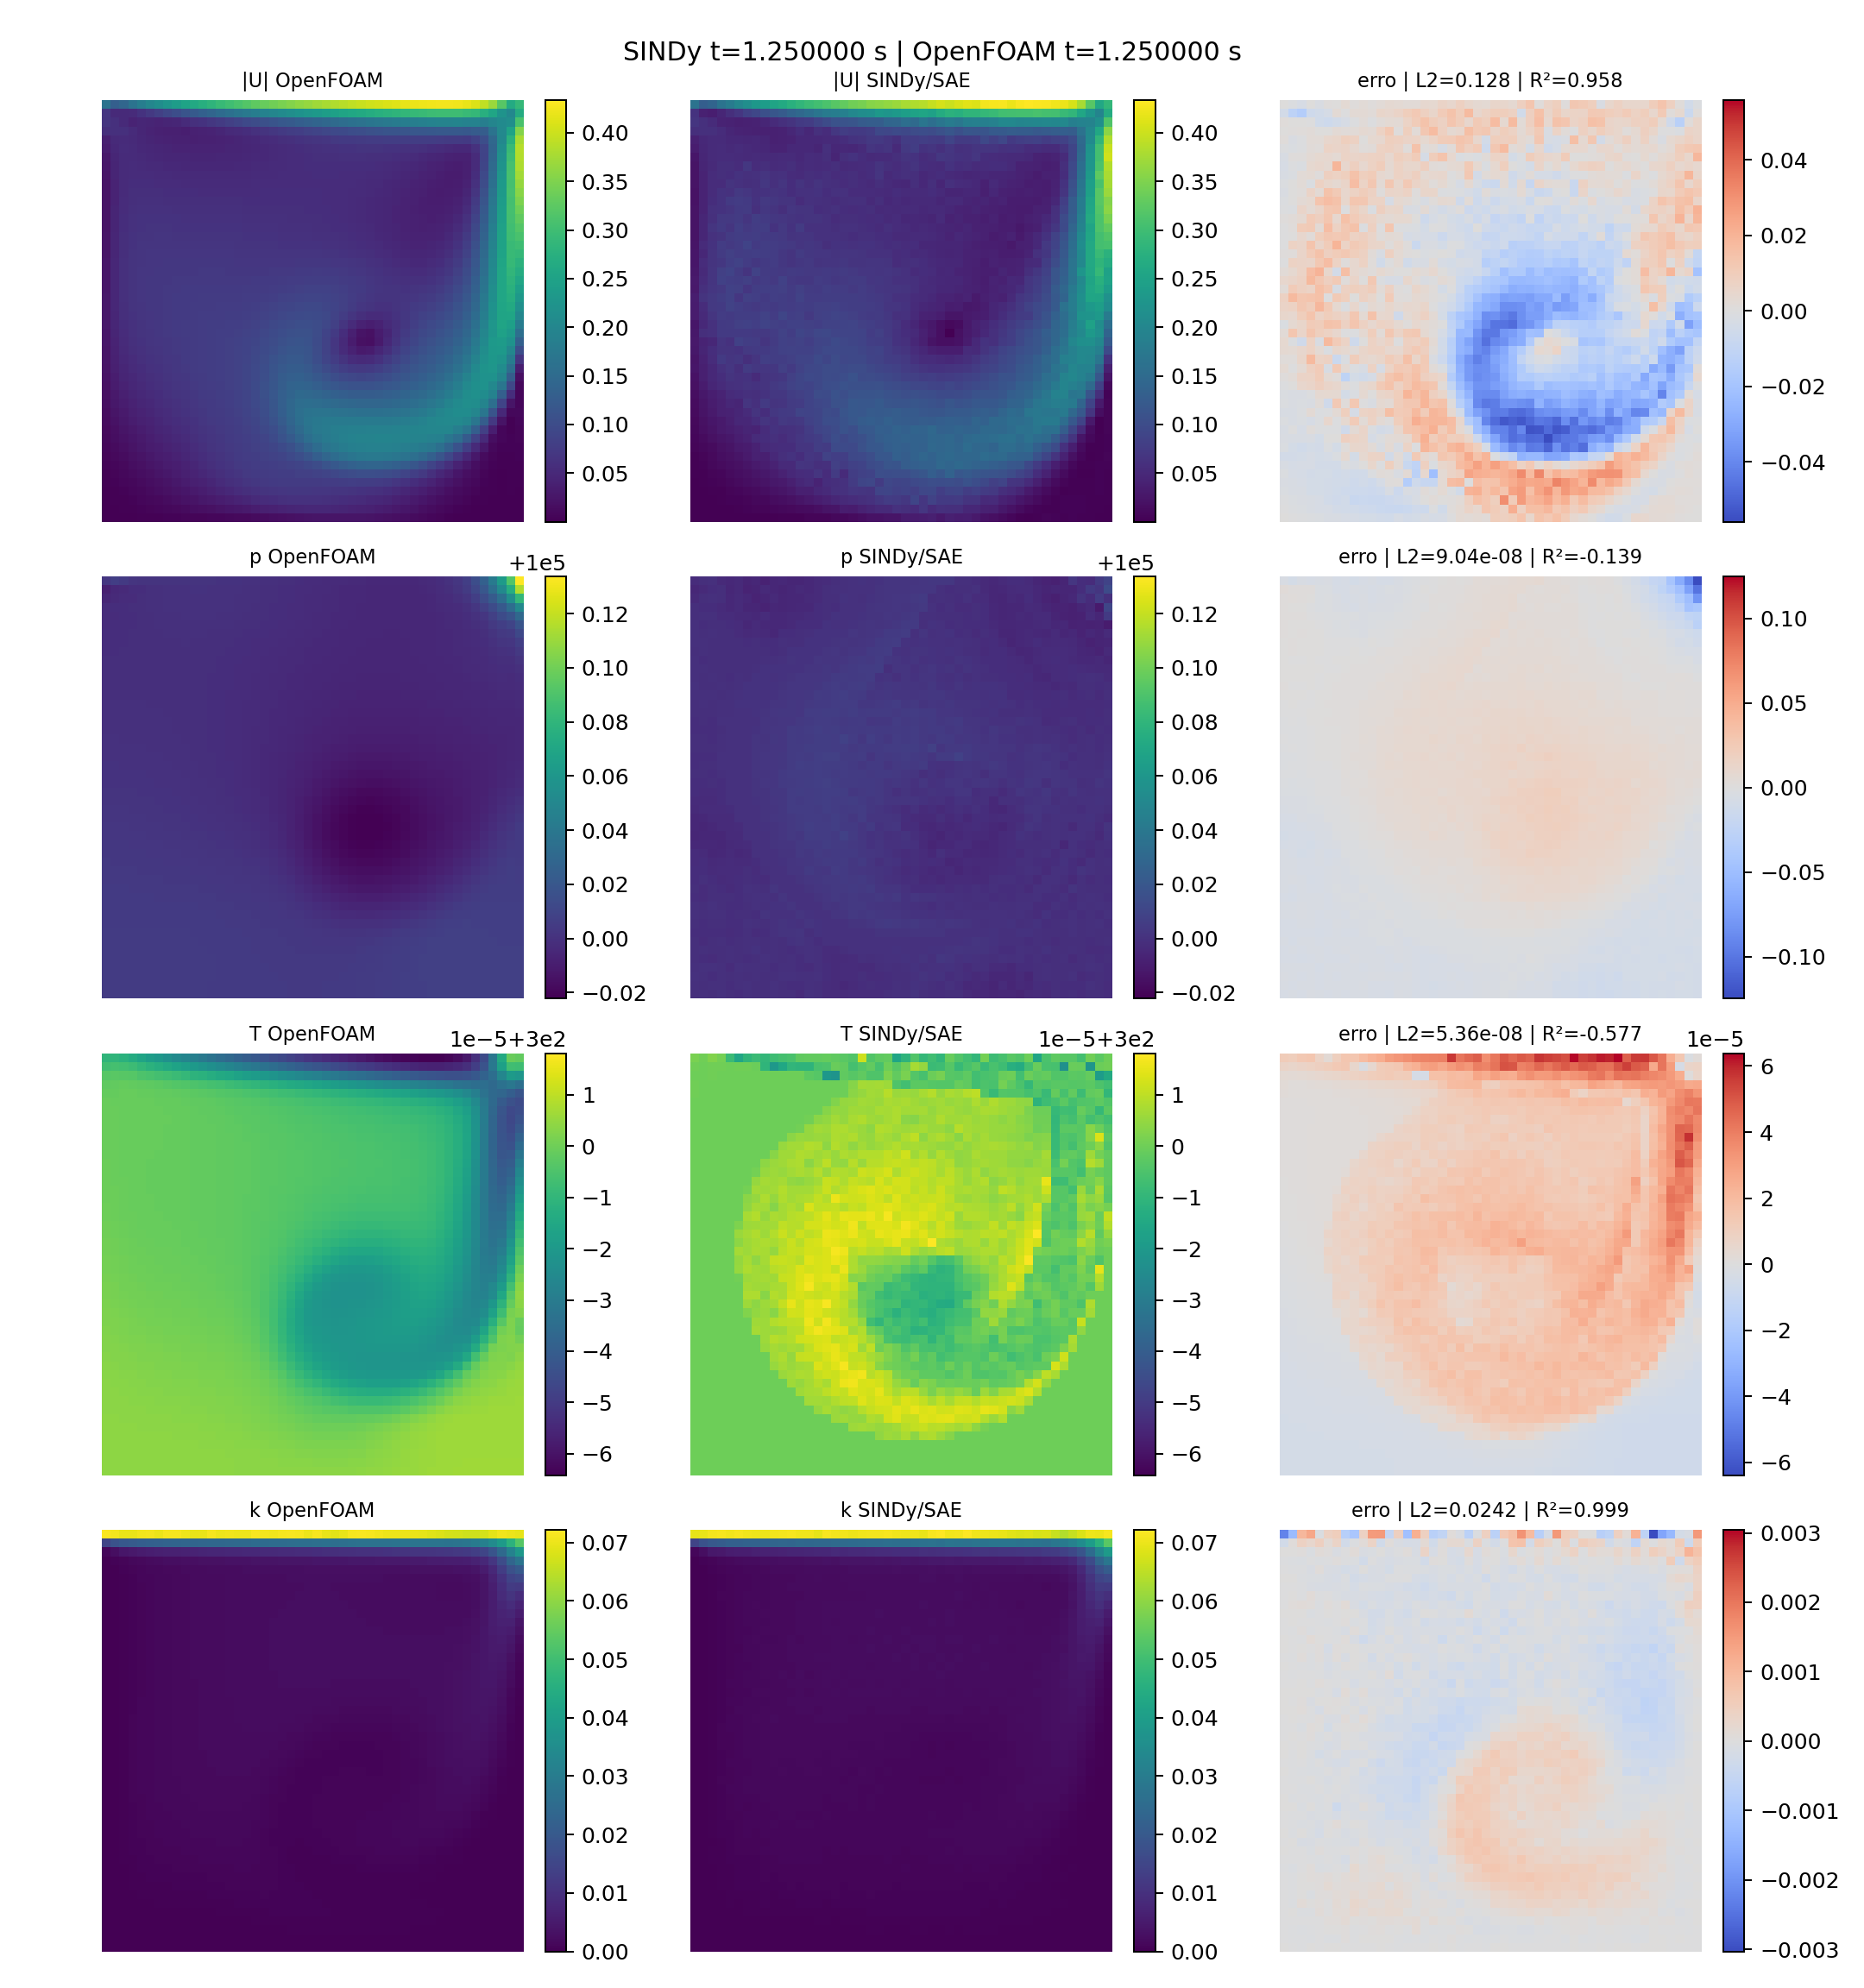
\includegraphics[width=.91\textwidth]{direct_t125.png}\caption{Validação direta corrigida em $t=1,25\,\si{s}$.}\end{figure}
\begin{figure}[H]\centering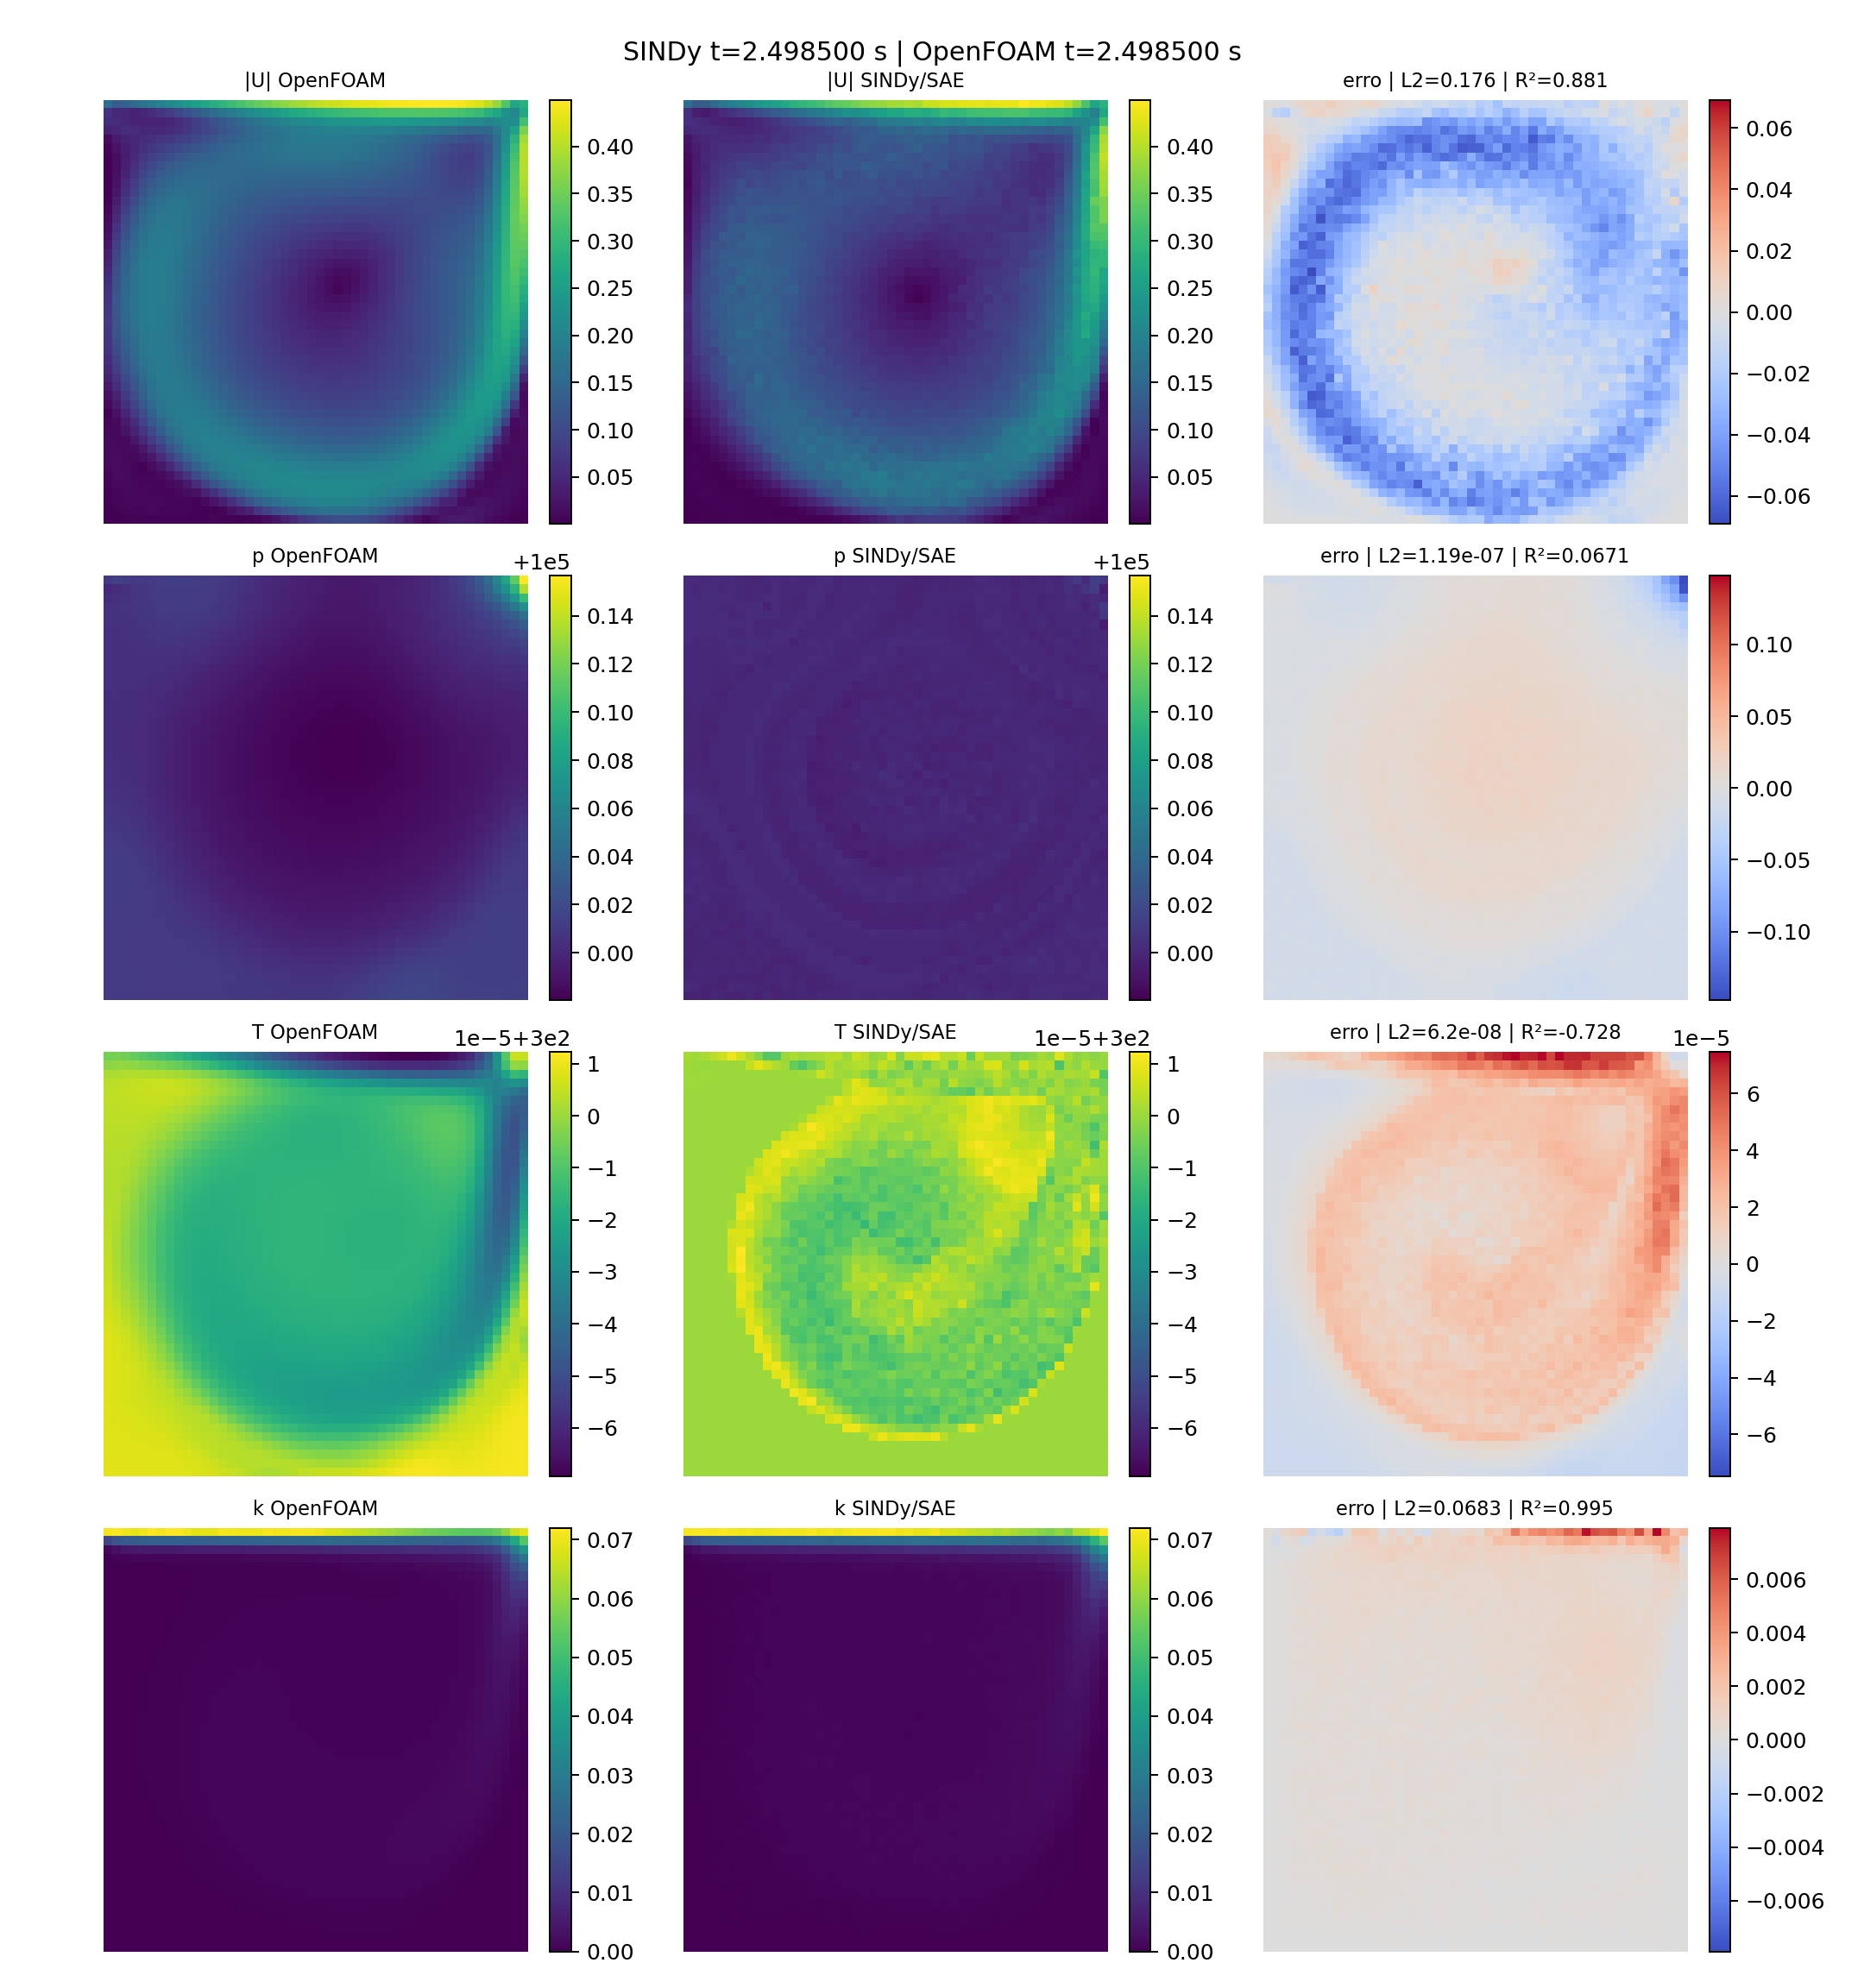
\includegraphics[width=.91\textwidth]{direct_t250.png}\caption{Validação direta corrigida em $t\approx2,50\,\si{s}$.}\end{figure}
\begin{figure}[H]\centering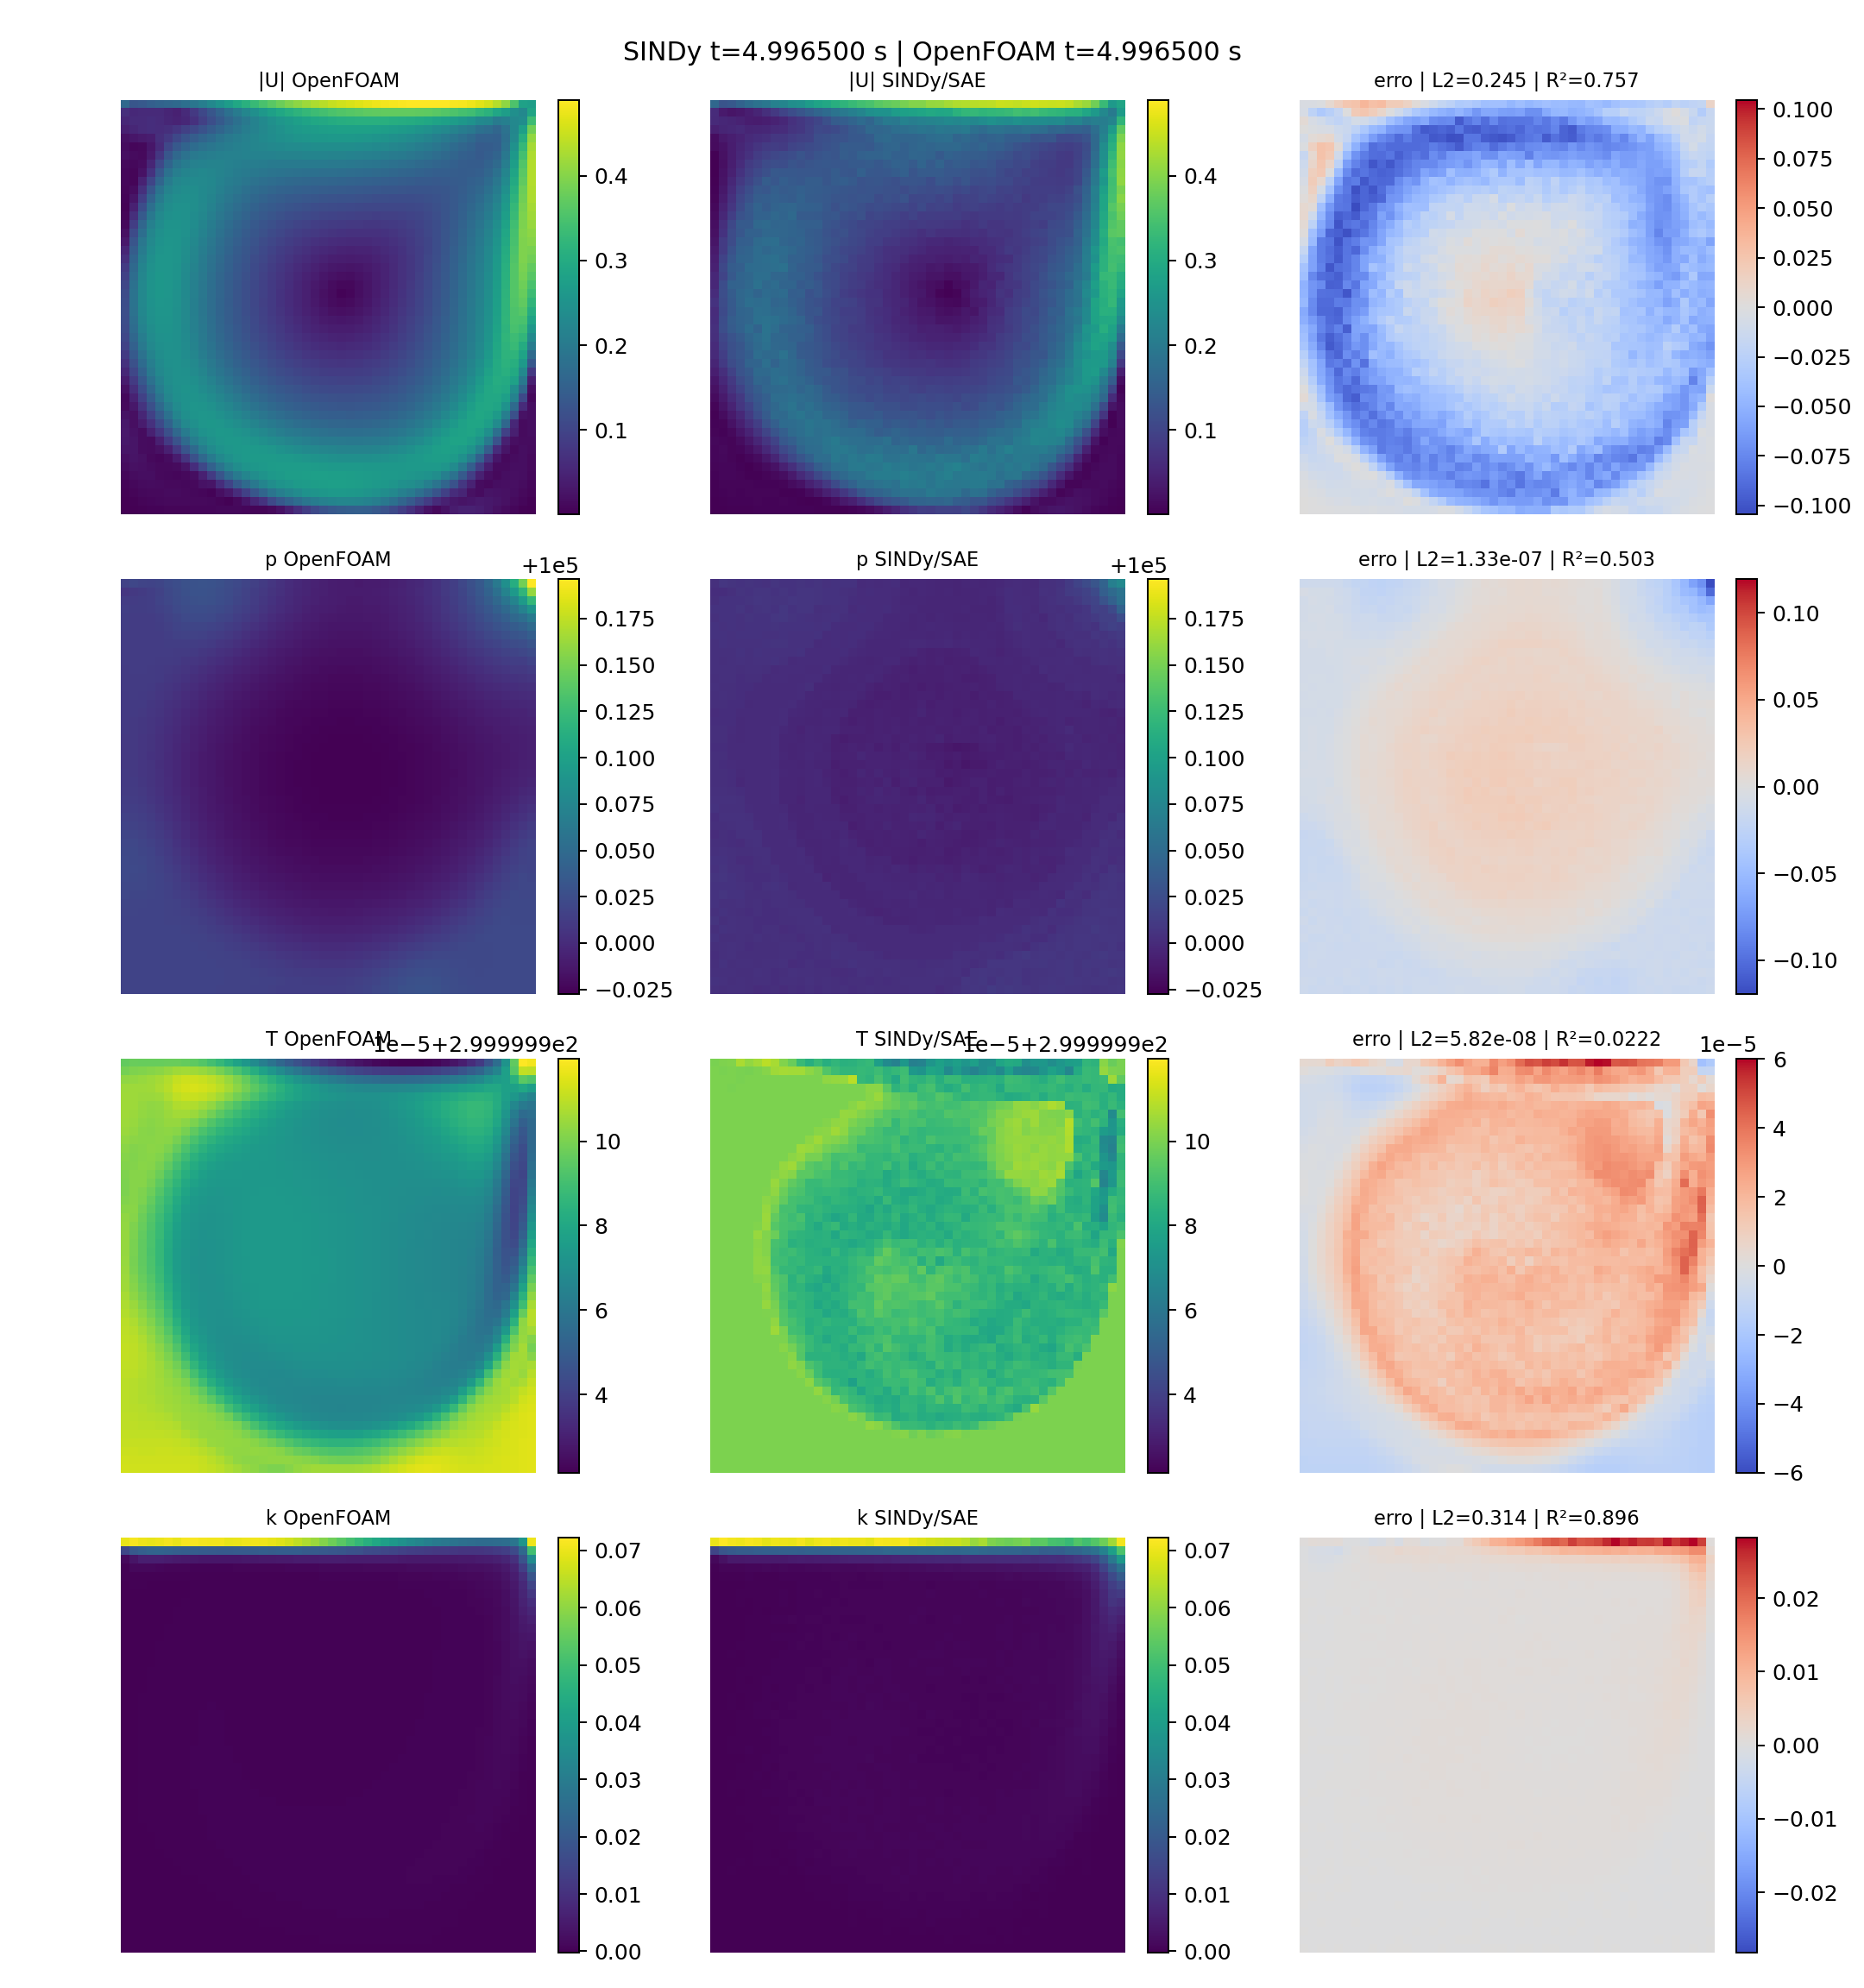
\includegraphics[width=.91\textwidth]{direct_t500.png}\caption{Validação direta corrigida em $t=4,9965\,\si{s}$.}\end{figure}

\section{Papel estabilizador da POD e comparação com a literatura}
Lin, Xiao e Fang~\cite{lin2024} propõem SAE--POD--SINDy para reduzir a aleatoriedade e melhorar o condicionamento do espaço latente antes da regressão esparsa. A POD centraliza, gira e ordena os códigos do SAE. Neste caso, SAE--SINDy falha, enquanto SAE--POD--SINDy integra até o final, apoiando qualitativamente esse papel.

Entretanto, o artigo enfatiza que uma transformação POD equidimensional pode organizar os latentes sem necessariamente truncá-los. Aqui há redução 8 para 4, com perda de 3,32\% da energia. Além disso, o $R^2$ de derivada na validação é $-2,88$ e o erro livre é 0,644. Portanto, a integração foi estabilizada, mas a lei dinâmica ainda generaliza mal.

\begin{table}[H]\centering\caption{Representação e dinâmica.}\label{tab:comp}
\begin{tabularx}{\textwidth}{>{\bfseries}l X X}\toprule Método&Representação&Captura dinâmica observada\\\midrule
POD&corrigida: 99,988\% em 50 modos&não se aplica isoladamente\\
SAE&$R^2\approx0,81$--0,83&não se aplica isoladamente\\
POD--SINDy&reexecutado com campos corretos&erro local melhora; integração livre ainda falha\\
SAE--SINDy&latentes dos campos corretos&livre falha; apenas um passo é bom\\
SAE--POD--SINDy&96,68\% da energia latente&livre funciona; erro 0,644 e $R^2=0,586$\\\bottomrule\end{tabularx}\end{table}

\section{Pontos positivos, limitações e recomendações}
\subsection*{Pontos positivos}
\begin{itemize}
\item malha ortogonal e condições de contorno claras;
\item SAE emprega campos relevantes para cavidade compressível e tem validação temporal consistente na reconstrução;
\item equações e métricas completas estão salvas;
\item a POD latente torna a integração livre possível, com modelo relativamente esparso;
\item reconstrução de velocidade nos primeiros 1 s apresenta $R^2>0,93$ nos tempos amostrados.
\end{itemize}
\subsection*{Limitações}
\begin{itemize}
\item os artefatos POD legados permanecem inválidos; a versão corrigida foi salva separadamente para rastreabilidade;
\item sequência OpenFOAM contém apenas 5646 dos 10001 passos nominais;
\item POD--SINDy e SAE--SINDy falham em integração livre;
\item forte sobreajuste de derivadas no modelo híbrido;
\item comparador bruto antigo limita incorretamente a referência a 1 s; foi substituído por validação direta, mas mantido apenas para rastreabilidade;
\item termos explícitos em tempo reduzem autonomia e transferibilidade;
\item ausência de validação clássica da cavidade e de independência de malha/passo.
\end{itemize}
\subsection*{Recomendações}
\begin{enumerate}
\item Usar exclusivamente a POD corrigida com $U,p,T,k$; não promover automaticamente os arquivos legados.
\item Manter a nova falha explícita quando um campo obrigatório não existir, em vez de zeros silenciosos.
\item Usar a nova validação direta com alinhamento pelos tempos físicos reais.
\item Comparar POD latente 8--8 e 8--4 para separar rotação estabilizadora de truncamento.
\item Selecionar o SINDy pelo erro de integração livre em validação e pelo $R^2$ de derivada fora do treino.
\item Validar perfis de velocidade nas linhas centrais, posição/intensidade dos vórtices e Reynolds efetivo.
\end{enumerate}

\section{Conclusão}
O SAE é a representação mais coerente fisicamente porque usa $U,p,T,k$. A POD salva apresenta números de reconstrução excelentes, mas seus canais foram configurados para outro problema. Os modelos SINDy puros não sustentam integração livre. A POD aplicada aos latentes estabiliza a integração, em concordância qualitativa com Lin, Xiao e Fang, mas o erro livre de 0,644 e a forte degradação das derivadas em validação impedem afirmar captura precisa. A validação direta corrigida mostra desempenho razoável para $|U|$ e $k$ ao longo de 5 s, com deterioração no final, enquanto as flutuações de $p$ e $T$ são mal descritas. Os códigos de POD e validação temporal foram corrigidos e o POD--SINDy foi reexecutado com os campos corretos. A falha persistente da integração livre confirma que o problema dinâmico não era causado apenas pelos campos copiados.

\appendix\section{Arquivos auditados}
\small\begin{itemize}
\item OpenFOAM: \path{system/controlDict}, \path{blockMeshDict}, \path{fvSchemes}, \path{fvSolution}, \path{constant/physicalProperties}, \path{momentumTransport}.
\item POD: \path{POD/resultados/resultados_pod_completos.npz}.
\item SAE: \path{SAE/resultados/sae_dense.keras}, \path{sae_dense_metrics.npz}, \path{latents.npz}.
\item SINDy: arquivos JSON, NPZ, CSV e TXT em \path{SINDy/resultados}.
\end{itemize}\normalsize
\begin{thebibliography}{9}
\bibitem{sirovich} L. Sirovich. Turbulence and the dynamics of coherent structures. \emph{Quarterly of Applied Mathematics}, 45, 1987.
\bibitem{hinton} G. E. Hinton e R. R. Salakhutdinov. Reducing the dimensionality of data with neural networks. \emph{Science}, 313, 2006.
\bibitem{brunton} S. L. Brunton, J. L. Proctor e J. N. Kutz. Discovering governing equations from data by sparse identification of nonlinear dynamical systems. \emph{PNAS}, 113, 2016.
\bibitem{lin2024} X. Lin, D. Xiao e F. Fang. Data discovery of low dimensional fluid dynamics of turbulent flows. \emph{arXiv:2401.05449}, 2024. \href{https://arxiv.org/abs/2401.05449}{arxiv.org/abs/2401.05449}.
\bibitem{openfoam} OpenFOAM Foundation. \emph{OpenFOAM 13 documentation}.
\end{thebibliography}
\end{document}
